\chapter{Experimentations}
\chaptermark{Experimentations}
\label{chap:experimentations}
\graphicspath{{./chapters/6-experiments/figs/}}


% \modif{TODO add total number of annotated elements for each category and report the diversity of style, format, publishing from the IJDAR paper}

% Abstract-----------------------------------------------------
With the analysis and processing of data comes the need of the output results evaluation.
Traditionally, this evaluation is made by validating the results of an algorithm with a ground truth that represents what an ideal output should be\cite{pascal-voc-2012, smeaton2006evaluation, griffinHolubPerona}.
Ideally, such a ground truth is made publicly available so anyone can challenge his own algorithm to the community \cite{lamiroy:inria-00537035}.
This can be applied to any kind of results from image segmentation to classification or information retrieval.
In this chapter we present the dataset and ground truth we provided to evaluate comic book related works.
We describe the metrics we used to evaluate each of the contributions proposed in \ch{chap:sequential}, \ch{chap:independent} and \ch{chap:knowledge} and evaluate our work compared to previous works from the literature.
\modif{Note that we call these three approaches Method I (independent), Method S (sequential) and Method K (knowledge-driven) respectively in the rest of this chapter.}

%The evaluation of Method C is decomposed in two parts: the validation and the inference processes.
% Validations are combined with Method A and B in each extraction evaluation to show its benefits.
% The inference part of Method C can not be directly compared to low level information extraction, hence we discuss it in a proper section (Section~\ref{sec:semantic_links_evaluation}).

% compare our work to previous approaches from the literature.

% We evaluate the contributions of the thesis at different levels.
% We first evaluate the sequential, independent and knowledge-driven approaches separately and then we compare them in the global evaluation section.


% \section{Introduction} % (fold)
% \label{sec:ex:introduction}

% TODO

% section introduction (end)

\section{Dataset and ground truth} % (fold)
\label{sec:dataset_and_ground_truth_construction}

Being in need of comic books material and an associated ground truth to evaluate our work, we noticed that there is not such dataset publicly available for scientific purpose. 
Therefore, we decided to gather the first publicly available comic books dataset in association with several comic books authors and publishers and to build up the corresponding ground truth according to document analysis and understanding concerns.
% which are image segmentation and semantic analysis.
The comic book images were selected to cover the huge diversity of comic styles with the agreement of the consenting authors and publishers that have the objective to foster innovation in this domain trough academic research.

% %%%%%%%%%%%%%%%%%%%%%%%%%%%%%%%%%%%%%%%%%%%%%%%%%%
% \begin{figure}[ht]  %trim=l b r t  width=0.5\textwidth,
%    \centering
%   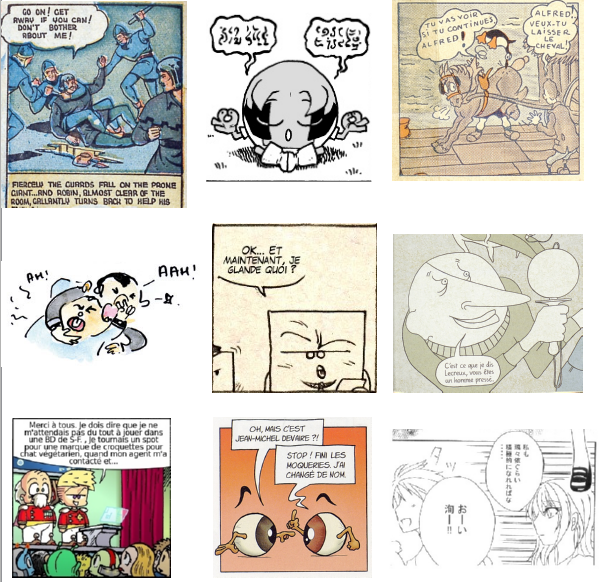
\includegraphics[trim= 4px 0px 0px 0px, clip, width=230px]{comics_diversity.png}
%   \caption[Examples of comic panels that reflect the diversity of comic books of the dataset]{Examples of comic panels that reflect the diversity of comic books of the dataset.}
%   \label{fig:ex:comics_diversity}
%  \end{figure}

% %%%%%%%%%%%%%%%%%%%%%%%%%%%%%%%%%%%%%%%%%%%%%%%%%%

It took almost one year to define which type of comics are the most interesting for researchers, meet and convince comic book authors and publishers, get copyright authorizations for the scientific community, develop a specific annotation tool and finally to hire people to manually create the ground truth.

A selection of hundred comic pages were annotated in one day by twenty volunteers affiliated to the L3i lab.
In order to provide a common basis for evaluating research work, the ground truth have been published in 2013~\cite{Guerin2013} and made available to the scientific community through a dedicated website\footnote{\url{http://ebdtheque.univ-lr.fr}}.
It has been enriched in 2014 by adding the location of the principal comic characters and semantic information to the already annotated elements.

The content of the dataset and its terms of use, the ground truth construction protocol and its quality assessment are detailed in the four next sub sections.



% \section{Structure and indexation}
% \label{sec:gt:structure_indexation}
\subsection{Dataset description} % (fold)
\label{sec:dataset_description}

% section dataset_description (end)

Scott McCloud defined comics as ``juxtaposed pictorial and other images in deliberate sequence, intended to convey information and/or to produce an aesthetic response in the viewer''~\cite{mccloud1994understanding}.
This definition is intentionally broad enough to encompass the spectrum of the majority of works produced so far.
The dataset composition should reflects this heterogeneity to give everyone the opportunity
to compare its algorithms to a globally representative dataset of the comics world.
We contacted authors with different comic styles and have selected a corpus of one hundred images, representing single or double comics page.

The images were partly processed by the French company A3DNum\footnote{\url{http://www.a3dnum.fr}} which was commissioned to digitize 14 albums.
Among all the files, scanned at a resolution of 300 dots per inch and encoded in uncompressed Portable Network Graphic (PNG) format, we used 46 pages to integrate the eBDtheque corpus.
The remaining 54 images were selected from webcomics, public domain comics\footnote{\url{http://digitalcomicmuseum.com}} and unpublished artwork with different styles from 72 to 300 dots per inch.
We encoded all the images of the eBDtheque dataset in Joint Photographic Experts Group (JPEG) format with a lossy compression to facilitate file exchange.
%, the non compressed images are available on request.

Hereafter we describe the characteristics of the selected pages and their content.


\paragraph{Albums} % (fold)
 \label{par:albums}
 The albums have been published between 1905 and 2012.
 29 pages were published before 1953 and 71 after 2000.
 Quality paper, colour saturation and textures related to printing technique changes can vary a lot from one image to another.
 The artworks are mainly from France (81\%), United States (13\%) and Japan (6\%).
 Their styles varies from classical Franco-Belgium ``bandes dessinées'' to Japanese manga through webcomic and American comics.

 % paragraph albums (end)

\paragraph{Pages} % (fold)
\label{par:pages}
The pages themselves have very diverse characteristics.
Among all, 72 are printed in colours and according to the authors and periods, there are a majority of the tint areas, watercolours and hand-coloured areas.
Among the remaining 28, 16 have are greyscale and 12 are simply black and white.
One album has two versions of each page, one in colour and the other one in black and white.
We have integrated an examples of each of them in order to allow performance comparison of algorithms on the same graphic style by using colour information or not.
Five of the 100 images are double page, others are single page and 20\% are not A4 format.
% We therefore, strictly speaking, 105 and 100 pages not in our database, each with a distinct structure
% paragraph pages (end)

\paragraph{Panels} % (fold)
\label{par:panels}
The panels contained in the pages are of various shapes.
Although most of them are bounded by a black line, a significant proportion has at least one part of the panel which is indistinguishable from the background of the page (framele panel).
Two pages consist only of frameless panels, the visual delimitation uses background contrast difference between the panel and image.
Nine images contain overlapping panels, twelve contain only panels without border and several have panels connected by a straddle object.

% paragraph panels (end)

\paragraph{Balloons} % (fold)
\label{par:balloons}
The balloons also contain a great diversity.
Some of them are completely surrounded by a black stroke, some partially and others not at all.
They have a bright background with a rectangular, oval or non geometric shape with ``smooth'', ``wavy'' or ``spiky'' contour in general.
Most of them have a tail pointing towards the speaker, but some have not.
There is text without any surrounding balloons on 33 images of the corpus.
% and 8 of them simply contain no bubble.

% paragraph balloons (end)

\paragraph{Text} % (fold)
\label{par:text}
The text is either typewritten or handwritten, mainly upper-case. % (61\% of the images are typewritten?)
The text lines contains 12 elements in average (Figure~\ref{fig:ex:textline_lenth_distribution}) and there are more than hundred text lines that are composed by only one letter corresponding to punctuation or single letter words such as ``I'' or ``A''; this is a particularity of comics.

Most pages are from French artworks, where the text is written in French.
Only 13 pages contain English text and 6 images are in Japanese.
Onomatopoeia appears in 18 pages.

    %%%%%%%%%%%%%%%%%%%%%%%%%%%%%%%%%%%%%%%%%%%%%%%%%%%%%%%%
    \begin{figure}[ht]%trim=l b r t  width=0.5\textwidth,  
      \centering
      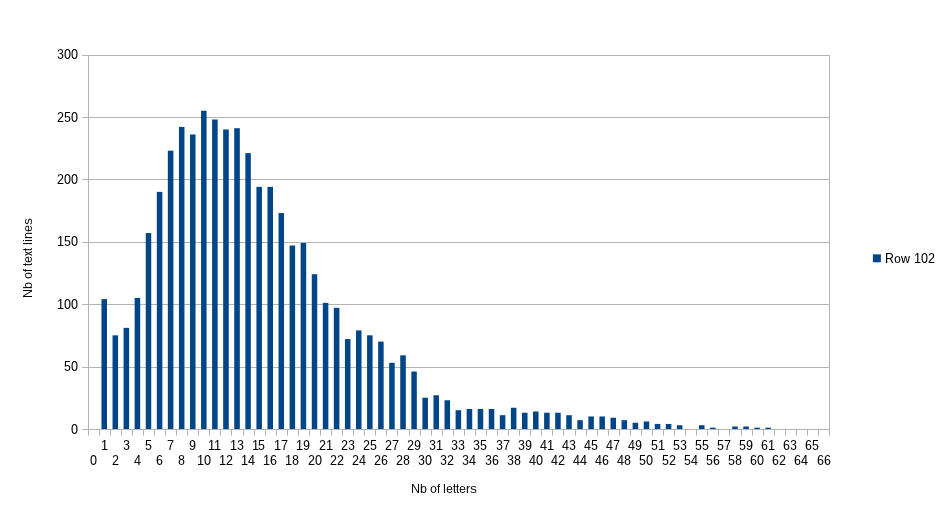
\includegraphics[trim= 0px 5px 65px 5px, clip, width=0.85\textwidth]{number_of_letter_per_textline.png}
      \caption[Distribution of the number of elements per text lines]{Distribution of the number of elements per text lines.
      }
      \label{fig:ex:textline_lenth_distribution}
    \end{figure}  
    %%%%%%%%%%%%%%%%%%%%%%%%%%%%%%%%%%%%%%%%%%%%%%%%%%%%%%%%

% paragraph text (end)

\paragraph{Comic characters} % (fold)
\label{par:comic_characters}
The comic characters or protagonists are specific to each album.
They all have eye, harm and leg but at least 50\% are not humanoid, depending on the interpretation.
% paragraph comic_characters (end)

% DATASET FULL DESCRIPTION MOVED TO APPENDIX 2014-09-18

\subsection{Ground truth information} % (fold)
\label{sub:ground_truth}

We give all the details about the ground truth construction process in Appendix~\ref{app:groundtruth}.
The annotation of visual information such as the location of panels, balloons, text lines and comic characters is detailed.
Also, present the annotation of semantic information about the type of text, relationship between speech balloons and speaking characters; and bibliographic information about the images (e.g. page number, author, ISBN, release date).
Finally, the file structure, the annotation quality assessment and the terms of use are defined.

% subsection ground_truth (end)

% \subsection{Discussions}
% \label{ssec:gt:siscussions}

% We presented the eBDtheque dataset, the first comic image dataset and associated ground truth on comic books containing spatial and semantic annotations, publicly available for the scientific community.
% % The corpus has been introduced as well as the construction protocol.
% The corpus can be extended to enlarge the diversity of the dataset and provide consecutive page or full album in order to allow a wider level of comic books analysis.
% New semantic annotations can be added, such as the view angle and the shot type for panels, text at the level of letters, comic character's role, profile and relationships. 


% section dataset_and_ground_truth_construction (end)

\section{Metrics} % (fold)
\label{sec:ex:metrics}
The contributions of this thesis are from different nature and need to be evaluated separately using appropriate metrics.
Object localisation developments are evaluated using the commonly used recall and precision metrics and other contributions are evaluated using accuracy.

\subsection{Object localisation metric} % (fold)
\label{sub:ex:object_localisation_metric}


% paragraph metrics (end)
We evaluate the different extractions (panel, balloon and text regions) in terms of object bounding boxes such as the PASCAL VOC challenge~\cite{everingham2010pascal}.
The detections are assigned to ground truth objects and judged to be true or false positives by measuring bounding box overlap.
To be considered as a correct detection, the overlap ratio $a_0$ between the predicted bounding box $B_p$ and the ground truth bounding box $B_{gt}$ (Formula~\ref{eq:ex:overlap_ratio}) must exceed 0.5.
The predicted objects are considered as true positive $TP$ if $a_0 > 0.5$ or false positive $FP$ (prediction errors) otherwise.

\begin{equation}
\label{eq:ex:overlap_ratio}
  a_0 = \frac{area(B_p \cap B_{gt})}{area(B_p \cup B_{gt})}
\end{equation}

Detections returned by a method are assigned to ground truth objects satisfying the overlap criterion ranked by the confidence output (decreasing).
Multiple detections of the same object in an image are considered as false detections (e.g. 5 detections of a single object counted as 1 correct detection and 4 false detections).

The number of $TP$, $FP$ and false negative (missed elements) $FN$ are used to compute the recall $R$, precision $P$ and F-measure $F$ of each method using Formulas~\ref{eq:ex:recall_precision}.
% We also compute the F-measure $F$ for each result.

\begin{align}
\label{eq:ex:recall_precision}
R = \frac{TP}{TP + FN} && P = \frac{TP}{TP + FP} && F = 2 * \frac{P * R}{P + R}
\end{align}

% \begin{equation}
% \label{eq:recall}
%   R = \frac{TP}{TP + FN}
% \end{equation}
% % where $FN$ is the number of false negative (missed elements).

% \begin{equation}
% \label{eq:precision}
%   P = \frac{TP}{TP + FP}
% \end{equation}
% where $FP$ is the number of false positives (prediction errors).


\subsection{Object segmentation metric} % (fold)
\label{sub:ex:object_segmentation_metric}

Object bounding box based evaluation is appropriate for surface comparison but not for detailed region extraction evaluation.
In Section~\ref{sub:in:balloon_classification} we extract balloon contour at the level of pixel for analysis and classification purposes.
In order to make the difference between the errors sources we need to use a more precise evaluation framework.
Here we keep using recall and precision metrics as introduced in the previous section but instead of counting the number of objects that valid a certain criterion, we simply count the number of pixels that have been detected correctly ($TP$), incorrectly ($FP$) or missed ($FN$).


\subsection{Text recognition metric} % (fold)
\label{sub:ex:text_recognition_metric}
Even if text recognition would require more investigation to be fully treated, we give a first baseline evaluation in Section~\ref{par:ex:text_recognition_evaluation} using commercial OCR systems on the eBDtheque dataset.
We evaluated the text detection accuracy $A_{textReco}$ at a given string edit distance between the predicted recognition and its corresponding transcription in the ground truth~\cite{Guerin2013}.

% subsection text_recognition (end)

% subsection object_localisation (end)
\subsection{Tail detection metric} % (fold)
\label{sub:ex:tail_detection_metric}
% We evaluated the proposed tail extraction method on the 1092 balloons of the eBDtheque dataset~\cite{Guerin2013} ``version 2014''.
% In the ground truth, some balloons do not have a tail but we did not remove them as the proposed method can also detect when there is no tail and return a correct answer.

Tail tip and tail direction are not surfaces, therefore they can not be evaluated using recall and precision metrics presented Section~\ref{sub:ex:object_localisation_metric}.
%+For this particular case, we redefine the recall and precision by measuring the Euclidean distance between the detected tip and its ground truth (recall) and the direction error (precision).
Thus, we define two accuracy metrics $A_{tailTip}$, the accuracy of the predicted position of the tail tip and $A_{tailDir}$ the accuracy of the tail direction prediction.
The Euclidean distance $d_0$ between the predicted position of the tip and its ground truth is measured relative to balloon size (Formula~\ref{eq:ex:accuracy_tailtip}).
Note that we consider as incorrect the predicted positions at a distance $d_0$ superior to the balloon size ($A_{tailTip} < 0$). 

\begin{equation}
\label{eq:ex:accuracy_tailtip}
  A_{tailTip} = 1 - \frac{d_0}{0.5 * (B_{width} + B_{height})}
\end{equation}
where $B_{width}$ and $B_{height}$ correspond to the balloon width and height respectively.
 % as follow $A_{tailTip} = 1 - d_0/ (B_{width} + B_{height})/2 )$.

The direction accuracy $A_{tailDir}$ was measured according to the distance $d_1$ within the eight cardinal coordinate sequences defined in Section~\ref{tab:se:offset_panel_corner} (Formula~\ref{eq:ex:accuracy_taildir}).

\begin{equation}
\label{eq:ex:accuracy_taildir}
  A_{tailDir} = 1- \frac{d_1}{8}
\end{equation}

For instance if the detected direction was $S$ (south) and the ground truth was $SE$ (south-east) then $d_1=1$.
Note that our method can also detect when there is no tail on the balloon contour $C_{tail}=0\%$ (confidence equal to zero percent); in this case $A_{tailTip}=A_{tailDir}=100\%$ if there was effectively no tail to detect or $A_{tailTip}=A_{tailDir}=0\%$.
% For this experiment, the local window size $M$ of the tail direction process was set to 10\% of the mean balloon size (Equation~\ref{eq:se:mean_balloon_size}) in order to be invariant to the image definition \modif{TODO: justify}.

% subsection tail_detection (end)

\subsection{Semantic links metric} % (fold)
\label{sub:ex:semantic_links_metric}

The semantic links between speech text and speech balloon are called $STSB$ and the ones between speech balloon and speaking character $SBSC$; they characterise a dialogue.
They are considered true or false according to their existence or not in the ground truth.
We evaluated the semantic relations $STSB$ and $SBSC$ according to the metadata in the ground truth of the eBDtheque dataset~\cite{Guerin2013} called \texttt{{isLineOf}} and \texttt{{isSaidBy}}, which represent 3427 and 829 relations respectively.
We defined two accuracy metrics $A_{STSB}$ and $A_{SBSC}$ to measure the percentage of correctly predicted semantic links (Formula~\ref{eq:ex:accuracy_semantic_links}).

\begin{align}
\label{eq:ex:accuracy_semantic_links}
A_{STSB} = \frac{nbRetrievedSTSBLinks}{nbSTSBLinks} && A_{SBSC} = \frac{nbRetrievedSBSCLinks}{nbSBSCLinks}
\end{align}

% subsection semantic_links_and_text_recognition (end)

% section metrics (end)

% \section{Parameter validation}

% \section{Evaluation} % (fold)
% \label{sec:ex:evaluation}

% We evaluate the contributions of the thesis at different levels.
% We first evaluate the sequential, independent and knowledge-driven approaches separately and then we compare them in the global evaluation section.

% \section{Sequential information extraction evaluation} % (fold) %IJDAR
% \label{sub:ex:sequential_information_extraction_evaluation}

% TODO

\section{Panel extraction evaluation} % (fold)
\label{sub:ex:panel_extraction_evaluation}
% We evaluated the proposed method on the 850 panels of the eBDtheque dataset~\cite{Guerin2013} ``version 2014'' at bounding box level.

In this section we evaluate our three approaches \modif{(Method S, I and K)} and compare them to two methods from the literature.
We compare our results to Arai~\cite{Arai10} and Ho~\cite{Ho2012} that are two state of the art methods (Section~\ref{sec:sota:layout_panel}).
The first one use connected-component analysis similarly to our proposition and the second is based on growing region.

All the evaluations are performed on the 850 panels of the eBDtheque dataset (Section~\ref{sec:dataset_and_ground_truth_construction}) at object bounding box level, using the recall and precision metrics introduced in Section~\ref{sub:ex:object_localisation_metric}.

% \subsection{Experimental settings} % (fold)
% \label{sub:experimental_settings}

% TODO

\subsection{Arai's method} % (fold)
\label{sub:ex:panel_extraction_arai}
We have implemented the comic panel extraction method presented in~\cite{Arai10} except the division line detection by lack of detail in the original paper.

This method consists in a bi-level segmentation with an empiric threshold value of 250 followed by a connected-component extraction, binary image inversion and blob selection.
The final blob selection is based on a minimal size of $Image.Width / 6$ and $Image.Height / 8$.
From the selected blobs, a line detection approach is applied as final decision.
This line detection approach is able to cut overlapped panels on a page size basis which is appropriate for pages with a single panel per strip as illustrated Figure~\ref{fig:ex:division_line_detection}.
The author did not share the code and we were not able to re implement this part by lack of detail in the original paper.
Anyway, the line division method works only for panels that are as large as the page which is not so common and would not have affected the result significantly (Figure~\ref{fig:ex:division_line_detection}).

%%%%%%%%%%%%%%%%%%%%%%%%%%%%%%%%%%%%%%%%%%%%%
\begin{figure}[h!]
\begin{center}
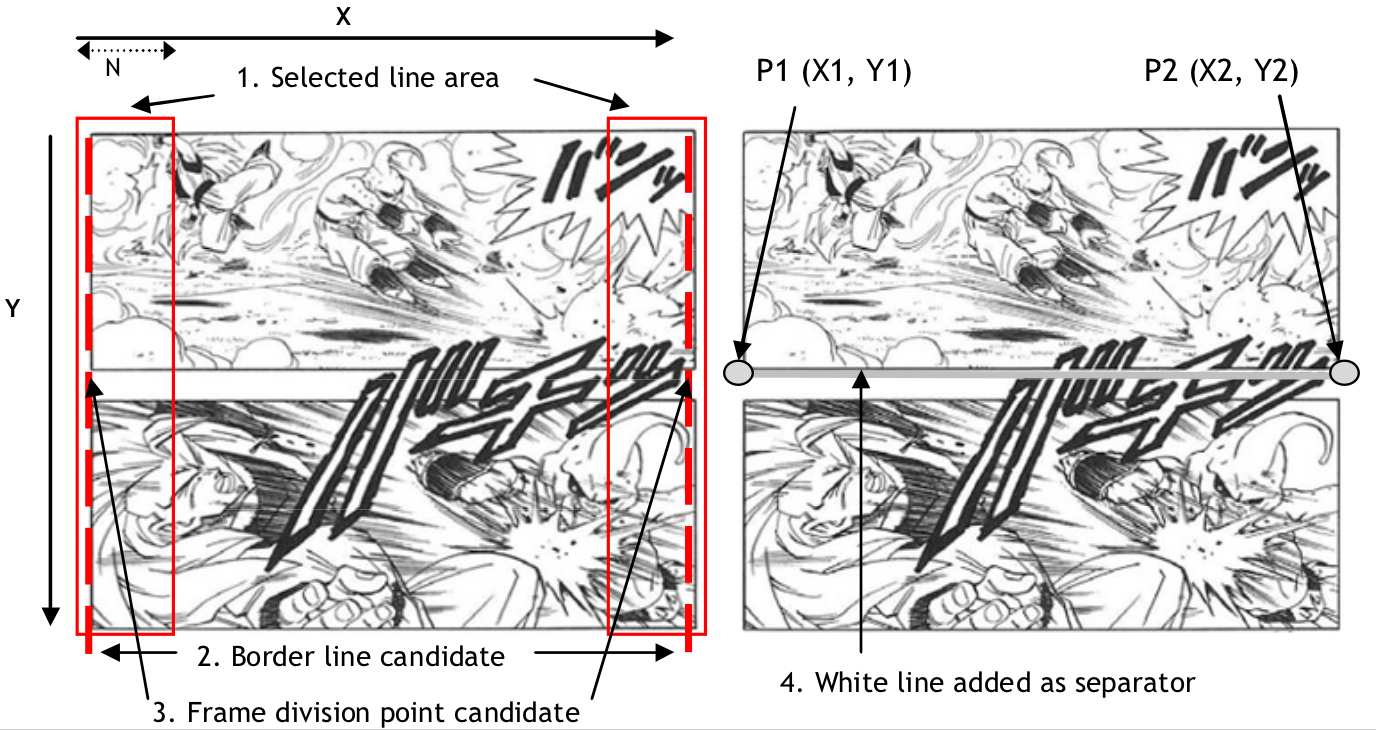
\includegraphics[width=0.8\textwidth]{division_line_detection_arai10.png}
\caption[Division line detection for panel extraction]{Division line detection from~\cite{Arai10} (figure 5 in the author's paper).}
\label{fig:ex:division_line_detection}
\end{center}
\end{figure}
%%%%%%%%%%%%%%%%%%%%%%%%%%%%%%%%%%%%%%%%%%%%%

The score of this method was in average for recall and precision of 20.00\% and 18.75\% (Figure~\ref{fig:ex:panel_arai_extraction_detail}).

%%%%%%%%%%%%%%%%%%%%%%%%%%%%%%%%%%%%%%%%%%%%%%%%%%%%%%
% \begin{figure}
%  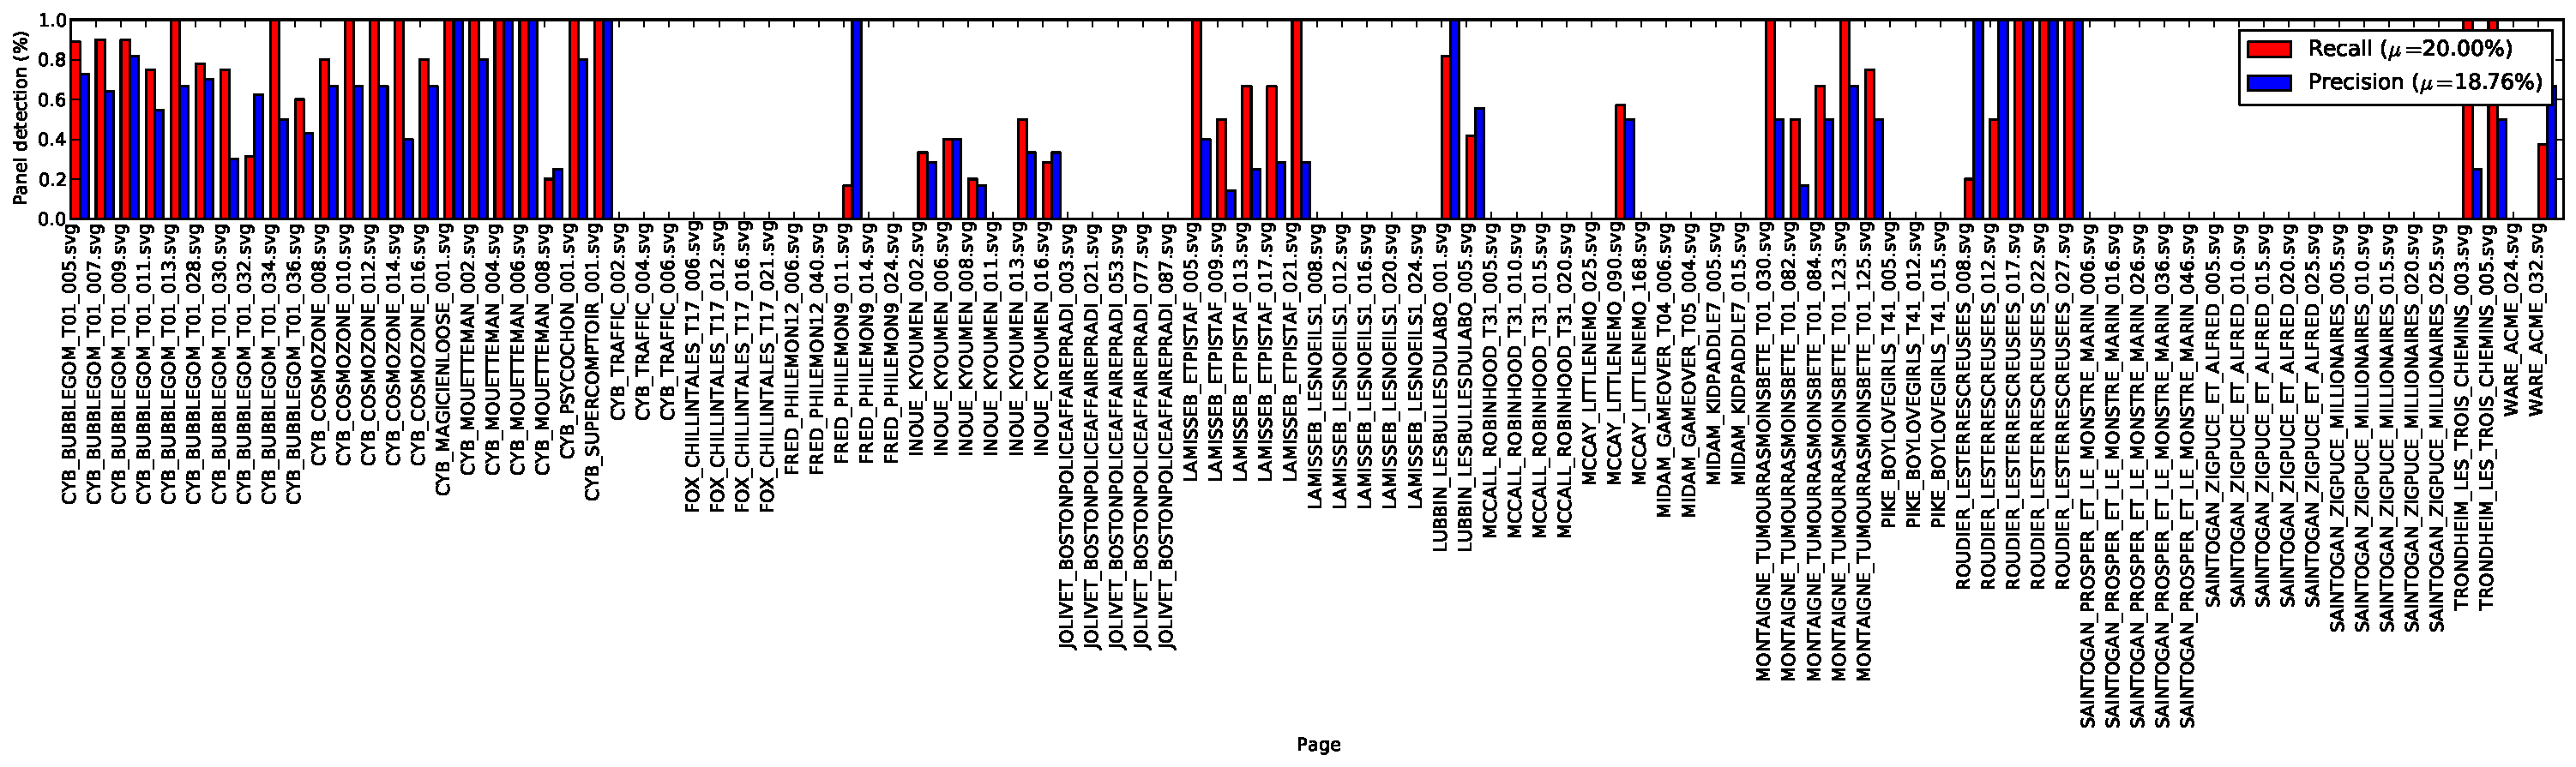
\includegraphics[width=\textwidth,height=4cm]{2014-07-20_svg_Arai2010_no_division_linePanel_object.pdf}
%  \caption{Panel extraction score details for each image of the eBDtheque dataset (Appendix~\ref{app:dataset}).
%  }
%  \label{fig:ex:panel_arai_extraction_detail}
% \end{figure}
%%%%%%%%%%%%%%%%%%%%%%%%%%%%%%%%%%%%%%%%%%%%%%%%%%%%%%


% subsection arai_cite_arai (end)

\subsection{Ho's method} % (fold)
We have implemented the Ho's method~\cite{Ho2012} with the original parameters and set the minimal and maximal lower brightness difference of the region growing method to 20 (not mentioned in the original paper).
The image border is filled with the average five-pixel page border colour and four seeds are initialized on the four corners of the image.
When the region growing algorithm stops, the background is removed which separated panel blocks.
Mathematical morphology (dilatation) is then applied until blocks become smaller than $1/6$ of the page size and then the same number of erosion is applied in order to give back to the objects their initial size.
This manipulation separates the connected panels but has the disadvantage of creating unwanted holes as well (Figure~\ref{fig:ex:panel_ho_extraction_process}).

%%%%%%%%%%%%%%%%%%%%%%%%%%%%%%%%%%%%%%%%%%%%%%%%%%%
\begin{figure}[!ht] %trim=l b r t  width=0.5\textwidth, 
  \centering
  %\includegraphics[height=60mm]{figure/BUBBLEGOM_T01_P007_crop.jpg}
  %\includegraphics[trim= 0mm 0mm 0mm 0mm]{figure/BUBBLEGOM_T01_P007.jpg}
  \subfloat[Original image]{\label{fig:ex:se:panel_ho_img}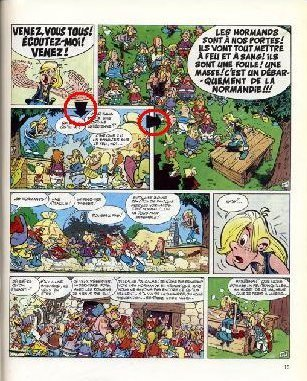
\includegraphics[trim= 0mm 0mm 0mm 0mm, clip, width=0.2\textwidth]{ho01.png}}
  \hspace{1em}
  \subfloat[Binary segmentation]{\label{fig:se:panel_ho_binary}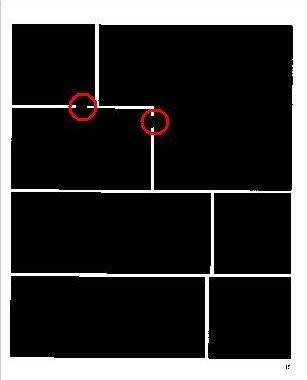
\includegraphics[trim= 0mm 0mm 0mm 0mm, clip, width=0.2\textwidth]{ho02.png}}
  \hspace{1em}
  \subfloat[After dilatation step]{\label{fig:ex:panel_ho_dilate}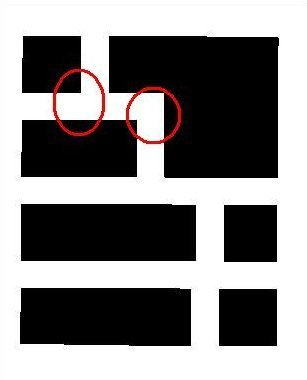
\includegraphics[trim= 0mm 0mm 0mm 0mm, clip, width=0.2\textwidth]{ho03.png}}
  \subfloat[After erosion step]{\label{fig:ex:panel_ho_erode}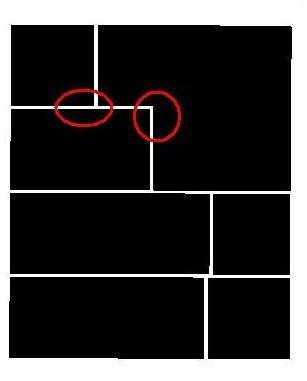
\includegraphics[trim= 0mm 0mm 0mm 0mm, clip, width=0.2\textwidth]{ho04.png}}  
    \caption[Panel extraction process of Ho]{Panel extraction and separation process of Ho~\cite{Ho2012}.}
    \label{fig:ex:panel_ho_extraction_process}
\end{figure}
%%%%%%%%%%%%%%%%%%%%%%%%%%%%%%%%%%%%%%%%%%%%%%%%%%%

The score of this method was in average for recall and precision of 49.76\% and 68.74\% (Figure~\ref{fig:ex:panel_ho_extraction_detail}).

%%%%%%%%%%%%%%%%%%%%%%%%%%%%%%%%%%%%%%%%%%%%%%%%%%%%%%
% \begin{figure}
%  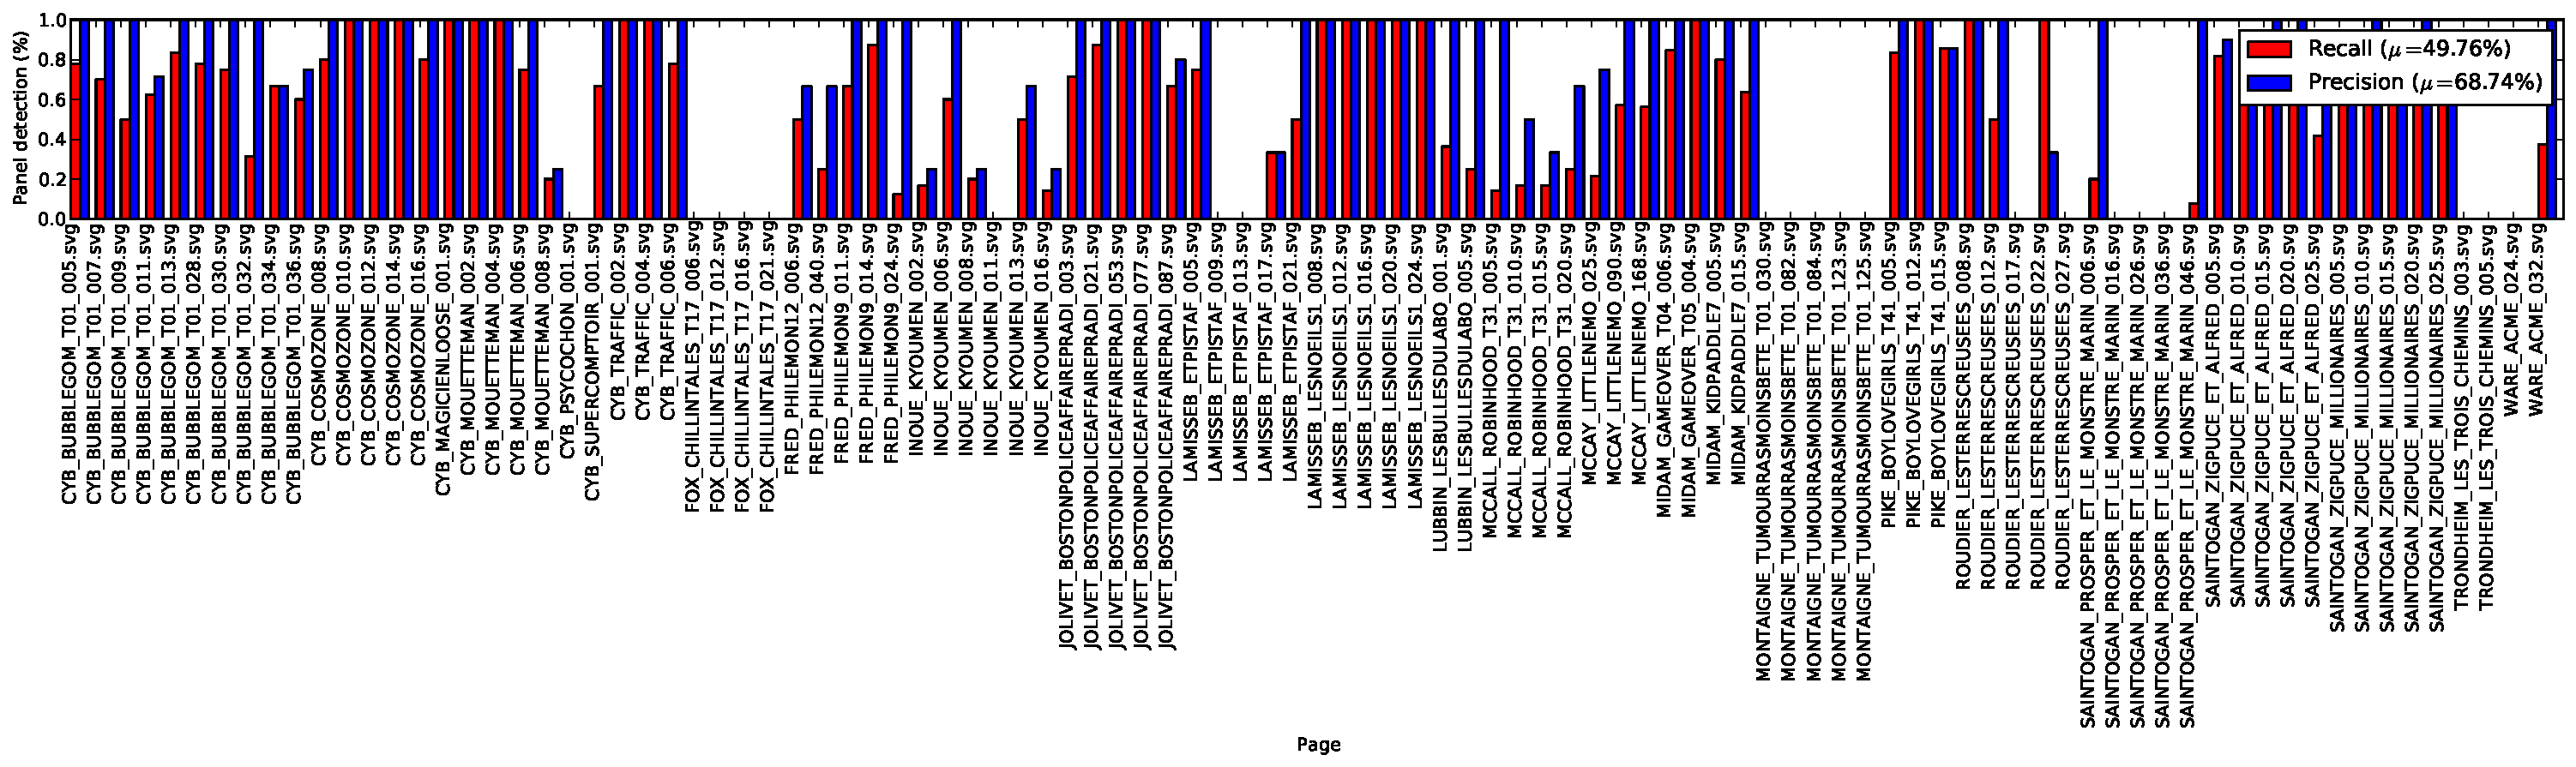
\includegraphics[width=\textwidth,height=4cm]{2014-07-20_svg_Ho2012Panel_object.pdf}
%  \caption{Panel extraction score details for each image of the eBDtheque dataset (Appendix~\ref{app:dataset}).
%  }
%  \label{fig:ex:panel_ho_extraction_detail}
% \end{figure}
%%%%%%%%%%%%%%%%%%%%%%%%%%%%%%%%%%%%%%%%%%%%%%%%%%%%%%

\subsection{Sequential approach} % (fold)
\label{sub:ex:panel_extraction_rigaud_method_A}

The method presented in Section~\ref{sec:se:panel_and_text} is parameter free except for the number of cluster for k-means clustering algorithm that we fixed to $k=3$ for the reason explained in the presentation of the method (Section~\ref{sec:se:panel_and_text}).
Note that the method also extract text region at the same time which does not interfere with panel (Section~\ref{sub:ex:text_extraction_recognition_evaluation}).
The score of this method  was in average for recall and precision of 64.24\% and 83.81\% (Figure~\ref{fig:ex:panel_methodA_extraction_detail}).

%%%%%%%%%%%%%%%%%%%%%%%%%%%%%%%%%%%%%%%%%%%%%%%%%%%%%%
% \begin{figure}[h]
%  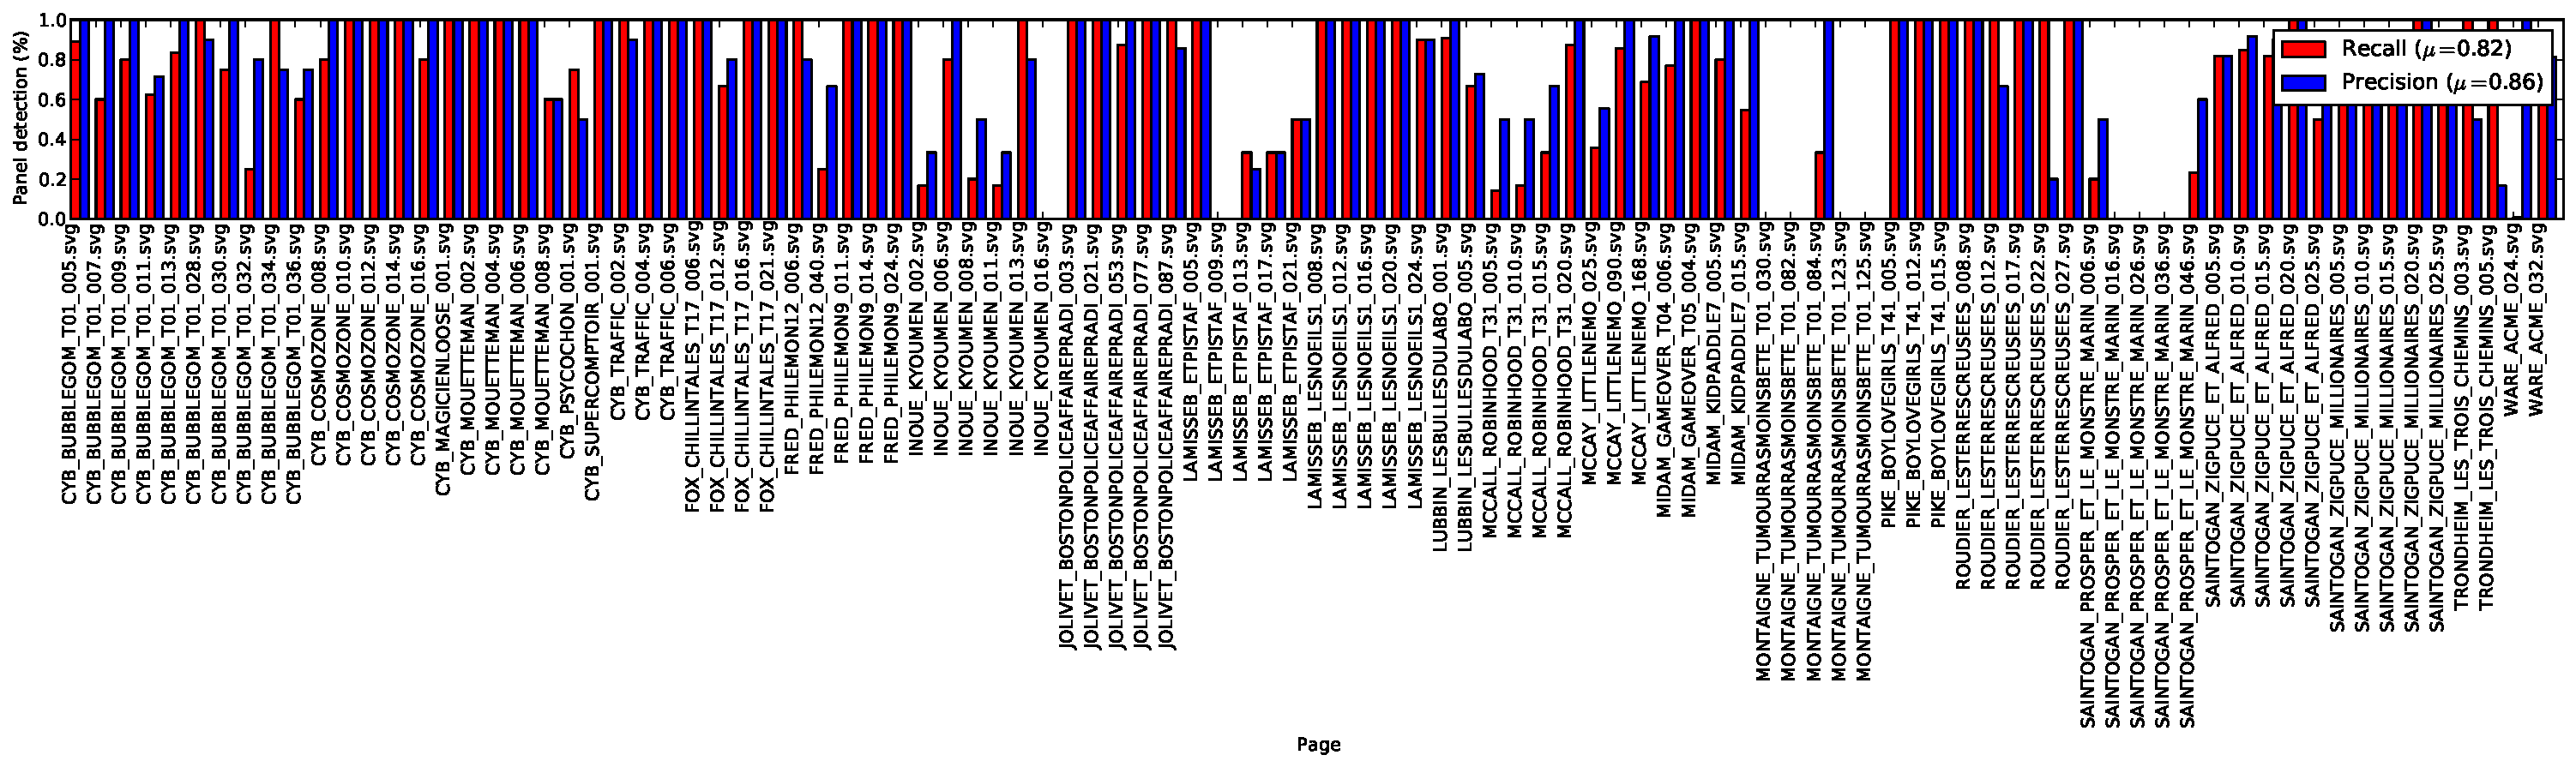
\includegraphics[width=\textwidth,height=4cm]{Panel_object_proposed.pdf}
%  \caption{Panel extraction score details for each image of the eBDtheque dataset \modif{TODO: update}.
%  }
%  \label{fig:ex:panel_methodA_extraction_detail}
% \end{figure}
%%%%%%%%%%%%%%%%%%%%%%%%%%%%%%%%%%%%%%%%%%%%%%%%%%%%%%

\subsection{Independent approach} % (fold)
% \label{sub:method_b}
The method presented in Section~\ref{sec:in:panel_extraction} requires only a minimal area factor.
Assuming that a panel is a big region, we ignored the panel detection with a area lower than 4\% ($minAreaFactor$) of the page area according to a validation on the eBDtheque dataset.
This parameter avoids to consider small and isolated elements (e.g text, logo, page number) as panel.
The score of this method was in average for recall and precision of 62.94\% and 87.30\% (Figure~\ref{fig:ex:panel_methodB_extraction_detail}).

%%%%%%%%%%%%%%%%%%%%%%%%%%%%%%%%%%%%%%%%%%%%%%%%%%%%%%
% \begin{figure}[h]
%  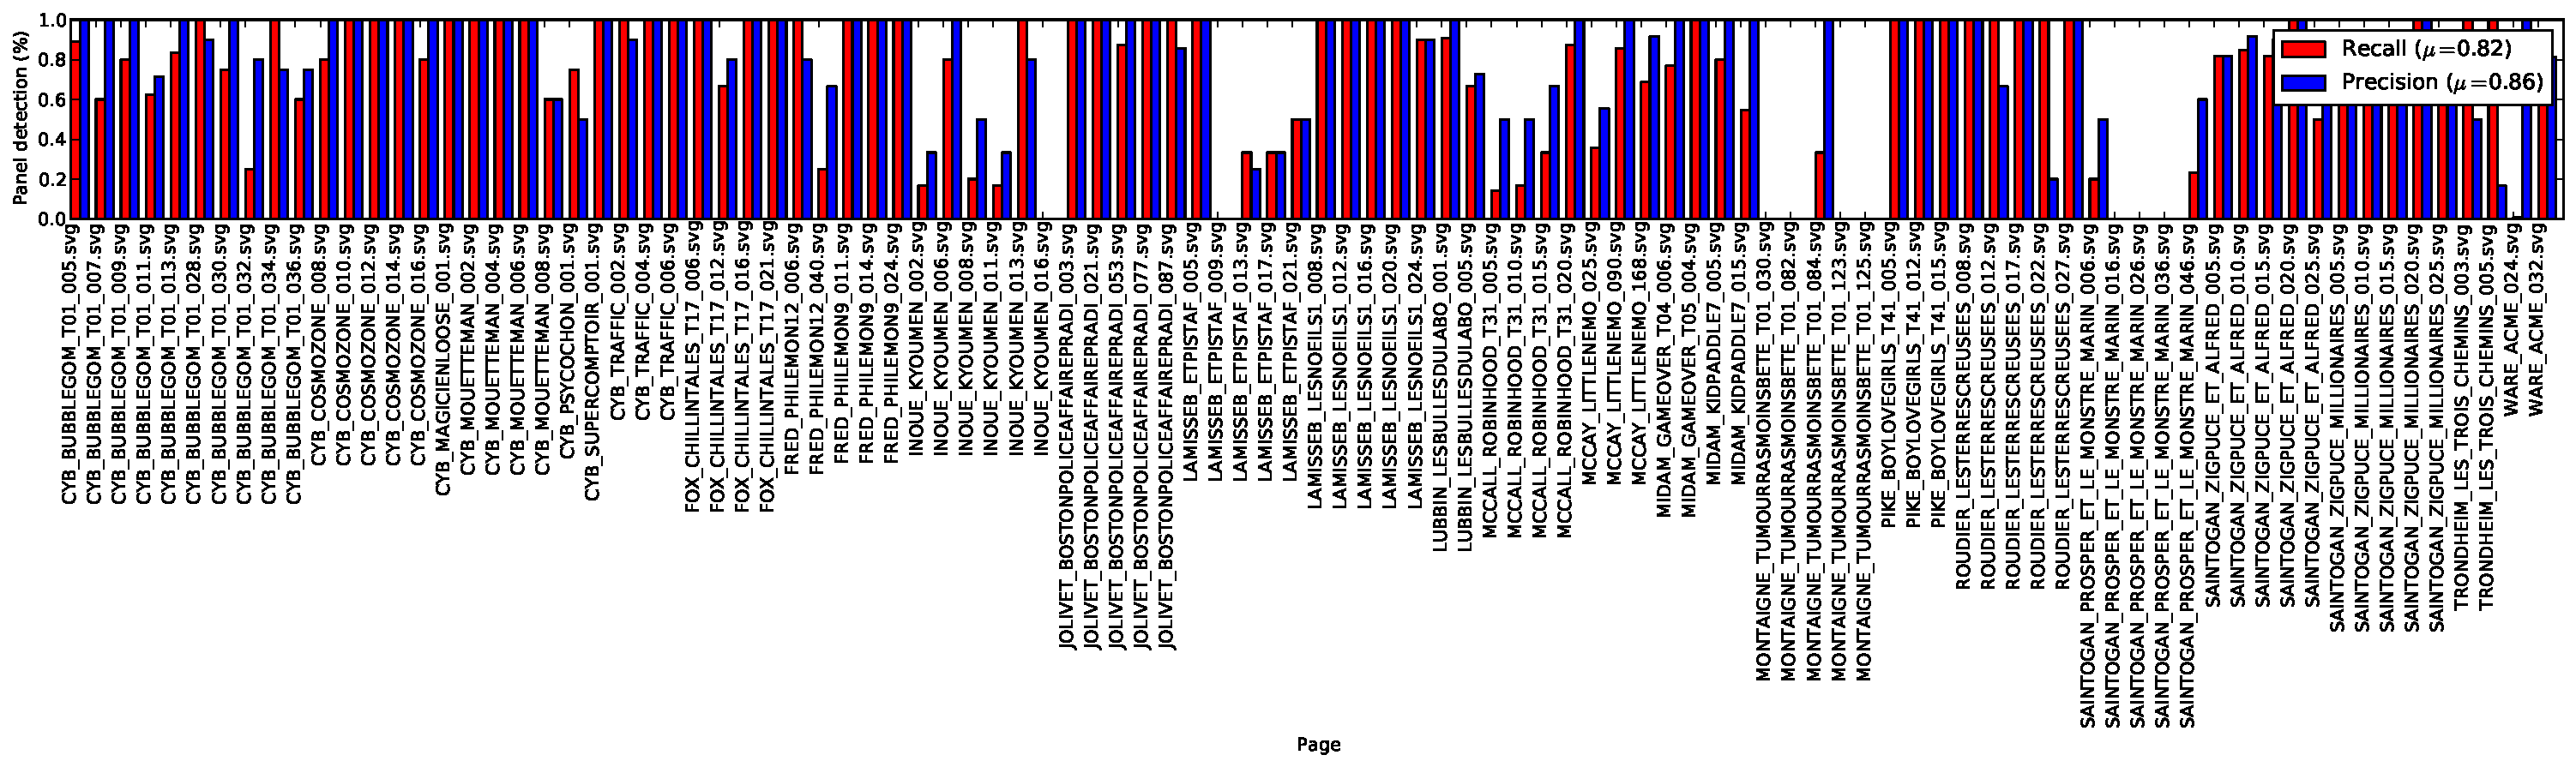
\includegraphics[width=\textwidth,height=4cm]{Panel_object_proposed.pdf}
%  \caption{Panel extraction score details for each image of the eBDtheque dataset \modif{TODO: update}.
%  }
%  \label{fig:ex:panel_methodB_extraction_detail}
% \end{figure}
%%%%%%%%%%%%%%%%%%%%%%%%%%%%%%%%%%%%%%%%%%%%%%%%%%%%%%

% subsection method_b (end)

\subsection{Knowledge-driven approach} % (fold)
% \label{sub:method_c}
The knowledge-driven method can be used as a post processing of the panel extraction.
It validates or rejects panel candidates using the proposed model (Section~\ref{sec:kn:processing_sequence}).
In the model, the only rule about the panel is that they should be contained in a image.
The score of this method for the independent panel extraction (Method I) was in average for recall and precision of 61.88\% and 87.42\% (Figure~\ref{fig:ex:panel_methodC_extraction_detail}).

% %%%%%%%%%%%%%%%%%%%%%%%%%%%%%%%%%%%%%%%%%%%%%%%%%%%%%%
% \begin{figure}[h]
%  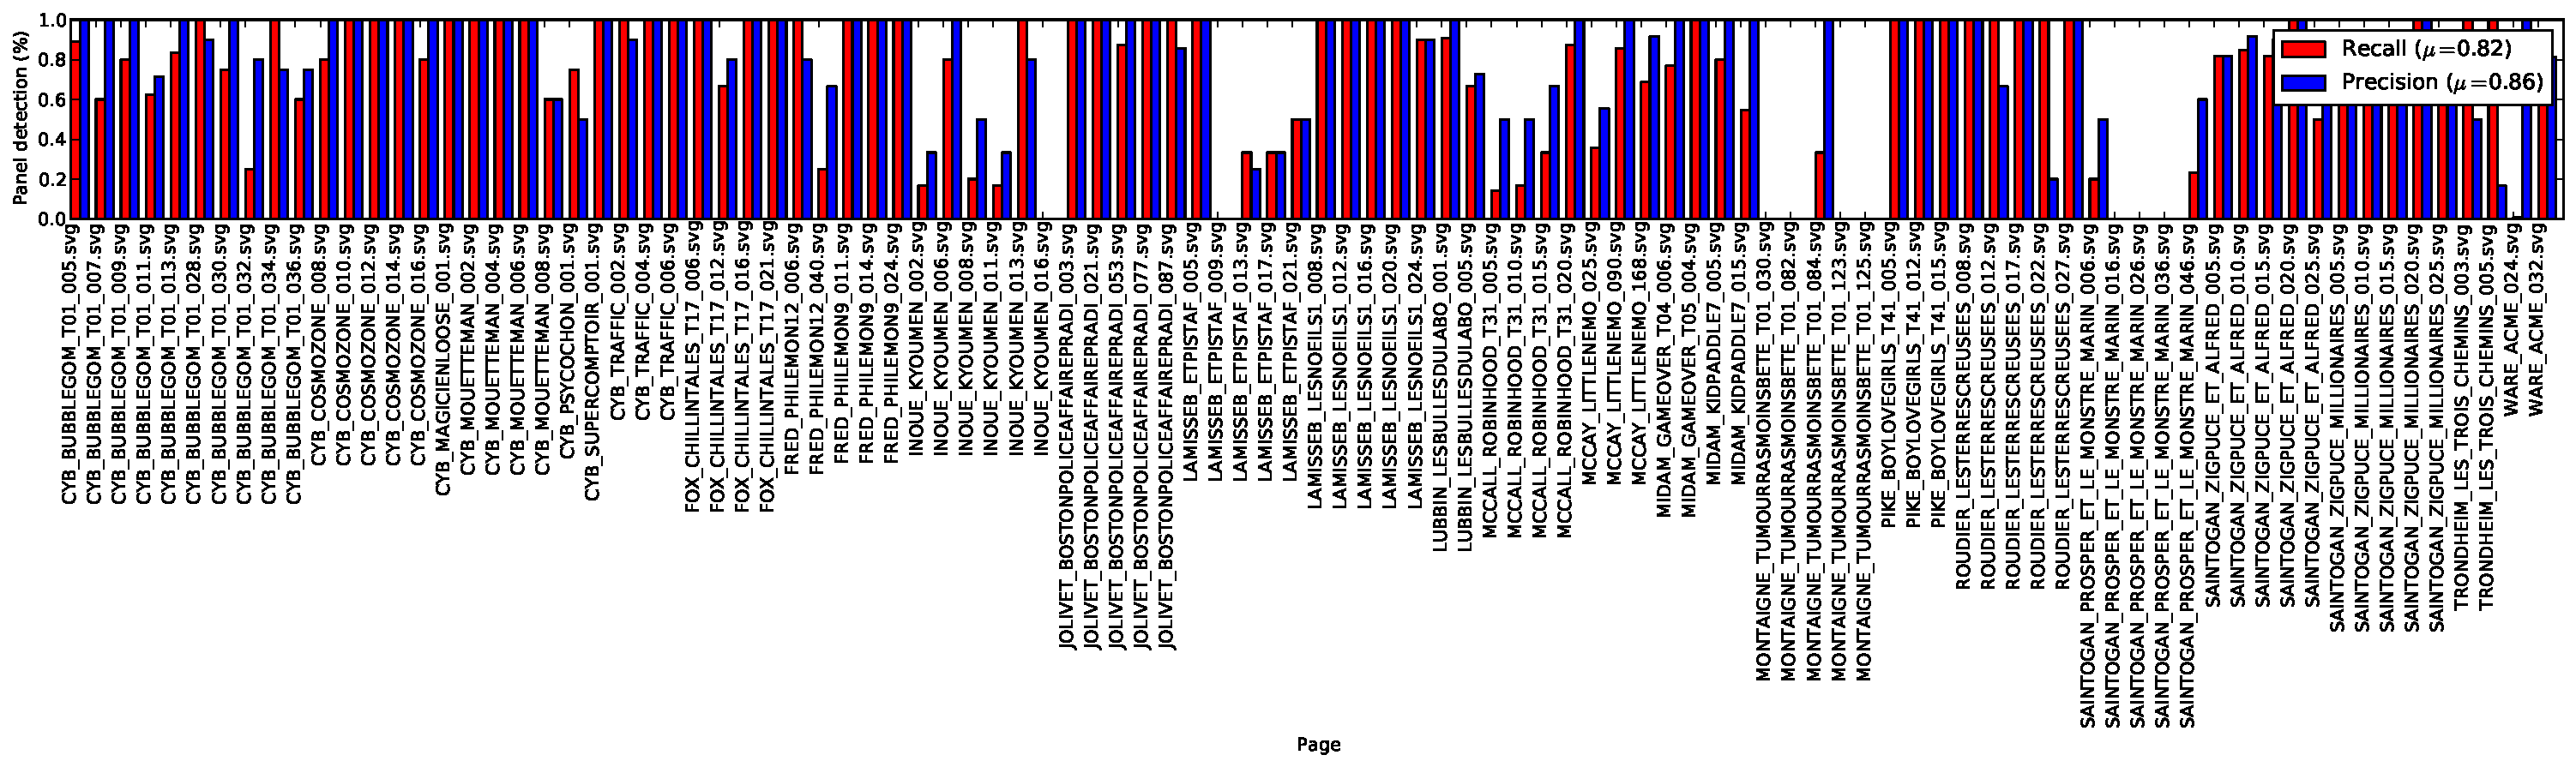
\includegraphics[width=\textwidth,height=4cm]{Panel_object_proposed.pdf}
%  \caption{Panel extraction score details for each image of the eBDtheque dataset \modif{TODO: update}.
%  }
%  \label{fig:ex:panel_methodC_extraction_detail}
% \end{figure}
%%%%%%%%%%%%%%%%%%%%%%%%%%%%%%%%%%%%%%%%%%%%%%%%%%%%%%
% subsection method_c (end)


%%%%%%%%%%%%%%%%%%%%%%%%%%%%%%%%%%%%%%%%%%%%%%%%%%%
\begin{figure}[!ht] %trim=l b r t  width=0.5\textwidth, 
  \centering
  %\includegraphics[height=60mm]{figure/BUBBLEGOM_T01_P007_crop.jpg}
  %\includegraphics[trim= 0mm 0mm 0mm 0mm]{figure/BUBBLEGOM_T01_P007.jpg}
  \subfloat[Arai's method]{\label{fig:ex:panel_arai_extraction_detail}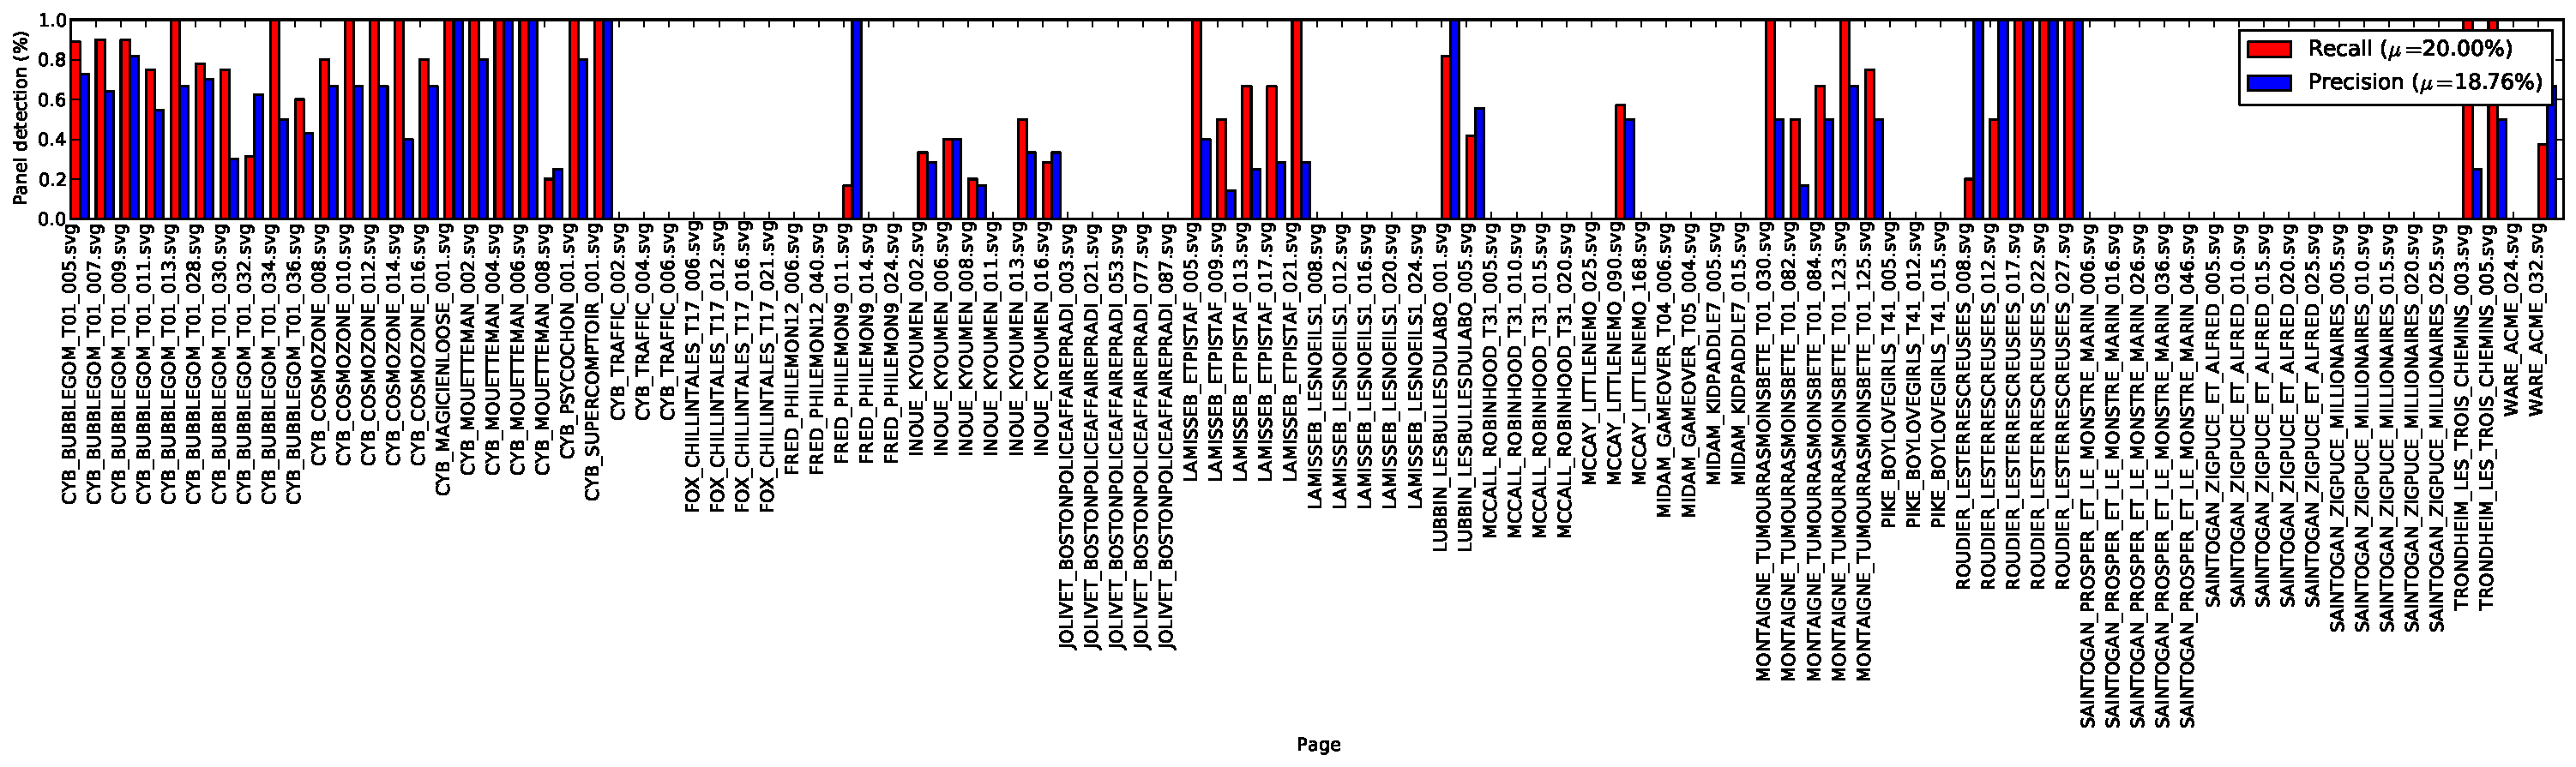
\includegraphics[trim= 0mm 108mm 0mm 0mm, clip, width=\textwidth]{2014-07-20_svg_Arai2010_no_division_linePanel_object.pdf}}
  %\hspace{1em}
  \\
  \subfloat[Ho's method]{\label{fig:ex:panel_ho_extraction_detail}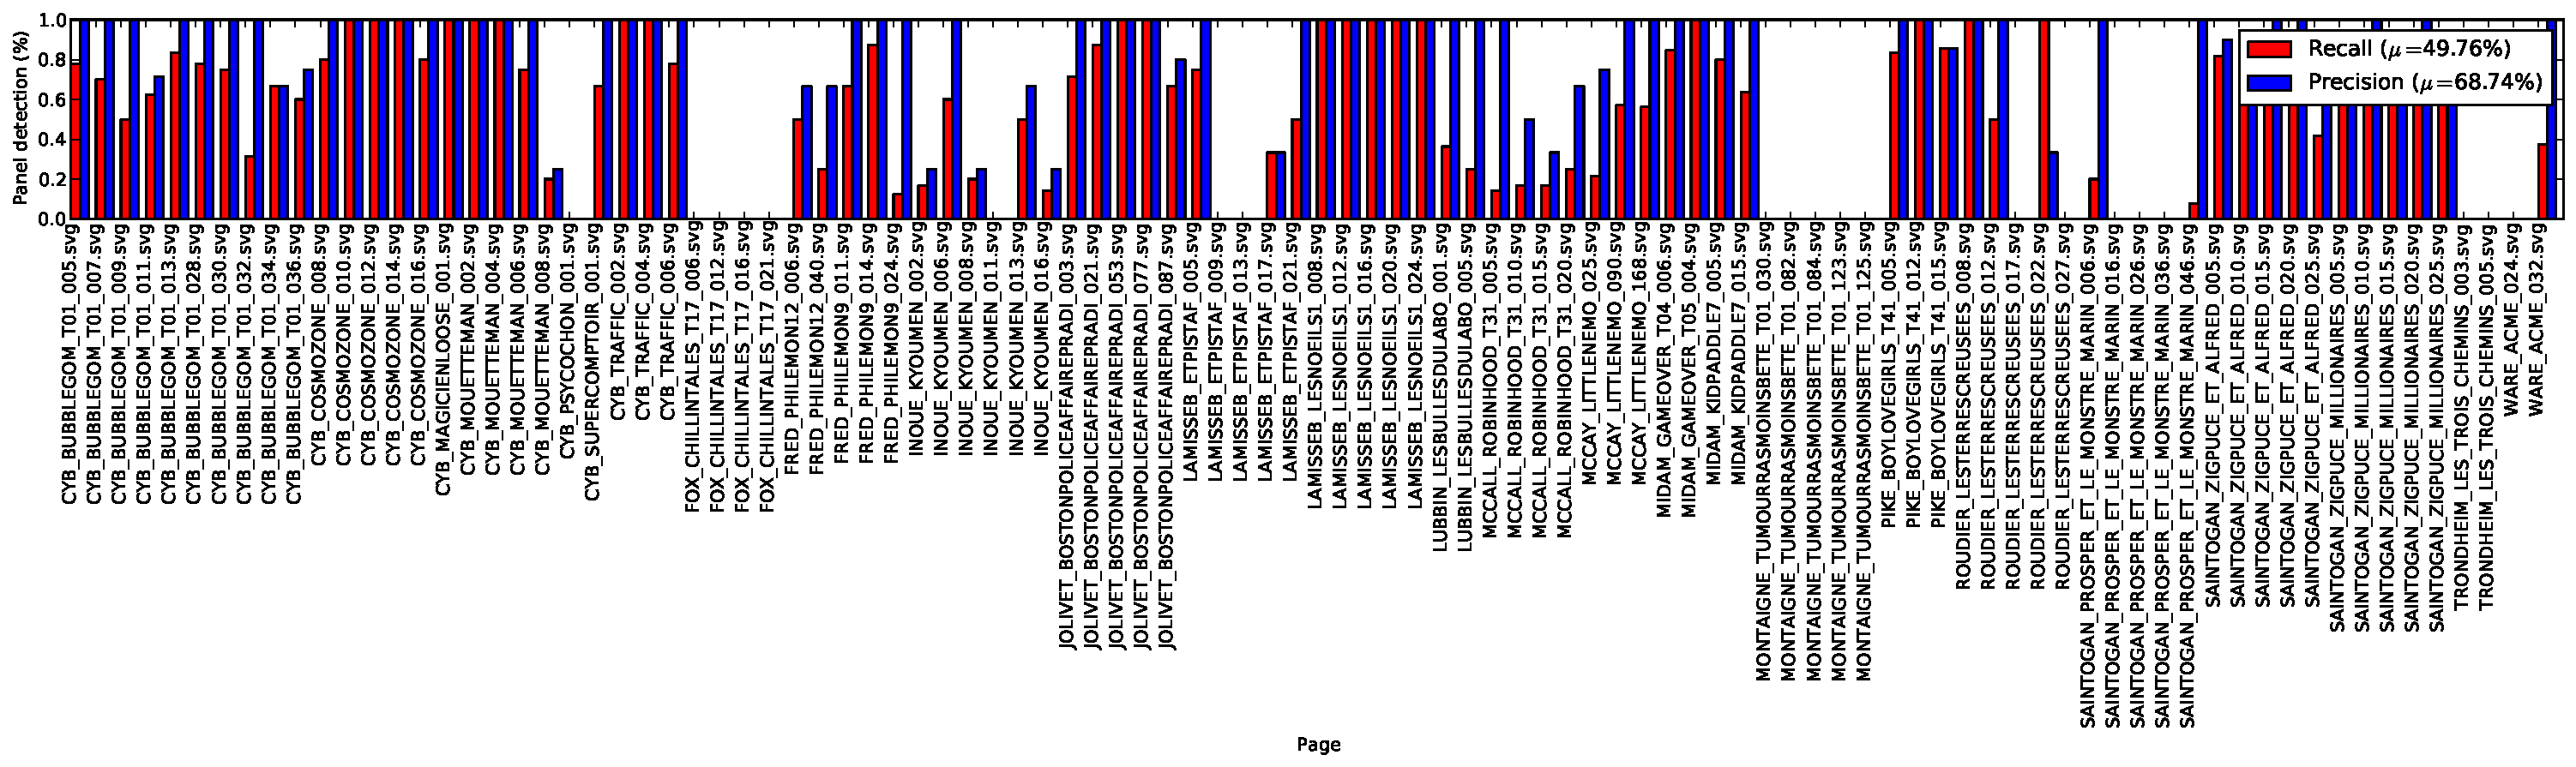
\includegraphics[trim= 0mm 108mm 0mm 0mm, clip, width=\textwidth]{2014-07-20_svg_Ho2012Panel_object.pdf}}
  %\hspace{1em}
  \\
  \subfloat[Method S]{\label{fig:ex:panel_methodA_extraction_detail}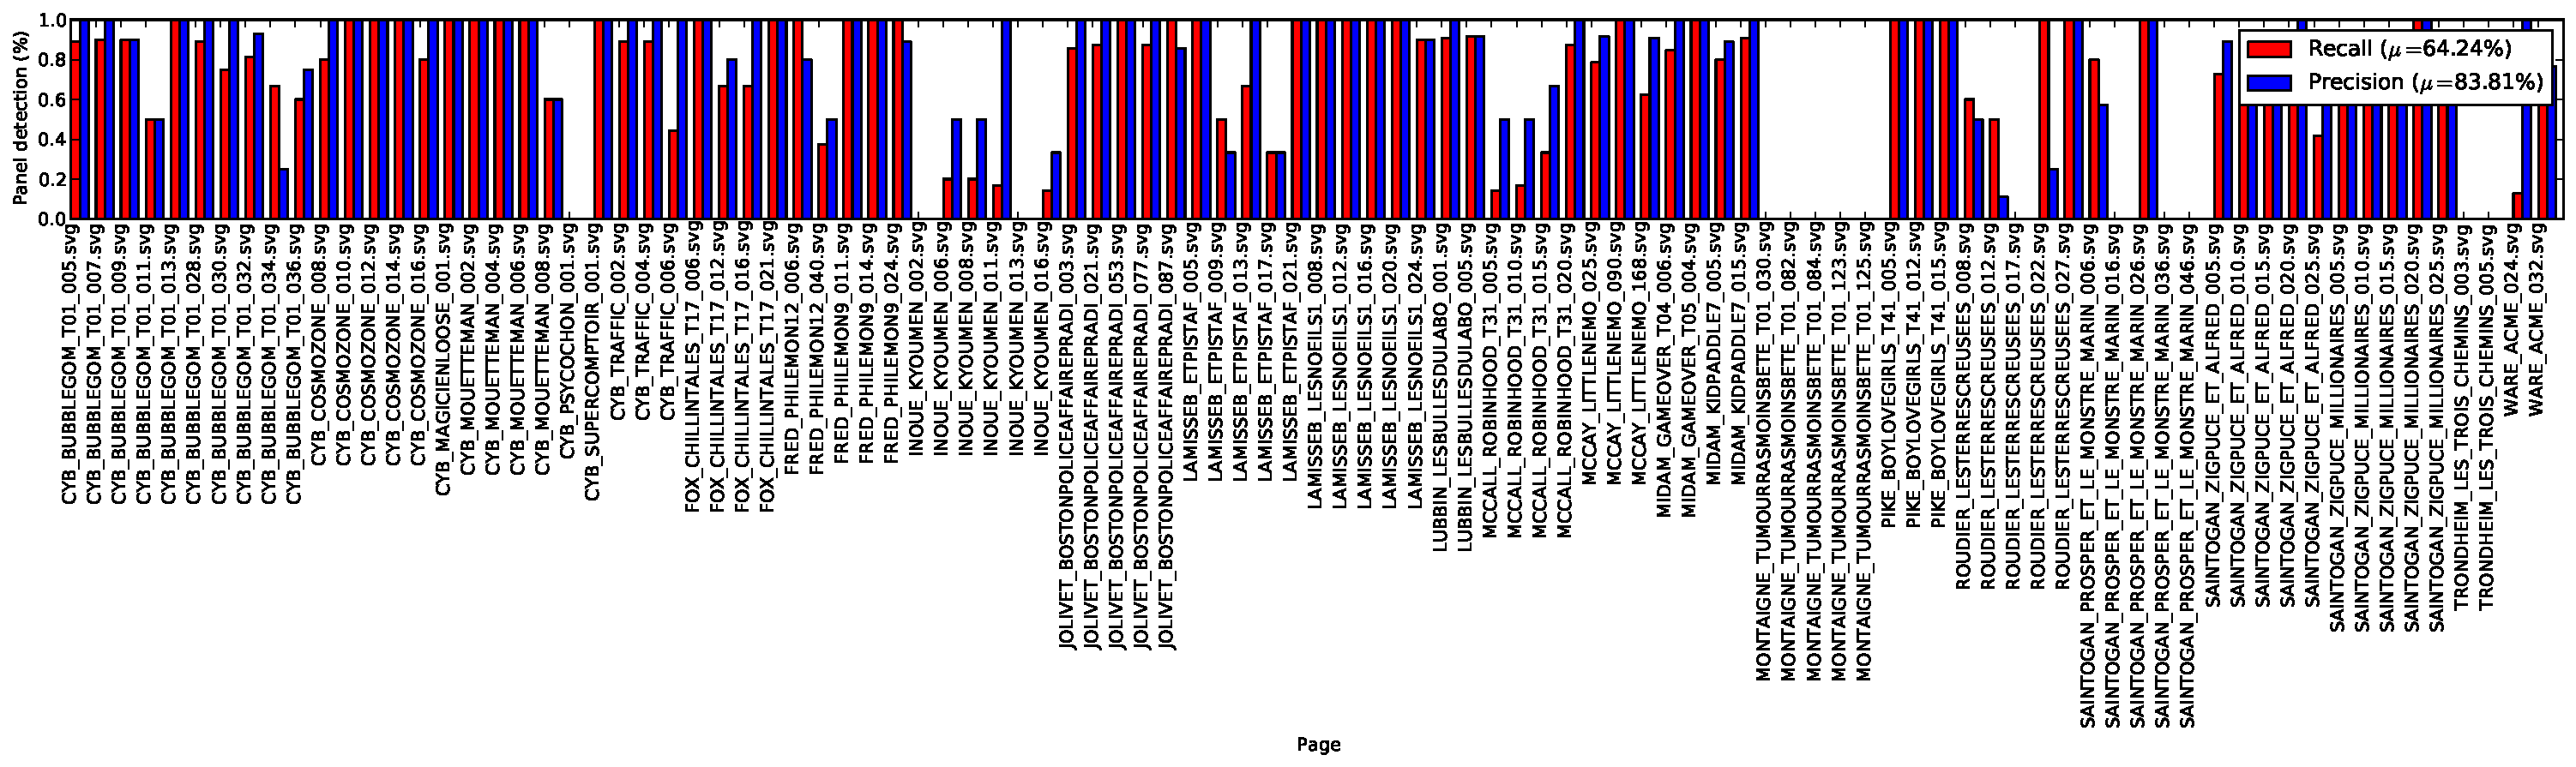
\includegraphics[trim= 0mm 108mm 0mm 0mm, clip, width=\textwidth]{2014-07-24_svg_Rigaud2012LNCS_Method_APanel_object.pdf}}
  %\hspace{1em}
  \\
  % \subfloat[Method A]{\label{fig:in:panel_outermost_contours}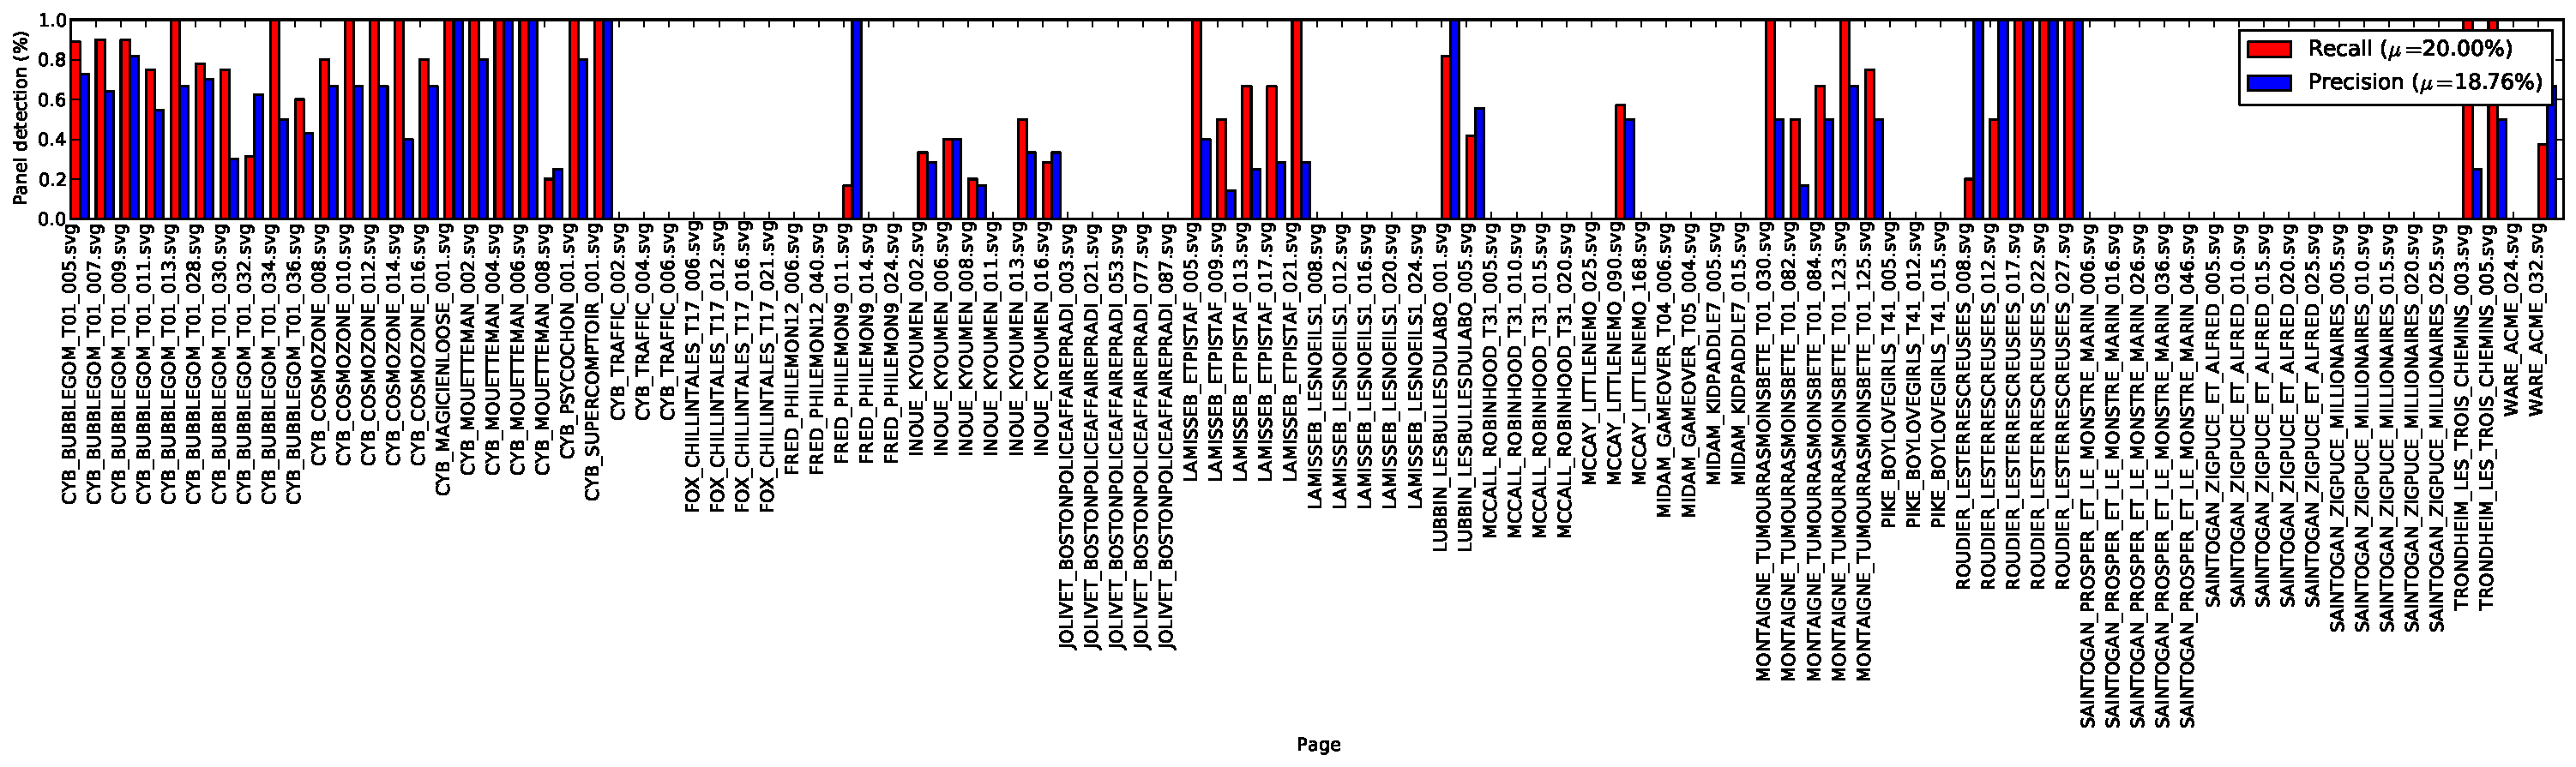
\includegraphics[trim= 0mm 0mm 0mm 0mm, clip, width=\textwidth,height=4cm\textwidth]{2014-07-20_svg_Arai2010_no_division_linePanel_object.pdf}}
  % \\
  \subfloat[Method I]{\label{fig:ex:panel_methodB_extraction_detail}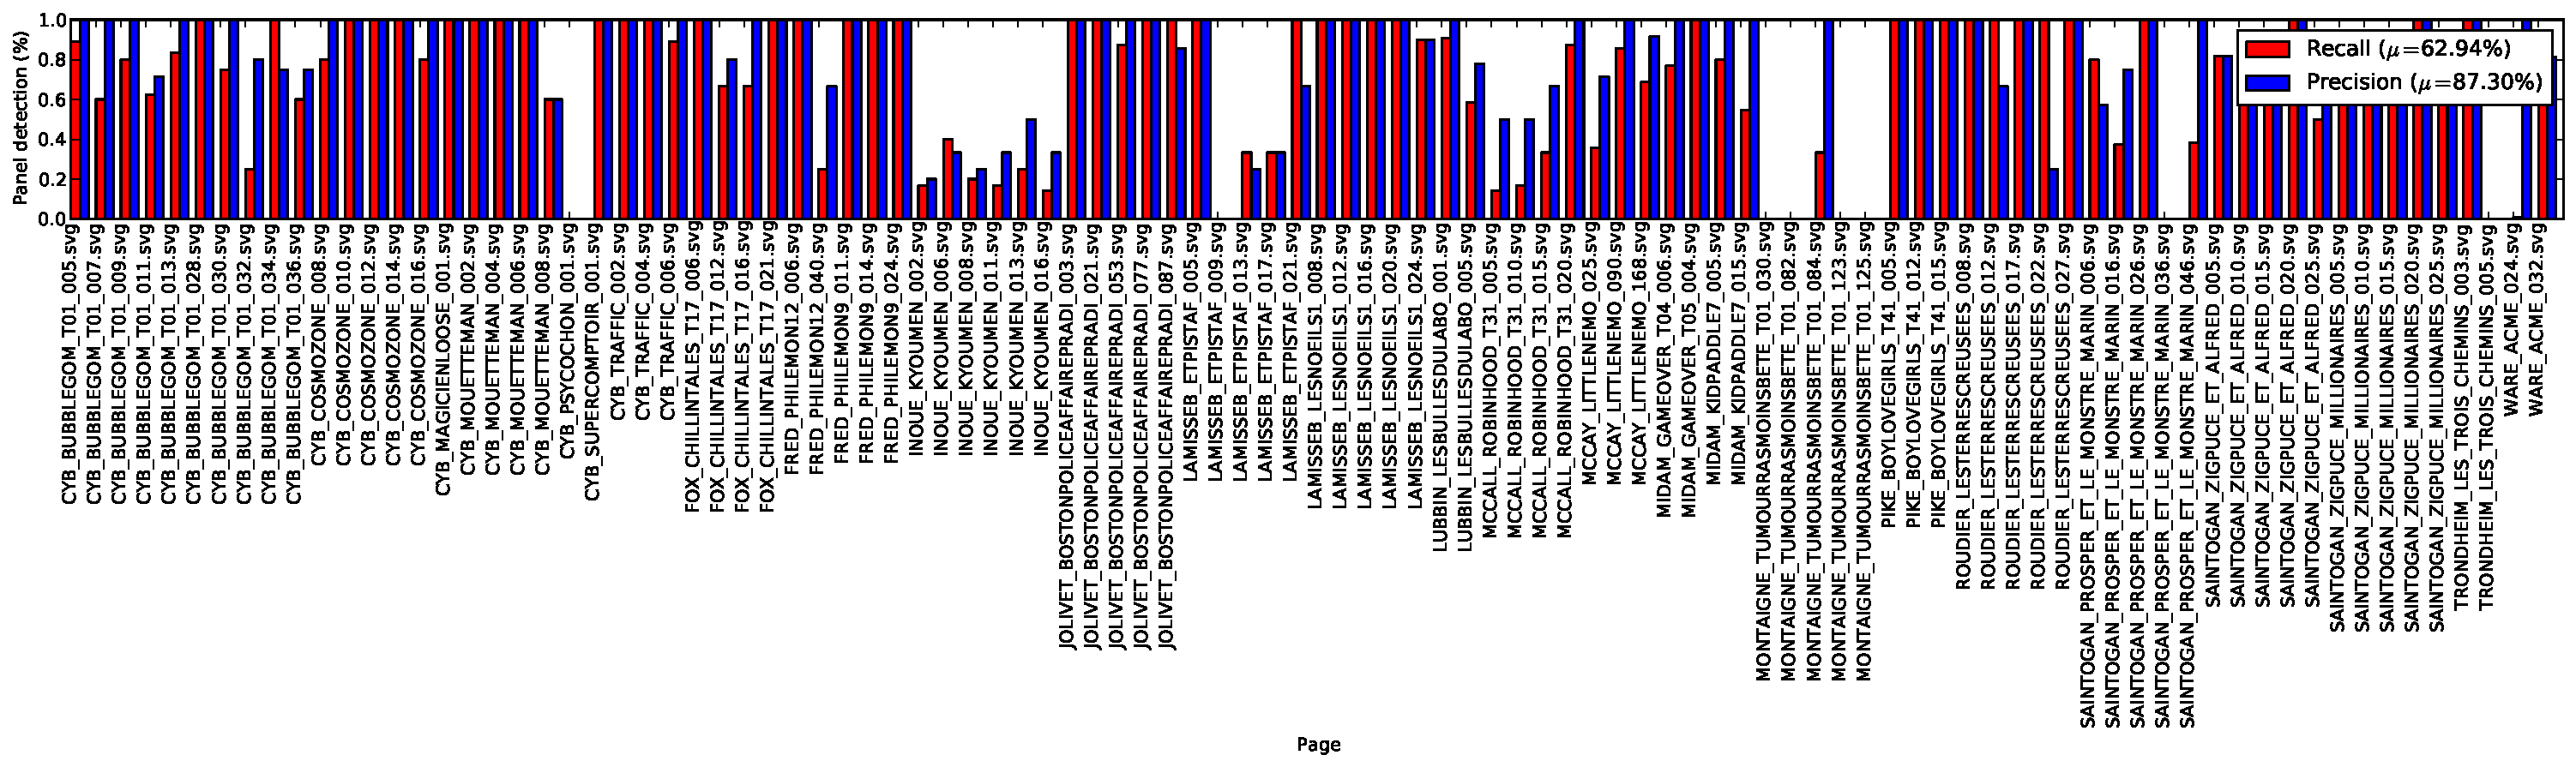
\includegraphics[trim= 0mm 108mm 0mm 0mm, clip, width=\textwidth]{2014-08-19_svg_Rigaud2014Outermost_Method_BPanel_object.pdf}}% \hspace{1em}
  \\
  % \subfloat[Method A]{\label{fig:in:panel_outermost_contours}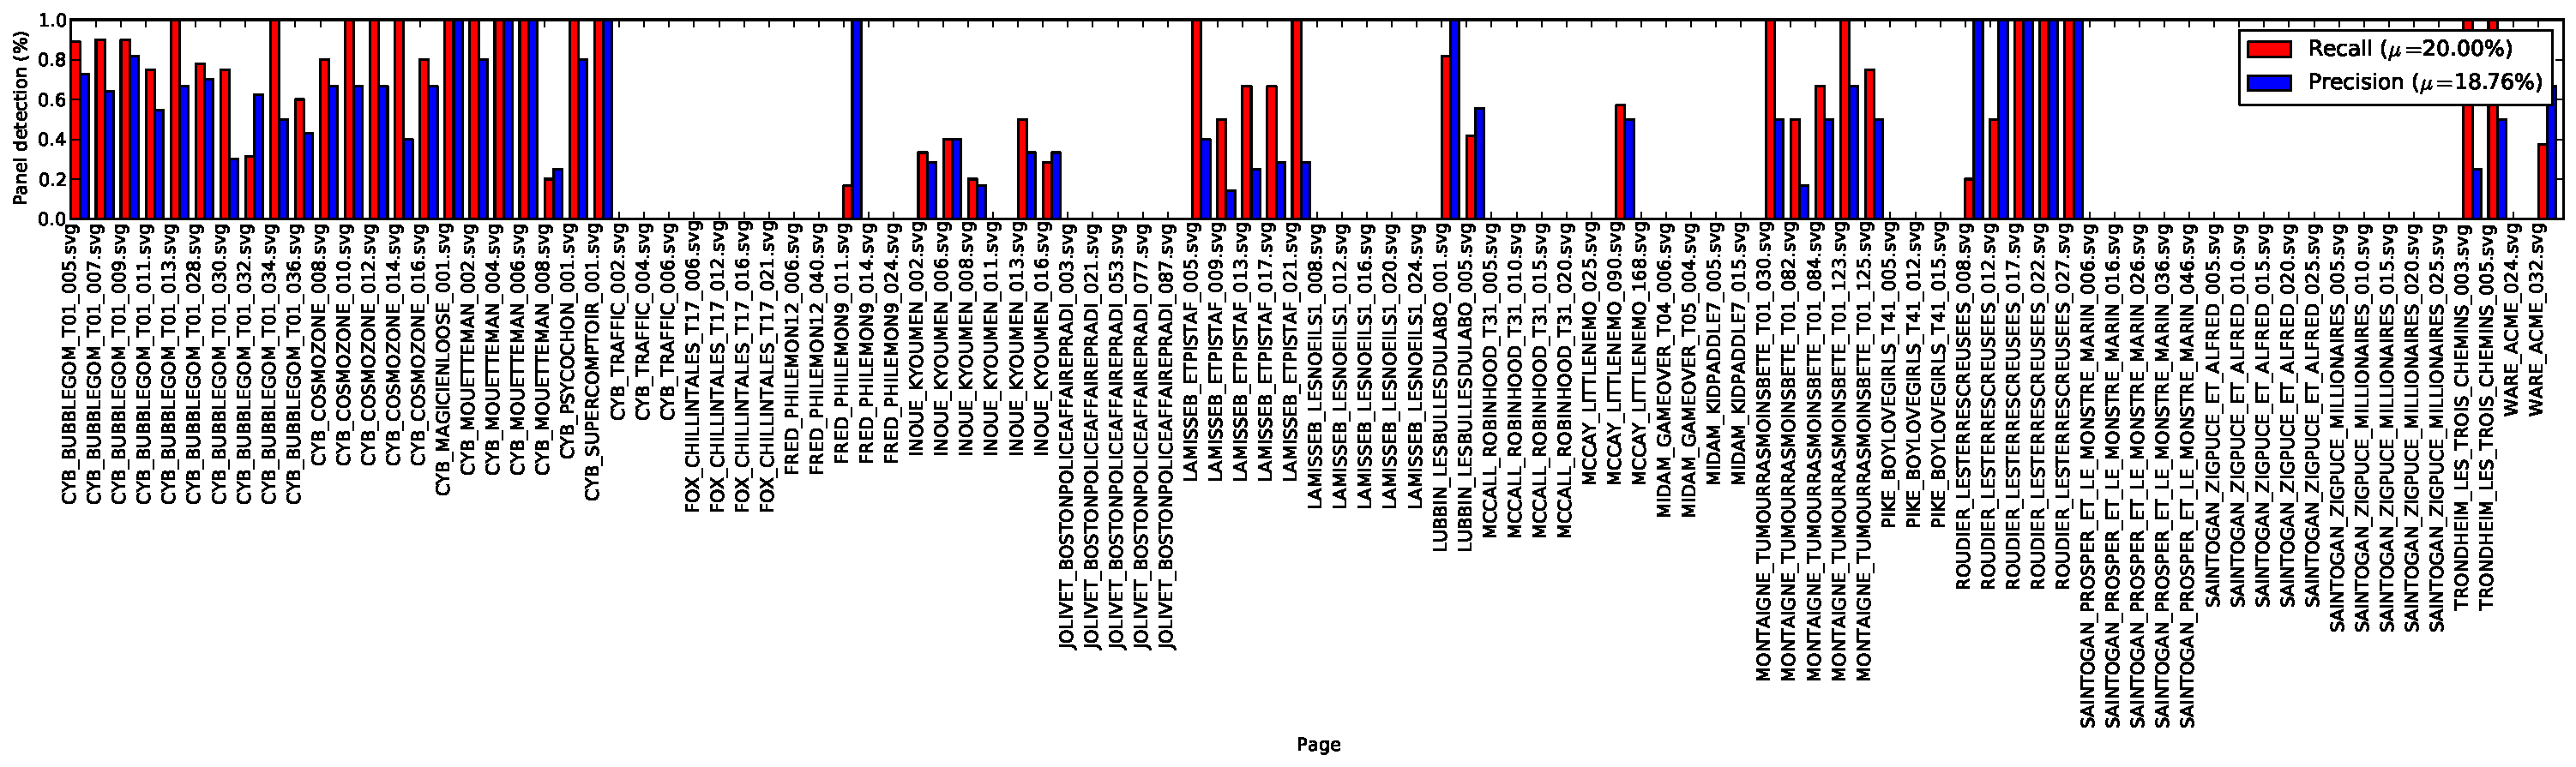
\includegraphics[trim= 0mm 0mm 0mm 0mm, clip, width=\textwidth,height=4cm\textwidth]{2014-07-20_svg_Arai2010_no_division_linePanel_object.pdf}}
  % \\
  \subfloat[Method K]{\label{fig:ex:panel_methodC_extraction_detail}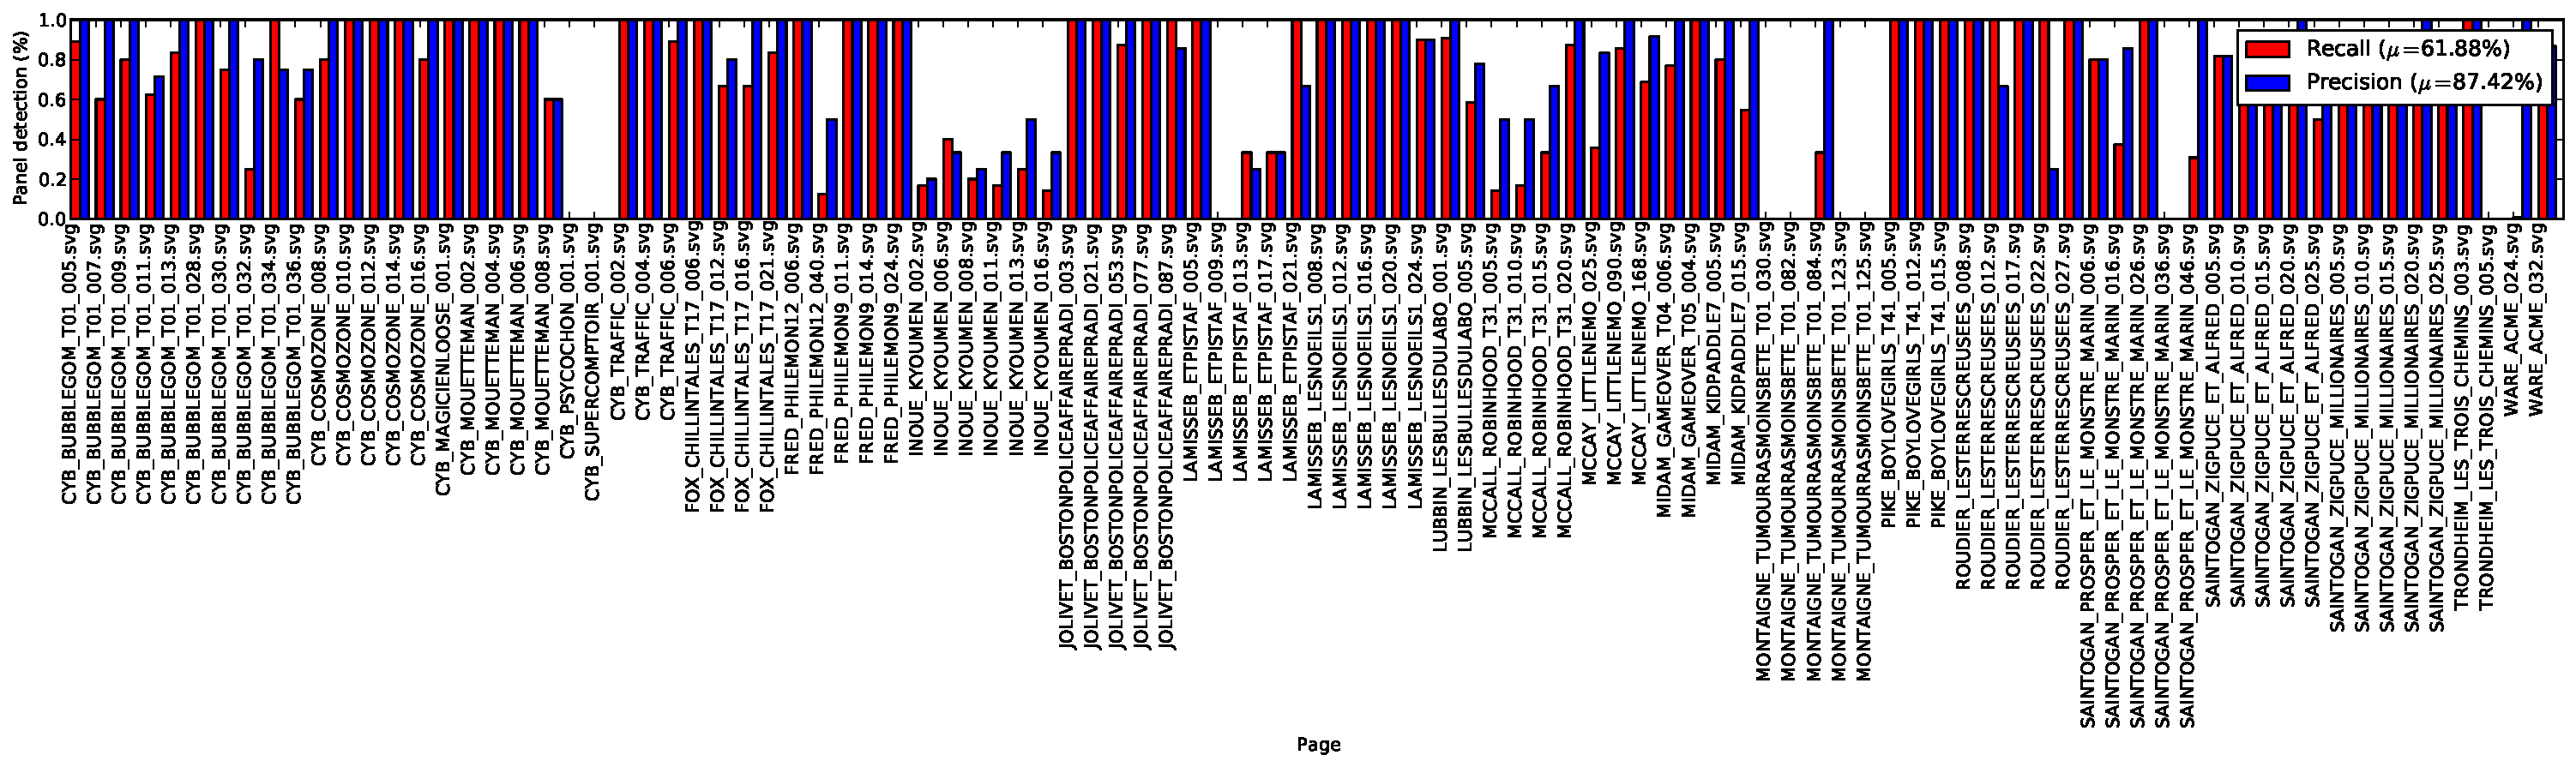
\includegraphics[trim= 0mm 0mm 0mm 0mm, clip, width=\textwidth]{2014-09-04_cleaned_validated_from_method_B_for_panel_text_balloon_and_method_A_for_character_Panel.pdf}}% \hspace{1em}
  % \\
  % \subfloat[Method C]{\label{fig:in:panel_big_contour_hull}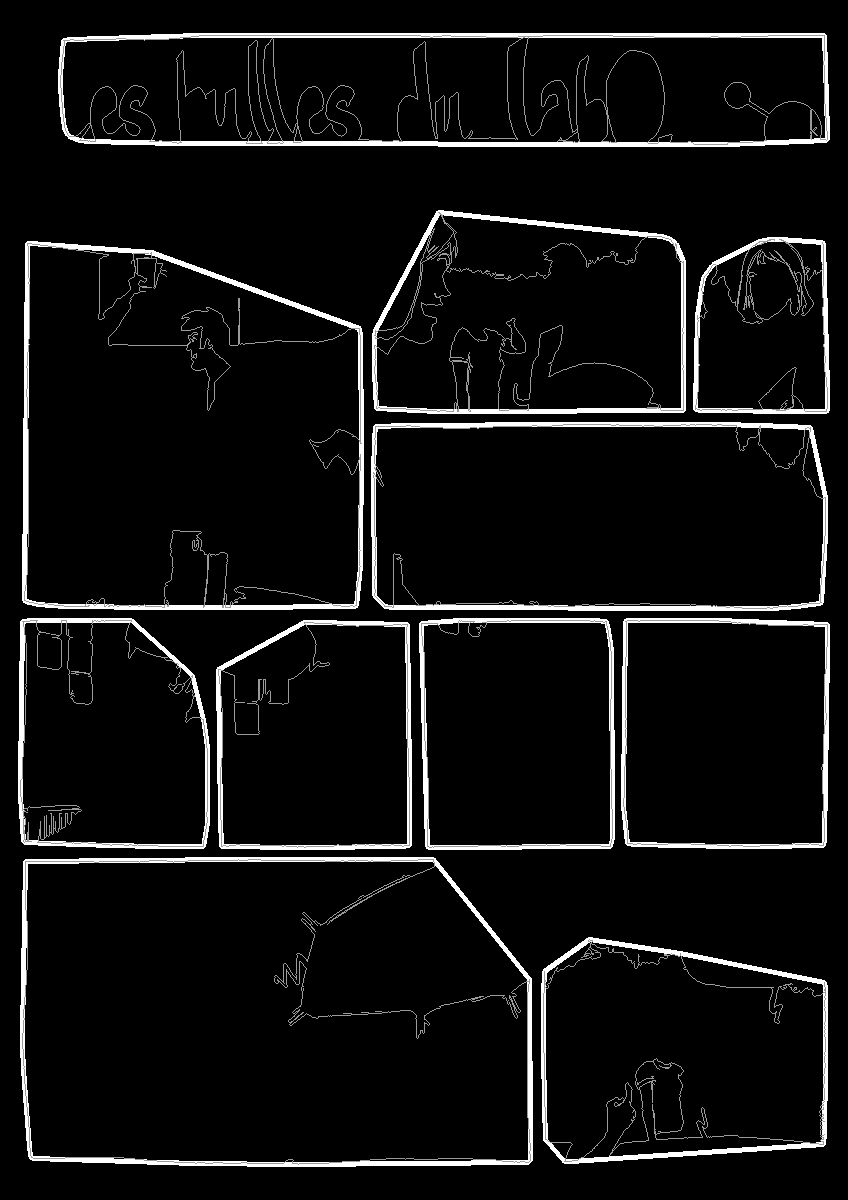
\includegraphics[trim= 0mm 0mm 0mm 0mm, clip, width=\textwidth,height=4cm]{panel_big_contour_hull.png}}
    \caption[Panel extraction score details for each image of the eBDtheque dataset]{Panel extraction score details for each image of the eBDtheque dataset (Appendix~\ref{app:dataset}).}
    \label{fig:ex:panel_detection_result_details}
\end{figure}
%%%%%%%%%%%%%%%%%%%%%%%%%%%%%%%%%%%%%%%%%%%%%%%%%%%


%-----------------------------------------------------------
\subsection{Comparison and analysis} % (fold)
\label{sub:result_analysis}

Table~\ref{tab:panel_extraction_comparision_results} compares the average results we obtained for the three proposed methods and two methods from the literature.
Note that some of the dataset images were digitized with a dark background surrounding the cover of the book.
We automatically remove this by cropping the image where a panel with an area greater than 90\% of the page area is detected.


    %%%%%%%%%%%%%%%%%%%%%%%%%%%%%%%%%%%%%%%%%%%%%%%%%%%
  \begin{table}[ht]
    \normalsize
%\renewcommand{\arraystretch}{1.2}

    \centering
    \caption[Panel extraction evaluation results]{Panel extraction evaluation results.}
    \begin{tabular}{|c|c|c|c|}
          % \hline
          %   & \multicolumn{2}{|c|}{Character 1}   & \multicolumn{2}{|c|}{Character 2}   \\
          \hline
          &  $R$ (\%)  & $P$ (\%)  & $F$ (\%)     \\
          \hline
          Arai~\cite{Arai11}   & 20.0       & 18.75    & 19.35    \\
          \hline
          Ho~\cite{Ho2012}   & 49.76       & 68.74    & 57.48    \\
          \hline
          Method S          & \textbf{64.24}       & 83.81   & 72.72     \\
          \hline
          Method I          & 62.94       & 87.30   & \bf{73.14}      \\
          \hline
          Method K          & 61.88       & \textbf{87.42}     & 72.46      \\
          \hline
        \end{tabular}
    \label{tab:panel_extraction_comparision_results}
  \end{table}%
    %%%%%%%%%%%%%%%%%%%%%%%%%%%%%%%%%%%%%%%%%%%%%%%%%%%

%TODO: re evaluate Arai's result from his method (still waiting for is email 2014-07-01)

The main drawback of the Arai's method is the binary segmentation with a fixed value that works best for comic book with a white background but it is not appropriate for digitization defaults and paper yellowing.
This method is only appropriate for webcomics with a perfectly white background clear separation between panels (Figure~\ref{fig:ex:panel_arai_extraction_detail}).

Ho's method is adaptive to background variation but considers as panel all the elements that are directly included (first topological level) in the page background.
This produce an over-segmentation by including some text which are inside the frame-less panels or inside implicit balloons.
When those out of panel elements are small, they prevent the connected panel separation process to work properly because the stopping criterion is based on element size.

The first method we proposed (Method S) extracts panel and text simultaneously and then other elements in a sequential manner.
It assumes that there are the distinguishable cluster of connected-component height in the image which is not always the case in this dataset.
Anyway, it still more powerful that the two method from the literature, mainly because of the more generic pre-processing steps.

The second proposed panel extraction method (Method I), based on connected-component clustering, is simple to implement, fast and efficient for comics with disconnected panels (separated by a white gutter).
% Figure~\ref{ap:panel_extraction} shows the details for each image tested, which were mainly comics with gutters.
% The proposed method is not appropriate for gutterless comics such as ``INOUE'' or strip without panel border such as ``MONTAIGNE'' or a extra frame around several panels (``SAINTOGAN\_PROSPER'').
This method is not appropriate for gutterless comics (e.b. some mangas) or strip without panel borders such as those with an extra frame around several panels.
Another weakness is when panels are connected by other elements, they may not be split as desired but will remain clustered as panel anyway.

Method K benefits form the domain knowledge to filter out irrelevant panel candidates from the independent extraction approach (Method I).
Nevertheless, the validation by the expert system was not significant here because the low level processing had already reached the limits of the model (Section~\ref{sub:kn:comics_domain}).

% This experiment was performed in \modif{??} seconds for the whole dataset using one CPU at 2.5GHz (\modif{??}s per panel on average).

% subsection result_analysis (end)


% subsection sequential_panel_extraction_evaluation (end)


\section{Text extraction evaluation} % (fold)
\label{sub:ex:text_extraction_recognition_evaluation}

In this section we evaluated our three propositions for text extraction and compare them to a methods from the literature.
We selected Arai's method as it is the most advanced method that have been applied to comic book images.
All the evaluations of text localisation were performed on the 4691 text lines of the eBDtheque dataset~\cite{Guerin2013} at object bounding box level (Section~\ref{sub:ex:object_localisation_metric}).
Text recognition evaluations have been performed on the same dataset but using the accuracy metric presented in Section~\ref{sub:ex:text_recognition_metric}.

% \subsection{Experimental settings} % (fold)
% % \label{sub:experimental_settings}

% TODO

\subsection{Arai's method} % (fold)
We implemented Arai's method~\cite{Arai11} which is a sequential approach that requires panel and balloon extraction as input, as presented in Section~\ref{sub:ex:panel_extraction_arai} and~\ref{sub:ex:balloon_extraction_arai} respectively.
This method was developed for grey-scale Japanese mangas and is divided in five steps: pre-processing, blob extraction, feature extraction, text blob selection and text blob extraction.
Pre-processing consists in an adaptive bi-level segmentation at 30\% (chosen empirically) above the average pixel value and mathematical morphology to group potential text letters into block (similar to the Run Length Smoothing Algorithm).
Note that the threshold selection method can exceed the maximal pixel value and then produce an empty segmentation.
The size of the kernel was not specified in the original paper, we used $3*5$ pixels.
Blob extraction is performed by imposing a minimal size of the blob relatively to the size of the balloon in which they are included ($Balloon.width / 20$ and $Balloon.hight / 40$).
The extracted features are the \emph{average text blob width} and the horizontal coordinate of its centroid.
These features are used to classify text / non-text blobs according to two rules based on blob inter-distances and alignments.
Text blob are then extracted from the original image and directly sent to an OCR system (Figure~\ref{fig:ex:balloon_extraction_arai}).

%%%%%%%%%%%%%%%%%%%%%%%%%%%%%%%%%%%%%%%%%%%%%%%%%%%%%%
\begin{figure}[h]
 \centering
 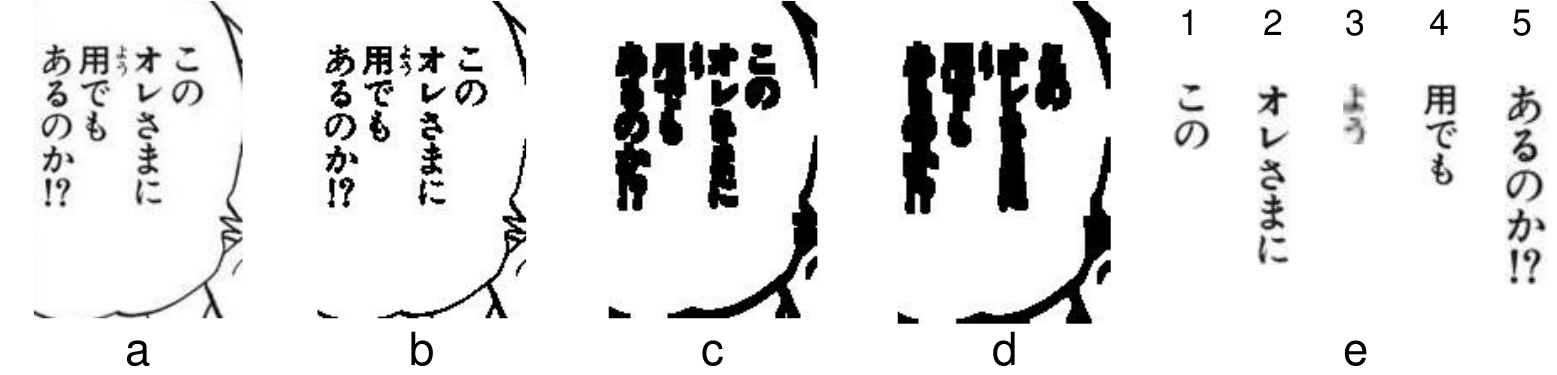
\includegraphics[width=0.9\textwidth]{balloon_extraction_arai.png}
 \caption[Sample of text extraction process of Arai's method]{Sample of text extraction process. (a) Original balloon text image; (b) Threshold; (c) Morphology-Erosion filter; (d) Morphology-Opening filter; (e) Extracted blob from original image. Image from the original paper~\cite{Arai11}.
 }
 \label{fig:ex:balloon_extraction_arai}
\end{figure}
%%%%%%%%%%%%%%%%%%%%%%%%%%%%%%%%%%%%%%%%%%%%%%%%%%%%%%

This approach was only developed for vertical text block extraction but we adapt it to also handle horizontal text.
Its adaptation to horizontal text consists in switching width and height related parameters in the pre-processing and feature extraction steps.
Also, the kernel used for mathematical morphology is rotated of 90$^{\circ}$.

The score of this method was in average for recall and precision of 2.81\% and 1.63\% (Figure~\ref{fig:ex:text_arai_extraction_detail}).

\subsection{Sequential approach} % (fold)
% \label{sub:method_1}
The method proposed in Section~\ref{sec:se:panel_and_text} does not require any particular parameter, only the number of clusters has to be fixed $k=3$ for the reason explained in the presentation of the method (Section~\ref{sec:se:panel_and_text}).
Note that the method is designed to simultaneously extract panel regions which does not interfere with text.
The score of this method  was in average for recall and precision of 54.68\% and 56.92\% (Figure~\ref{fig:ex:text_methodA_extraction_detail}).

% %%%%%%%%%%%%%%%%%%%%%%%%%%%%%%%%%%%%%%%%%%%%%%%%%%%%%%
% \begin{figure}[h]
%  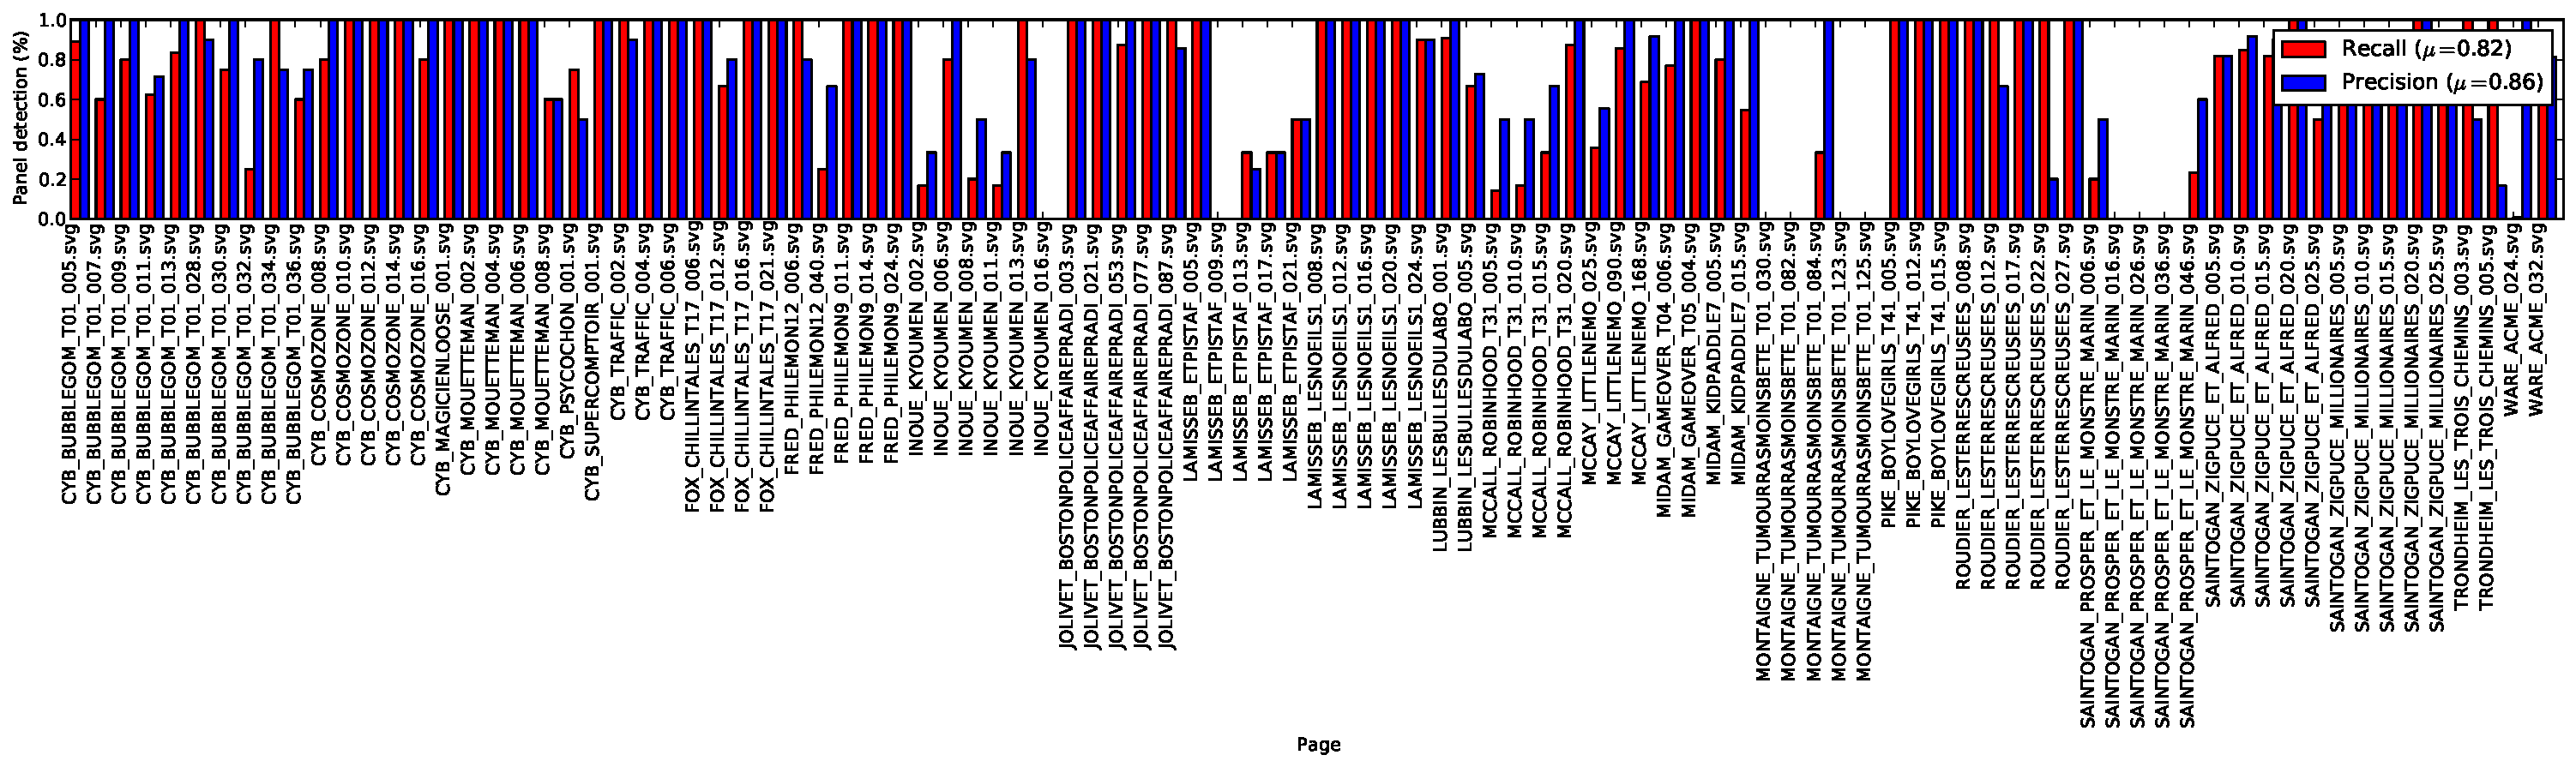
\includegraphics[width=\textwidth,height=4cm]{Panel_object_proposed.pdf}
%  \caption{Text extraction score details using Method A for each image of the eBDtheque dataset \modif{TODO: update}.
%  }
%  \label{fig:ex:text_methodA_extraction_detail}
% \end{figure}
% %%%%%%%%%%%%%%%%%%%%%%%%%%%%%%%%%%%%%%%%%%%%%%%%%%%%%%


% subsection method_1 (end)
\subsection{Independent approach} % (fold)
\label{sub:ex:text_extraction_evaluation_method_b}

The method presented in Section~\ref{sec:in:text_localisation_and_recognition} consists in a bi-level segmentation, text/graphic separation, text line generation and finally text line recognition.
A comparison between two threshold selection methods and two colour-to-grey image conversion are shown in Table~\ref{fig:ex:text_extraction_methodB_segmentation}.

%%%%%%%%%%%%%%%%%%%%%%%%%%%%%%%%%%%%%%%%%%%%%%%%%%%

  \begin{table}[ht]
    % \normalsize
    \centering
    \caption[F-measure results for fixed and adaptive threshold selection method corresponding to combined and separated colour to grey conversion methods]{F-measure results for fixed ($th=250$) and adaptive threshold selection method corresponding to combined (RGB to grey) and separated (Luminance layer) colour to grey conversion methods.}
    \begin{tabular}{|c|c|c|}
      \hline
       & Fixed & Otsu \\ 
      \hline
      RGB to grey & 11.74 & \textbf{51.35}  \\ 
      \hline
      Luminance layer & 11.66 & 51.31 \\ 
      \hline
    \end{tabular}
    \label{fig:ex:text_extraction_methodB_segmentation}
  \end{table}%

  % \begin{figure}[!ht]%trim=l b r t  width=0.5\textwidth,
  % \begin{center}
  %   \begin{tabular}{|c|c|c|}
  %     \hline
  %      & Fixed & Otsu \\ 
  %     \hline
  %     RGB to grey & \modif{??} & \modif{??}  \\ 
  %     \hline
  %     Luminance layer & \modif{??} & \modif{??} \\ 
  %     \hline
  %   \end{tabular}
  % \caption[Results for fixed and adaptive threshold selection method corresponding to combined and separated colour to grey conversion methods]{Results for fixed ($th=250$) and adaptive threshold selection method corresponding to combined (RGB to grey) and separated (Luminance layer) colour to grey conversion methods.}
  % \label{fig:ex:text_extraction_methodB_segmentation}
  % \end{center}
  % \end{figure}  
  %%%%%%%%%%%%%%%%%%%%%%%%%%%%%%%%%%%%%%%%%%%%%%%%%%%

Text and graphics separation is performed using the Mahalanobis' distance which is related to the number of standard deviations.
A validation on the eBDtheque dataset shown that the best Mahalanobis' distance is $d_m=2$.
% The similarity offset $a$ and the overlapping percentage $b$ have been also validated over the eBDtheque dataset and their best values are $a=$\modif{???} and $b=$\modif{???} respectively.
Text line recognition is used as last filtering operation to validate the presence of text inside the candidate regions, its average benefit is shown in Table~\ref{tab:text_results}.
The score of this method was in average for recall and precision of 64.14\% and 70.28\% (Figure~\ref{fig:ex:text_methodB_extraction_detail}).

%The detailed results using the OCR system are given Figure~\ref{fig:ex:text_methodB_extraction_detail}.


%%%%%%%%%%%%%%%%%%%%%%%%%%%%%%%%%%%%%%%%%%%%%%%%%%%%%%
% \begin{figure}[h]
%  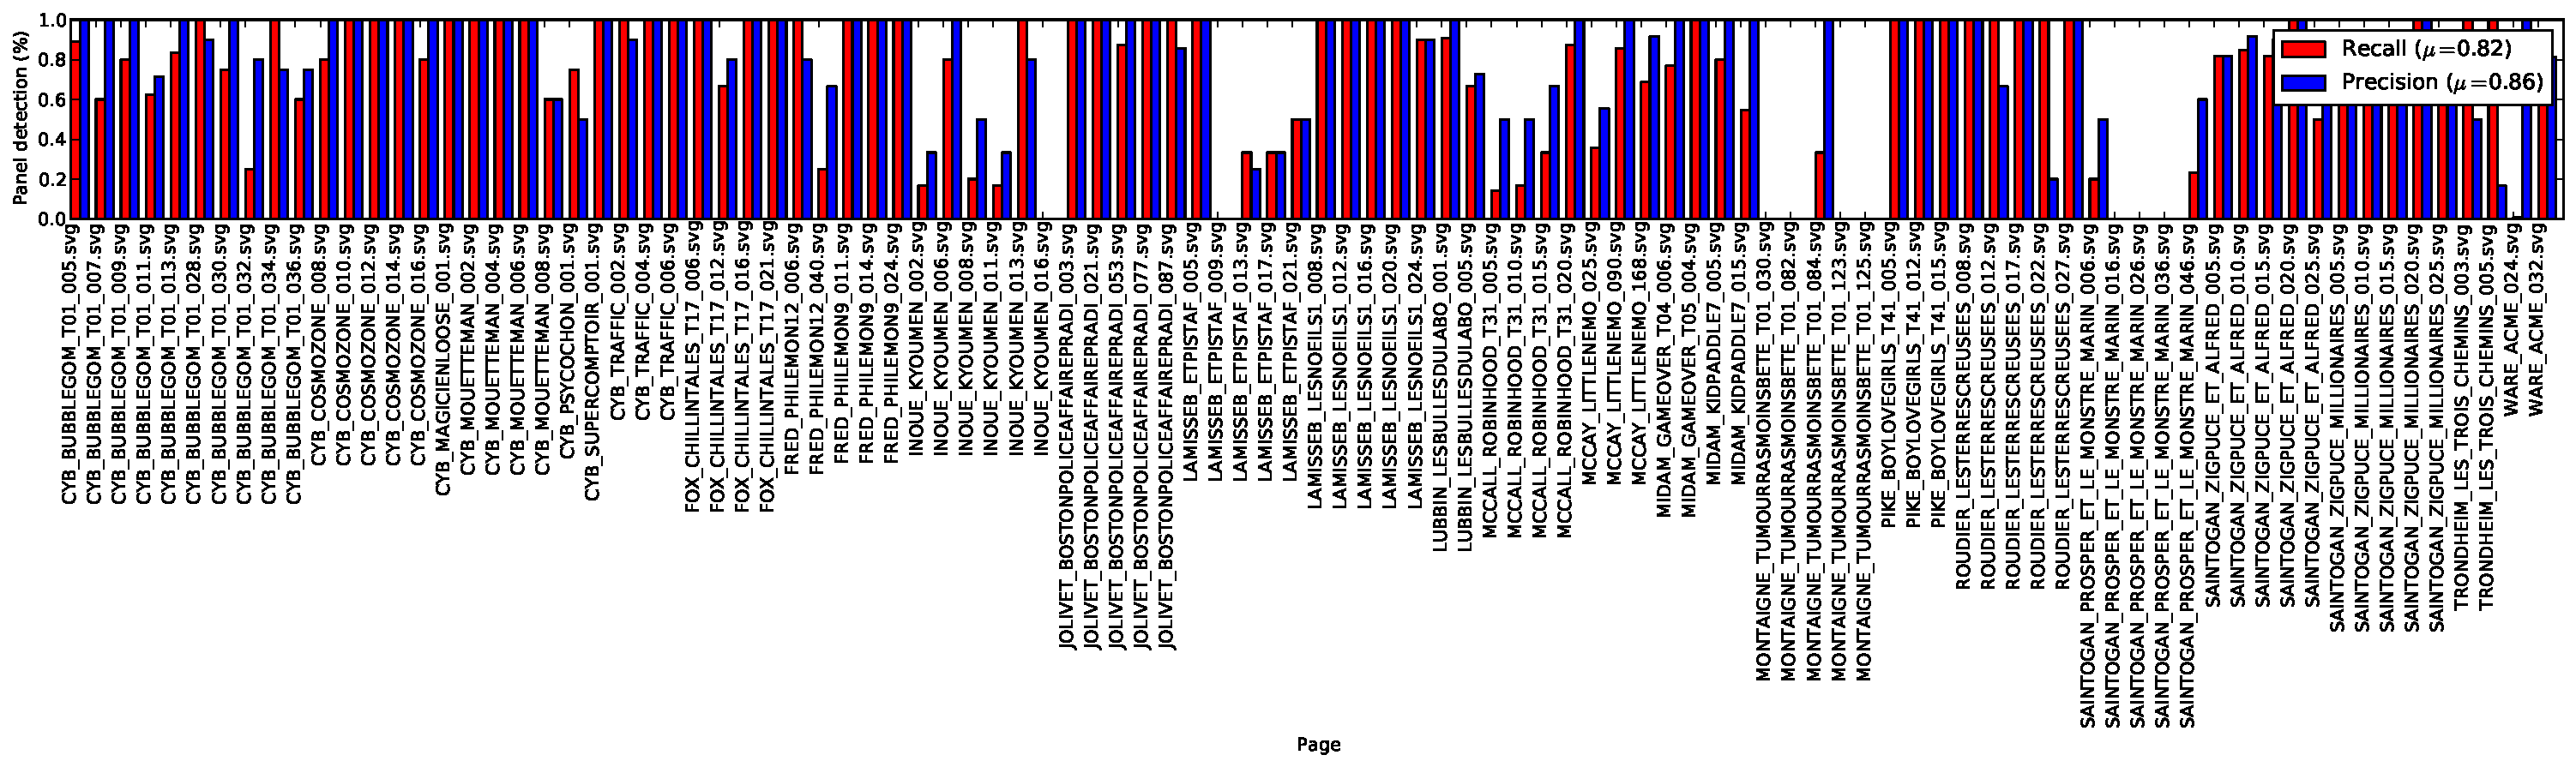
\includegraphics[width=\textwidth,height=4cm]{Panel_object_proposed.pdf}
%  \caption{Text extraction score details using Method B and the best bi-level combination method (Otsu + Luminance) for each image of the eBDtheque dataset \modif{TODO: update}.
%  }
%  \label{fig:ex:text_methodB_extraction_detail}
% \end{figure}
%%%%%%%%%%%%%%%%%%%%%%%%%%%%%%%%%%%%%%%%%%%%%%%%%%%%%%


% subsection method_b (end)

\subsection{Knowledge-driven approach} % (fold)
% \label{sub:method_c}

The knowledge-driven method can be used as a post processing of the text extraction.
It validates or rejects text candidates using the proposed model (Section~\ref{sec:kn:processing_sequence}).
In the model, the only rule concerning text location is that they should be contained in a panel.
Considering the best method for panel and text extraction method from Tables~\ref{tab:panel_extraction_comparision_results} and~\ref{tab:text_results} respectively, the score of this method was in average for recall and precision of 39.99\% and 64.88\% (Figure~\ref{fig:ex:text_methodC_extraction_detail}).

%%%%%%%%%%%%%%%%%%%%%%%%%%%%%%%%%%%%%%%%%%%%%%%%%%%%%%
% \begin{figure}[h]
%  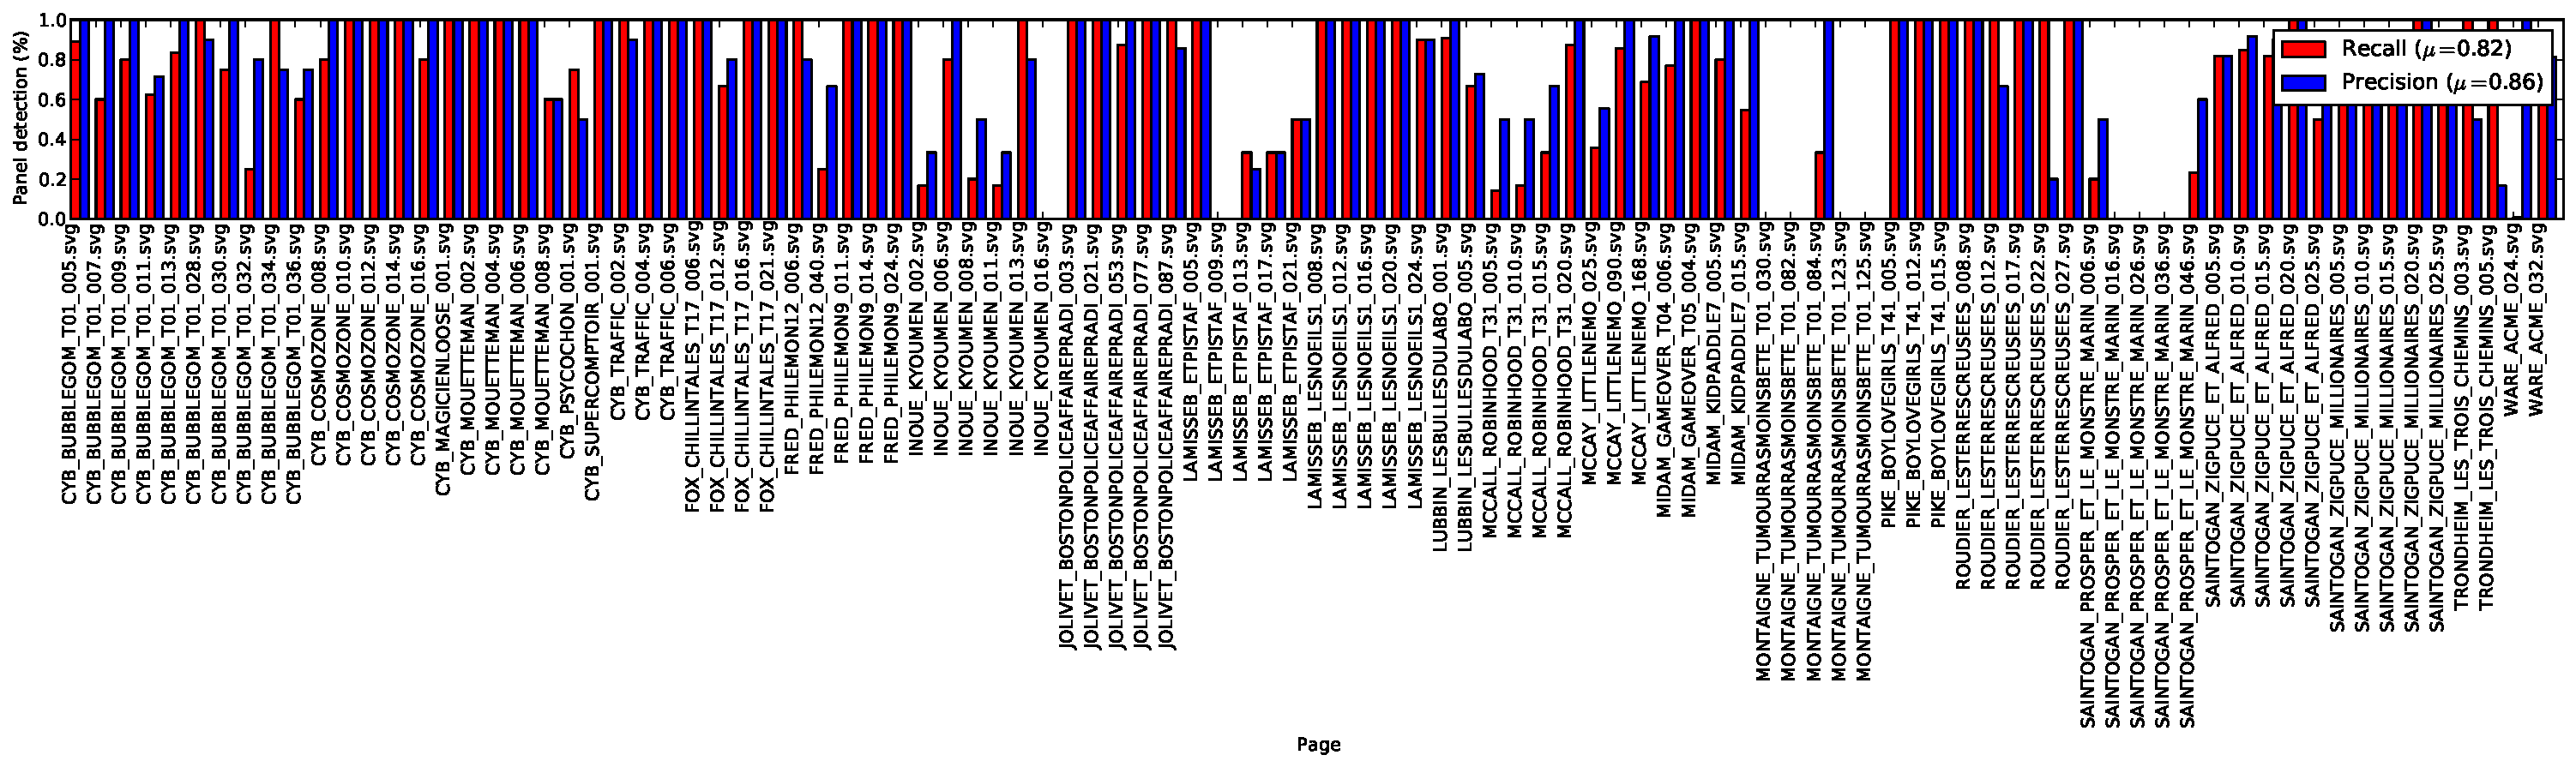
\includegraphics[width=\textwidth,height=4cm]{Panel_object_proposed.pdf}
%  \caption{Text extraction score details using Method C for each image of the eBDtheque dataset \modif{TODO: update}.
%  }
%  \label{fig:ex:text_methodC_extraction_detail}
% \end{figure}
%%%%%%%%%%%%%%%%%%%%%%%%%%%%%%%%%%%%%%%%%%%%%%%%%%%%%%

% subsection method_c (end)

% subsection experimental_settings (end)




\subsection{Comparison and analysis} % (fold)
\label{sub:results_analysis}

Table~\ref{tab:text_results} summarise the recall, precision and f-measure of the experimented methods.

    %%%%%%%%%%%%%%%%%%%%%%%%%%%%%%%%%%%%%%%%%%%%%%%%%%%
  \begin{table}[ht]
    \normalsize
    \centering
    \caption{Text localisation results.}
    \begin{tabular}{|c|c|c|c|}
          % \hline
          %   & \multicolumn{2}{|c|}{Character 1}   & \multicolumn{2}{|c|}{Character 2}   \\
          \hline
          &  $R$ (\%)  & $P$ (\%)  & $F$ (\%)  \\
          % \hline
          % Before validation   & ?   & ?           \\
          \hline
          % Tanaka?\\ Chinese ICDAR? Stroke-based? Lluis?  & \modif{??}   & \modif{??}    & \modif{??}       \\
          % \hline
          Arai~\cite{Arai11}  & 2.81    & 1.63      & 2.07       \\
          \hline
          Method S            & 54.91   & 57.15     & 56.01       \\
          \hline
          Method I (without OCR)  & \textbf{67.21}   & 41.54    & 51.35       \\
          \hline
          Method I (with OCR)  & 64.14   & \textbf{70.28}    & \textbf{67.07}       \\
          \hline
          Method K  & 39.99   & 64.88    & 49.48       \\
          \hline
          % Proposed (\cite{Rigaud2013VISAPP}+OCR)  & 60.13   & 42.43   & 49.75        \\
          % \hline
          % Proposed + validation   & 44.54     & 65.05     & 52.88      \\
          % \hline
          %Proposed (\cite{Rigaud2013VISAPP}+OCR+$ST$ only)  & ?   & ?   & ?        \\
          % \hline
          % Proposed (OCR transcription)  & ?   & ?           \\
          % \hline
        \end{tabular}
    \label{tab:text_results}
  \end{table}%
    %%%%%%%%%%%%%%%%%%%%%%%%%%%%%%%%%%%%%%%%%%%%%%%%%%%

% In our previous work~\cite{Rigaud2013VISAPP} text extraction was evaluated on a subset of 20 pages of the eBDtheque dataset~\cite{Guerin2013}.
% Here we applied it to the whole dataset.
% We used our previous method as a baseline to show an improvement in the precision of 20\% when using an OCR-based filter, without a significant loss in recall.
% The validation by the expert system improved the precision as expected but also resulted in a drop in recall.
% The drop in recall can be explained by the fact that the text extractor is also able to detect texts which are not in the speech balloons but the model considers them as noise.
% in recall that could probably be filled for specific writing style by training the OCR on a specific font. %, when using an OCR system to filter out non text regions.

    %%%%%%%%%%%%%%%%%%%%%%%%%%%%%%%%%%%%%%%%%%%%%%%%%%%
  % \begin{table}[ht]
  %   \normalsize
  %   \centering
  %   \caption{Text localisation results.}
  %   \begin{tabular}{|c|c|c|c|}
  %         % \hline
  %         %   & \multicolumn{2}{|c|}{Character 1}   & \multicolumn{2}{|c|}{Character 2}   \\
  %         \hline
  %         &  $R$ (\%)  & $P$ (\%)  & $F$ (\%)  \\
  %         % \hline
  %         % Before validation   & ?   & ?           \\
  %         \hline
  %         Rigaud~\cite{Rigaud2013VISAPP}  & 61.00   & 19.66    & 29.75       \\
  %         \hline
  %         Proposed (\cite{Rigaud2013VISAPP}+OCR)  & 60.13   & 42.43   & 49.75        \\
  %         \hline
  %         Proposed + validation   & 44.54     & 65.05     & 52.88      \\
  %         % \hline
  %         %Proposed (\cite{Rigaud2013VISAPP}+OCR+$ST$ only)  & ?   & ?   & ?        \\
  %         % \hline
  %         % Proposed (OCR transcription)  & ?   & ?           \\
  %         \hline
  %       \end{tabular}
  %   \label{tab:text_results}
  % \end{table}%
    %%%%%%%%%%%%%%%%%%%%%%%%%%%%%%%%%%%%%%%%%%%%%%%%%%%

Arai's method is a sequential approach that requires panel and balloon regions as input.
As shown in Table~\ref{tab:ex:balloon_localisation_comparison_results}, balloon extraction is very low using this approach thus, it narrows down the text extraction in turn (Table~\ref{tab:text_results}).
Moreover, this text extraction method uses several thresholds which reduces its fields of application.


% In our previous work~\cite{Rigaud2013VISAPP} text extraction was evaluated on a subset of 20 pages of the eBDtheque dataset~\cite{Guerin2013}.
% Here we applied it to the whole dataset.
Method S improves by far the recall thanks to its genericity, moreover, even if the panel extraction is performed at the same time, it does not bias the text extraction because text areas are extracted from the whole page and not from panel regions.
Method I is slightly better using RGB to grey image conversion than the luminance layer only (Table~\ref{fig:ex:text_extraction_methodB_segmentation}).
It outperforms Method S in recall only when not using the last OCR filtering step and both recall and precision when using the OCR.
The difference for Method I when using or not the OCR system is about an increase of 26.74\% of precision and a loss 3.07\% of recall.
The validation by the expert system in Method K improved the precision as expected but also resulted in a drop in recall.
The drop of Method K can be explained by the fact that the text extractor is also able to detect texts which are not in the speech balloons but the model considers them as noise (rejected).
All the methods still encounter difficulties with certain types of text that can be found in the comics (e.g. illustrative text, graphic sounds) due to strong deformation or colour variations.


%%%%%%%%%%%%%%%%%%%%%%%%%%%%%%%%%%%%%%%%%%%%%%%%%%%
\begin{figure}[!ht] %trim=l b r t  width=0.5\textwidth, 
  \centering
  \subfloat[Arai's method]{\label{fig:ex:text_arai_extraction_detail}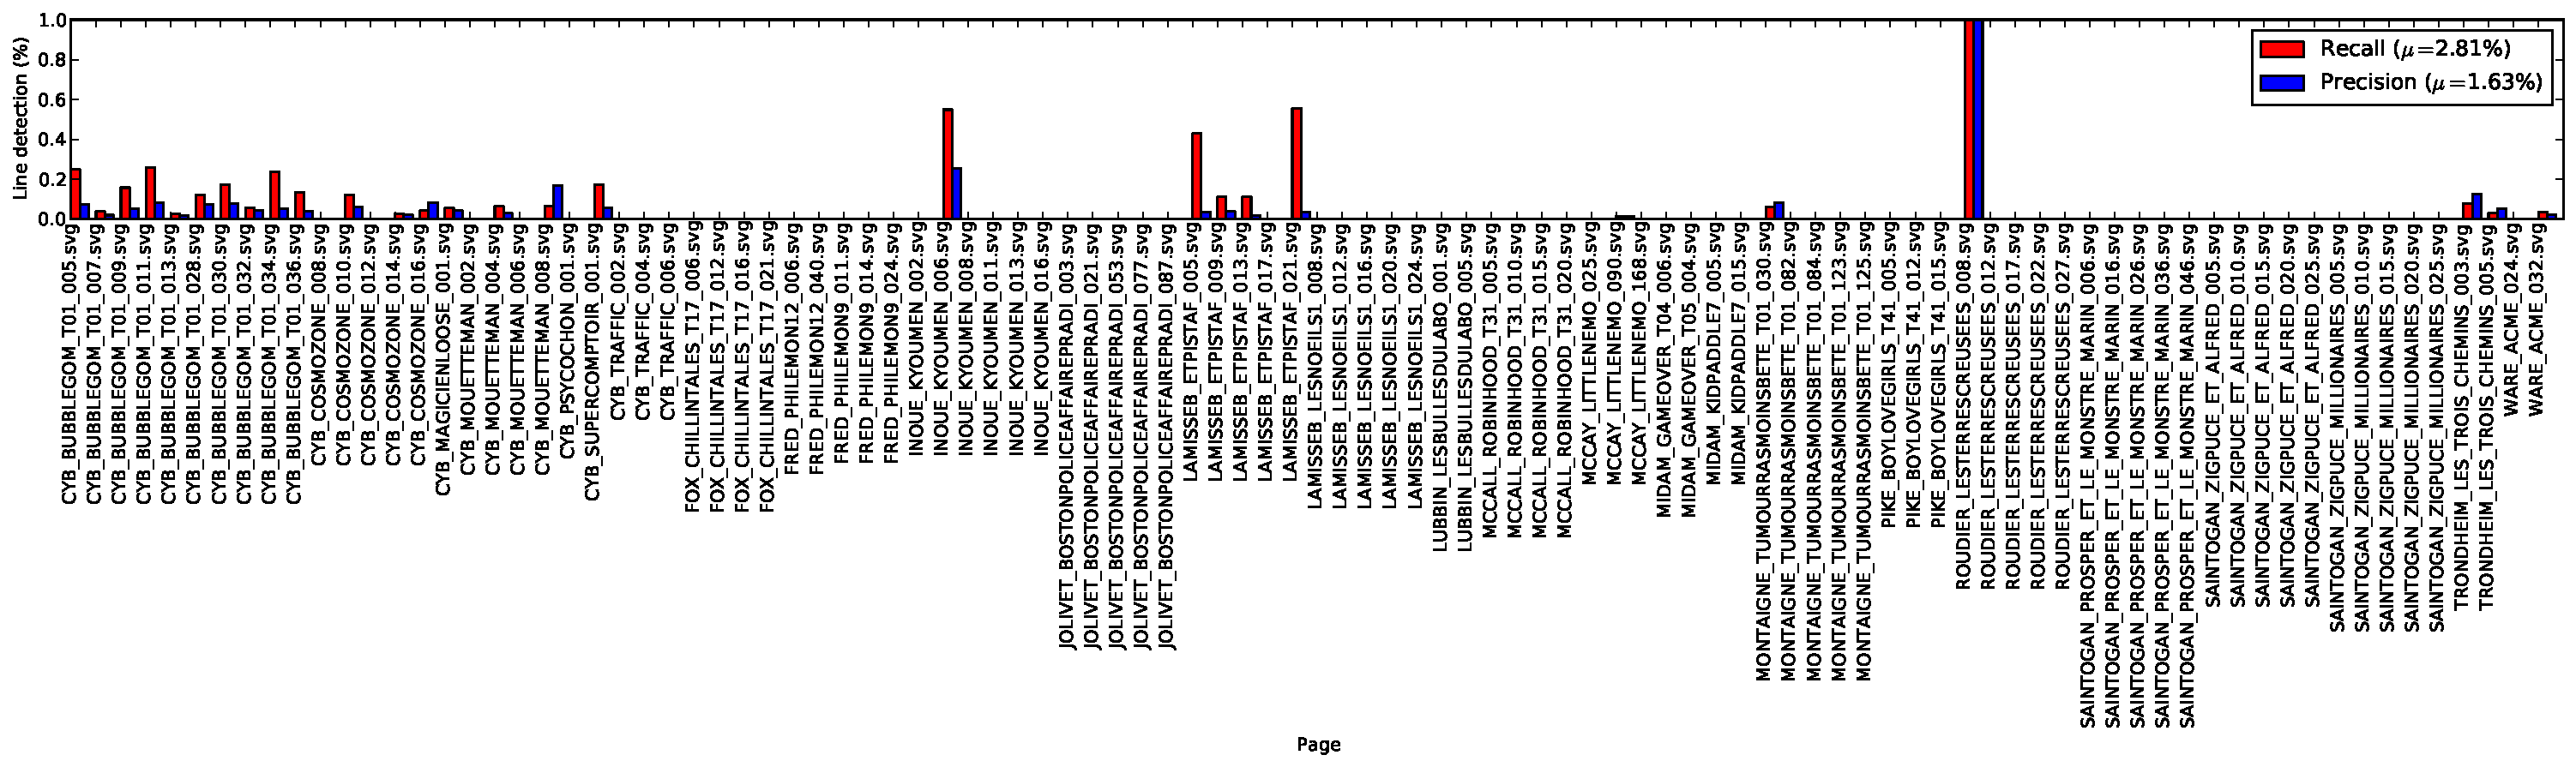
\includegraphics[trim= 0mm 108mm 0mm 0mm, clip, width=\textwidth]{2014-07-26_svg_Arai2011IJIPLine_object.pdf}}
  \\
  % \subfloat[Ho's method]{\label{fig:ex:panel_ho_extraction_detail}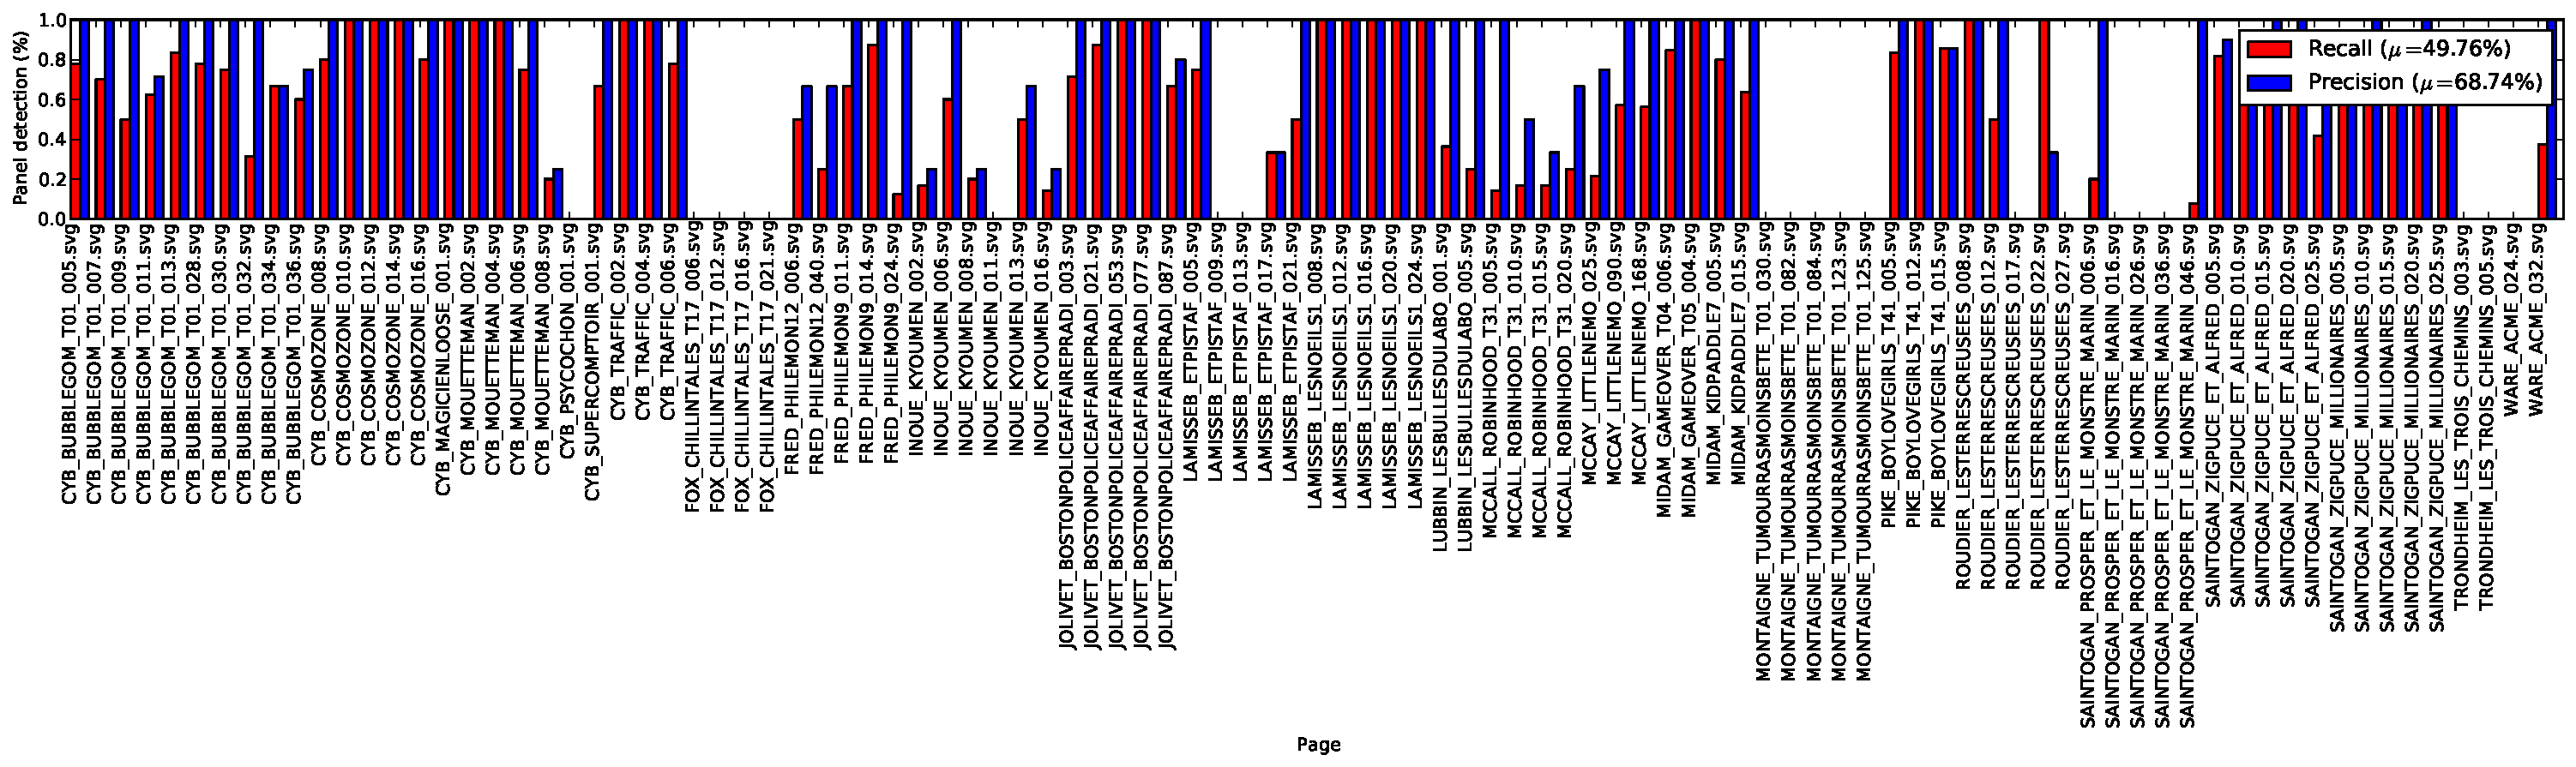
\includegraphics[trim= 0mm 108mm 0mm 0mm, clip, width=\textwidth]{2014-07-20_svg_Ho2012Panel_object.pdf}}
  % \\
  \subfloat[Method A]{\label{fig:ex:text_methodA_extraction_detail}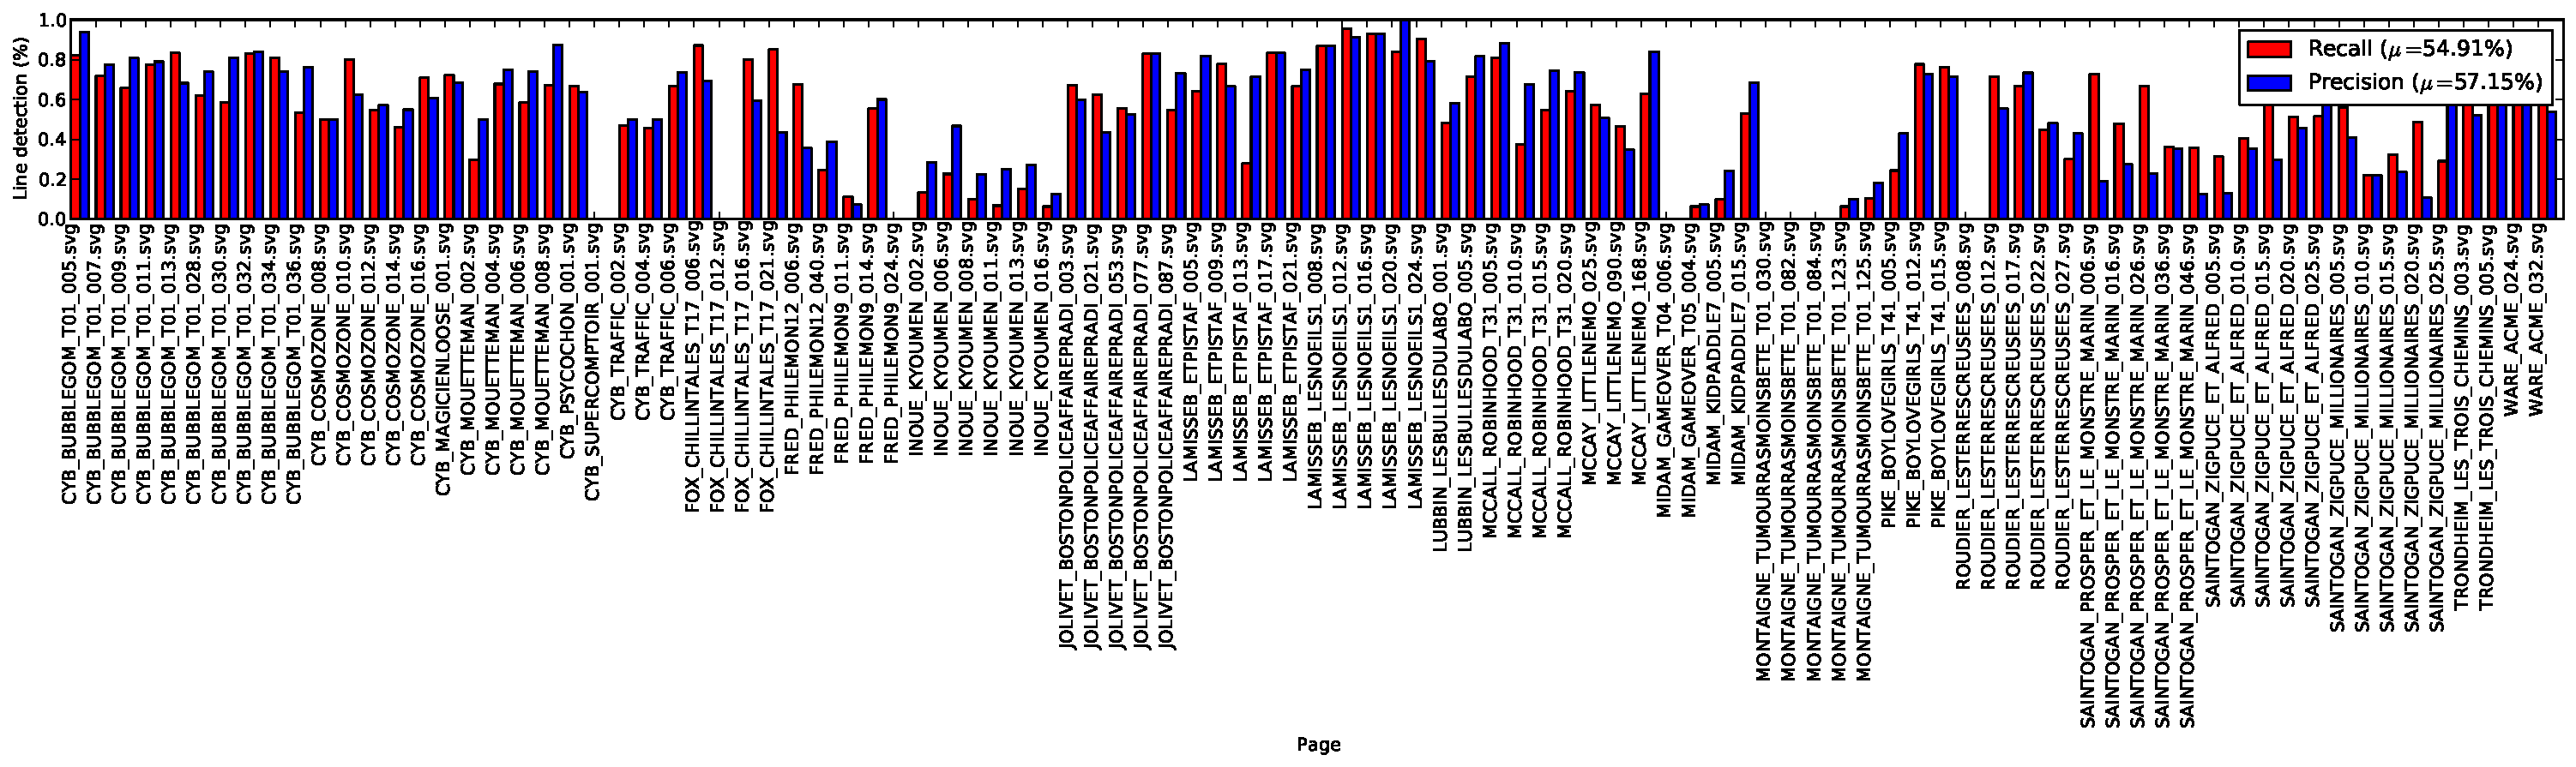
\includegraphics[trim= 0mm 108mm 0mm 0mm, clip, width=\textwidth]{2014-07-24_svg_Rigaud2012LNCS_letter2lineRigaud2014IJDARLine_object.pdf}}
  \\
  \subfloat[Method B using the best bi-level combination method (rgb2grey + Otsu) and OCR]{\label{fig:ex:text_methodB_extraction_detail}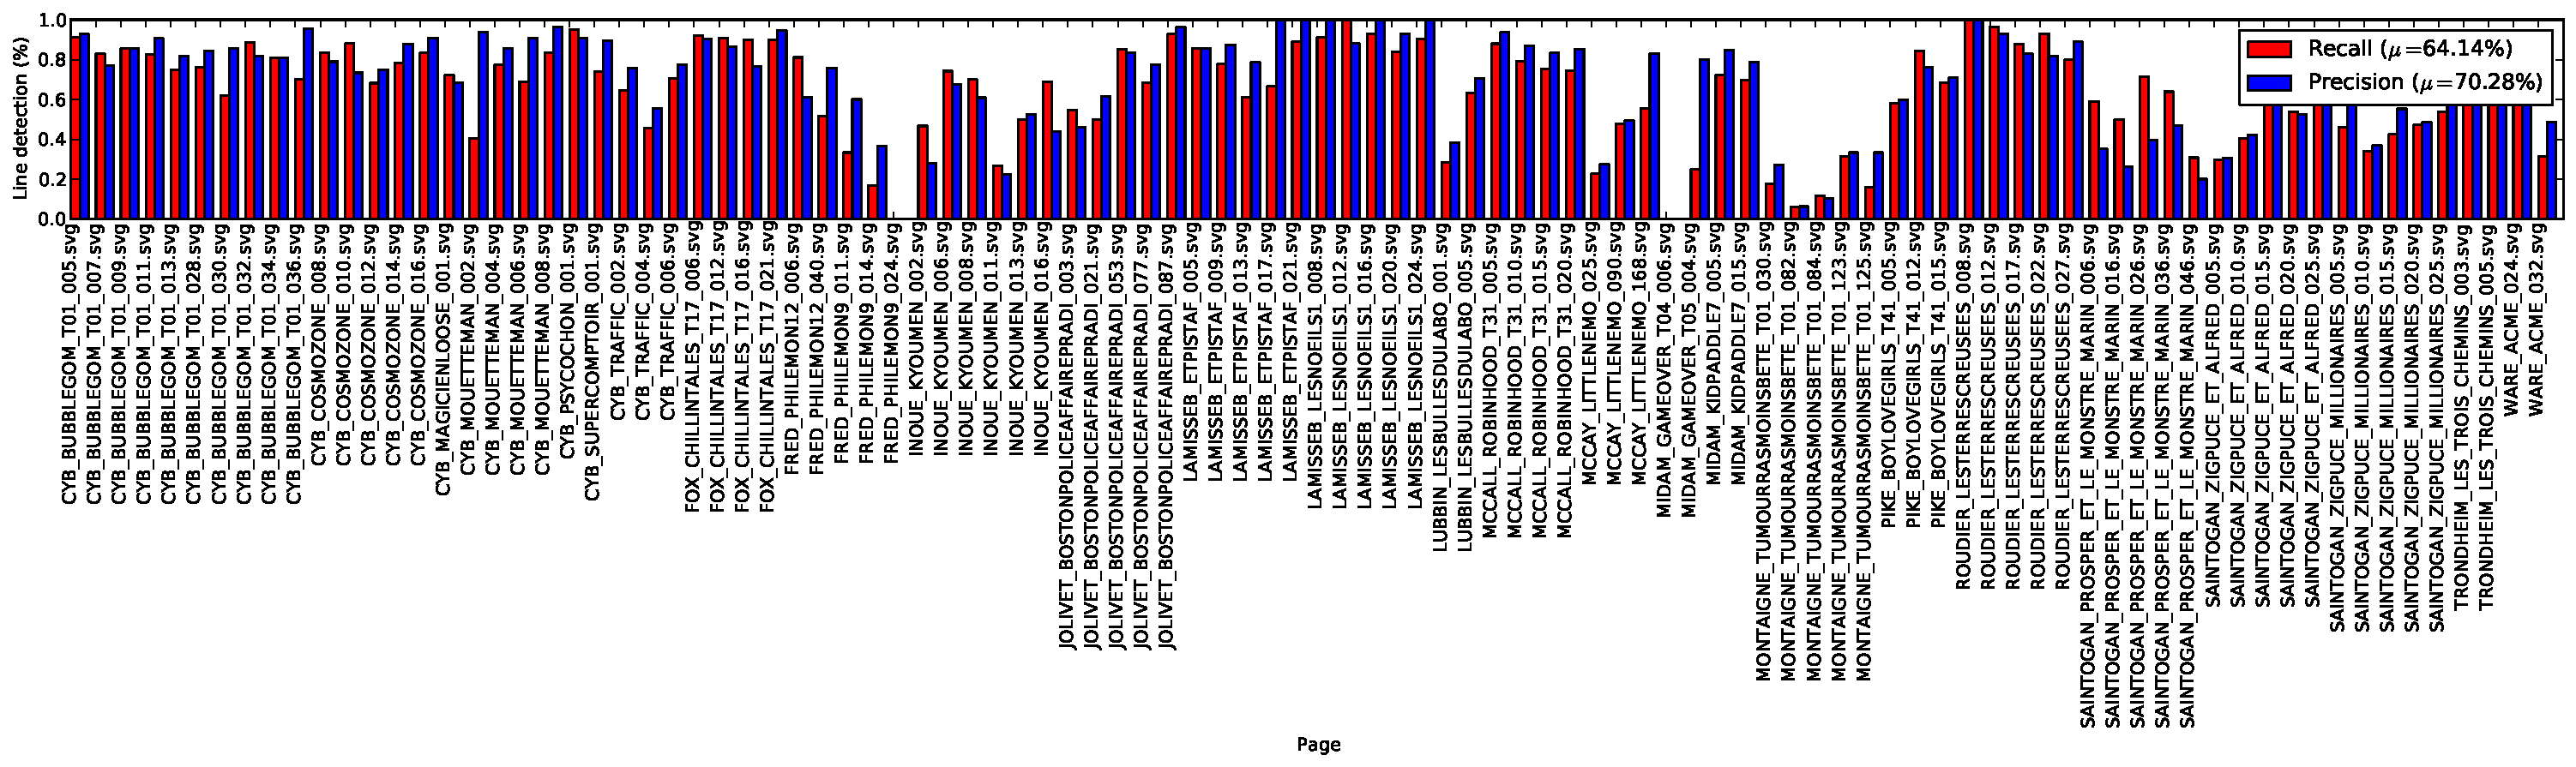
\includegraphics[trim= 0mm 108mm 0mm 0mm, clip, width=\textwidth]{2014-08-19_svg_RigaudVISAPPThesis2014_rgb2gray_otsu_ocr_Line.pdf}}
  \\
  \subfloat[Method C]{\label{fig:ex:text_methodC_extraction_detail}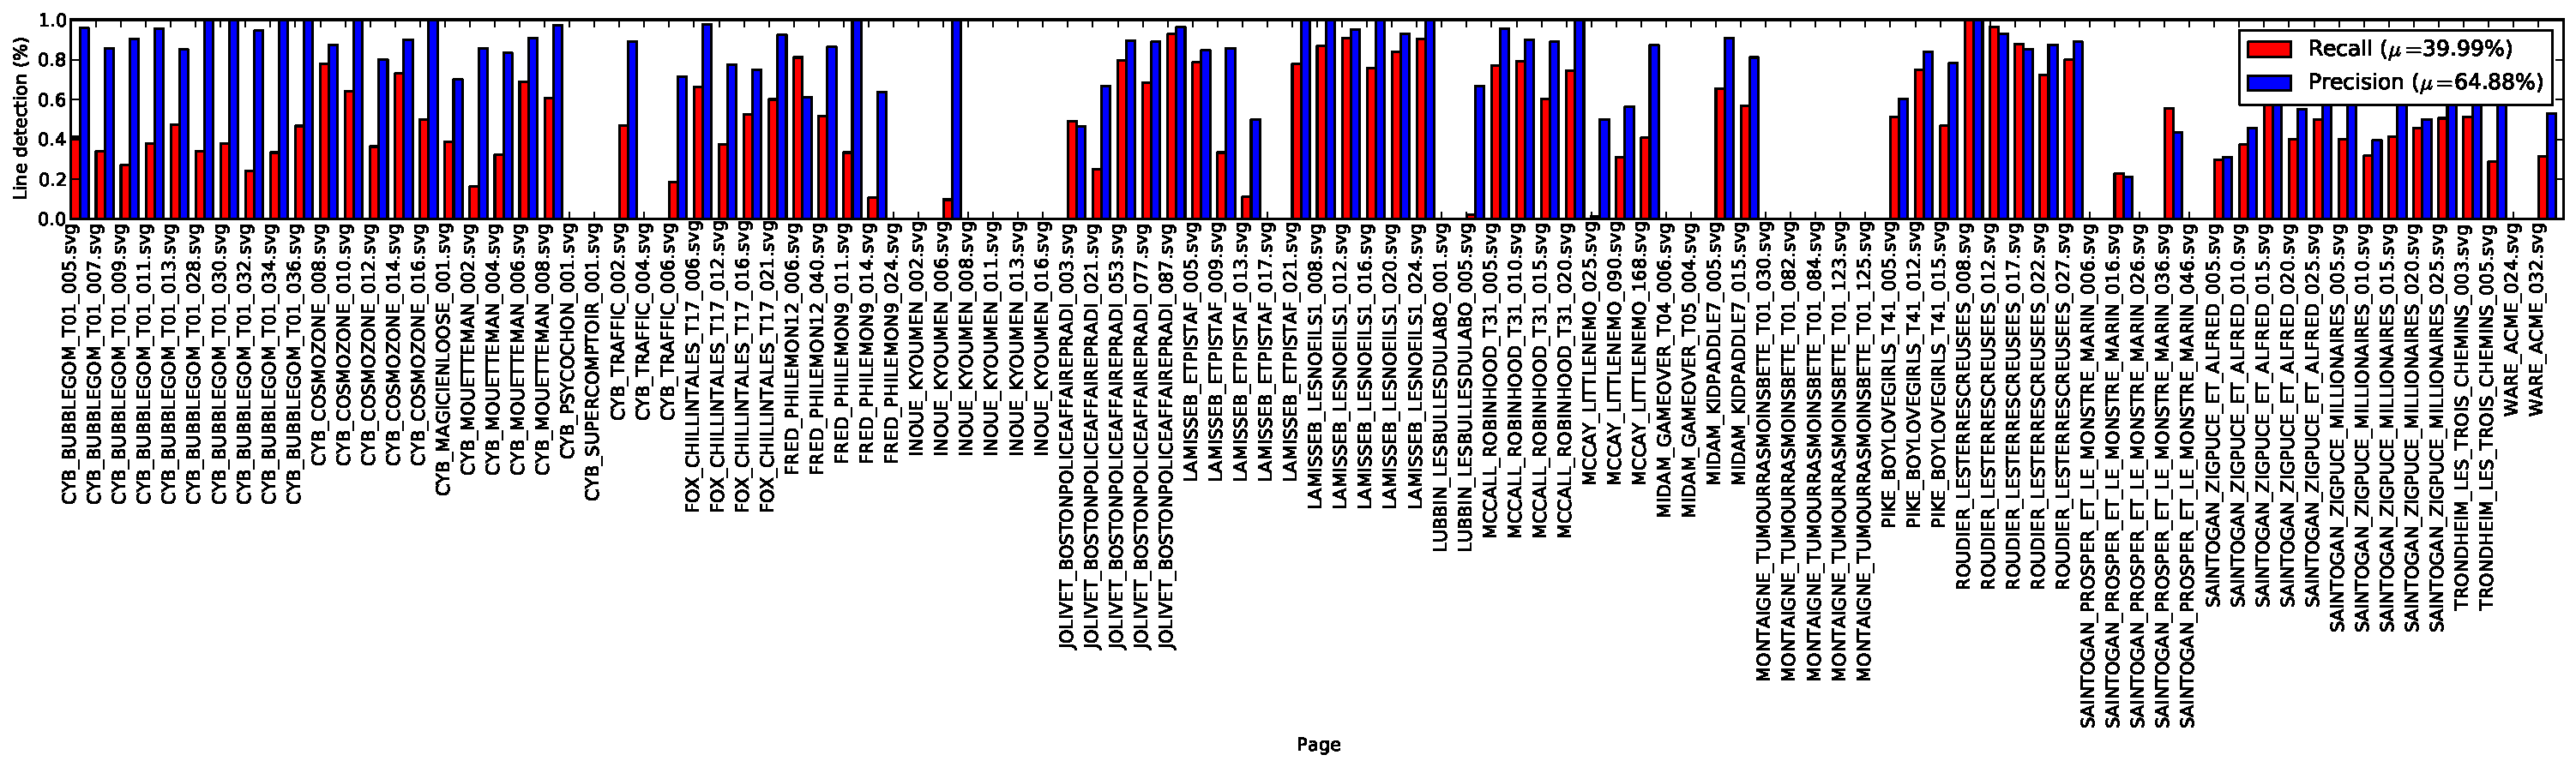
\includegraphics[trim= 0mm 0mm 0mm 0mm, clip, width=\textwidth]{2014-09-04_cleaned_validated_from_method_B_for_panel_text_balloon_and_method_A_for_character_Line.pdf}}

  \caption[Text line extraction score details for each image of the eBDtheque dataset]{Text line extraction score details for each image of the eBDtheque dataset (Appendix~\ref{app:dataset}).}
    \label{fig:ex:text_detection_result_details}
\end{figure}
%%%%%%%%%%%%%%%%%%%%%%%%%%%%%%%%%%%%%%%%%%%%%%%%%%%

\section{Text recognition evaluation} % (fold)
\label{par:ex:text_recognition_evaluation}
% \paragraph{Text recognition evaluation} % (fold)
% \label{par:ex:text_recognition_evaluation}

We evaluated text transcription using string edit distance between a predicted text transcription given by the OCR and its corresponding transcription in the ground truth (Section~\ref{sub:ex:text_recognition_metric}).
The eBDtheque dataset is composed of English, Japanese and French texts.
We evaluated the transcription given by the OCR engine Tesseract version 3.02.02 with the provided training data for each language\footnote{\url{https://code.google.com/p/tesseract-ocr/downloads/list}}.
% corresponding to the language defined in the ground truth of each image of the dataset.
This was performed at the text line level, taking as correct the text lines that were transcribed exactly as the ground truth transcription, ignoring case (lower/upper case) and accents for predicted and ground truth regions.
% with a edit distance $<$ 10\% of their length using equation~\ref{eq:recall} and~\ref{eq:precision}.
%For instance a recognised text line of ten elements will be considered as correct if less than three are split, deleted, transposed, replaced or inserted. 
Table~\ref{tab:ex:text_recogniton_results} shows text recognition results given the text line position from the ground truth (best reachable score) and from the best automatic text localisation method (Method I in Table~\ref{tab:text_results}).

    %%%%%%%%%%%%%%%%%%%%%%%%%%%%%%%%%%%%%%%%%%%%%%%%%%%
  \begin{table}[ht]
    % \normalsize
    \centering
    \caption{Text recognition accuracy $A_{textReco}$ results from automatic text line localisation at an edit distance ($ED$) of 0, 1 and 2.}
    \begin{tabular}{|c|c|c|c|}
          \hline
          Text extraction method &  $ED=0$  & $ED=1$  & $ED=2$  \\
          \hline
          % Ground truth  & \modif{??}   & \modif{??} & \modif{??}       \\
          % \hline
          Method B  &  11.11  & 16.53     & 20.67       \\
          \hline
        \end{tabular}
    \label{tab:ex:text_recogniton_results}
  \end{table}%
    %%%%%%%%%%%%%%%%%%%%%%%%%%%%%%%%%%%%%%%%%%%%%%%%%%%

We obtained a score of $A_{textReco}=11.11\%$ for perfect transcription from the automatic text extraction and OCR method which constitute a baseline for future work on text recognition on the eBDtheque dataset~\cite{Guerin2013}.
Table~\ref{tab:ex:text_recogniton_results} shows the results for a more relaxed evaluation where we also considered as correct the text lines at a text edit distance equal to one and two, the accuracy rise up to 20.67\%.
%The distribution of the text line lengths is given in Figure~\ref{fig:textline_lenth_distribution}.
Note that the average text line length is quite short in comic books compared to other documents, the distribution is given Figure~\ref{fig:ex:textline_lenth_distribution}.

% subsection results_analysis (end)



\section{Balloon extraction evaluation} % (fold)
\label{sub:ex:balloon_extraction_evaluation}
In this section we evaluate our three balloon extraction approaches (Method S, I and K) and compare them to two methods from the literature.
We compare our results to Arai~\cite{Arai10} and Ho~\cite{Ho2012} that are two state of the art methods (Section~\ref{sec:sota:layout_panel}).
% The first one uses connected-component analysis similarly to our proposition and the second is based on region growing.
The evaluations are performed on the 1091 balloons of the eBDtheque dataset~\cite{Guerin2013} at object and pixel levels in order to provide a performance evaluation for localisation and contour analysis purposes (Sections~\ref{sub:ex:object_localisation_metric} and~\ref{sub:ex:object_segmentation_metric}).
%also measure the impact on the balloon classification based on balloon's contour analysis.
% We evaluate the three approaches on the 1092 balloons of the eBDtheque dataset~\cite{Guerin2013} at object bounding box and pixel levels, and compare to previous work from the literature.
% We also evaluate the tail detection for each balloon extraction approaches

In the eBDtheque ground truth, 84.5\% of the balloons are closed and 15.5\% are not (implicit).
Thus we do not expect to reach 100\% recall and precision for the regular balloon extraction methods because they are not designed for implicit balloons.
One the other hand, implicit balloon extraction method is able to extract closed balloon as well.

% \subsection{Experimental settings} % (fold)
% % \label{sub:experimental_settings}

% TODO

\subsection{Arai's method} % (fold)
\label{sub:ex:balloon_extraction_arai}

Arai's method in a sequential method that extracts balloon inside panel regions in order to extract text inside~\cite{Arai11}.
It it similar to its panel extraction work-flow also presented in the same paper (Section~\ref{sub:ex:panel_extraction_arai}), without image inversion which basically detect white blobs (assuming speech balloons have a white background).
Not all the white blobs correspond to balloons in the comic book images, especially for the monochrome ones.
The method selects blob candidates according to four rules based on blob size, white pixel occurrence, vertical straight line detection and width to length ratio.
We re-implemented all the rules and heuristics of the original paper except for the straight line detection that we rotated of 90 degrees for images using horizontal text.

The score of this method  was in average for recall and precision of 13.40\% and 11.76\% (Figure~\ref{fig:ex:balloon_arai_extraction_detail}).

% %%%%%%%%%%%%%%%%%%%%%%%%%%%%%%%%%%%%%%%%%%%%%%%%%%%%%%
% \begin{figure}[h]
%  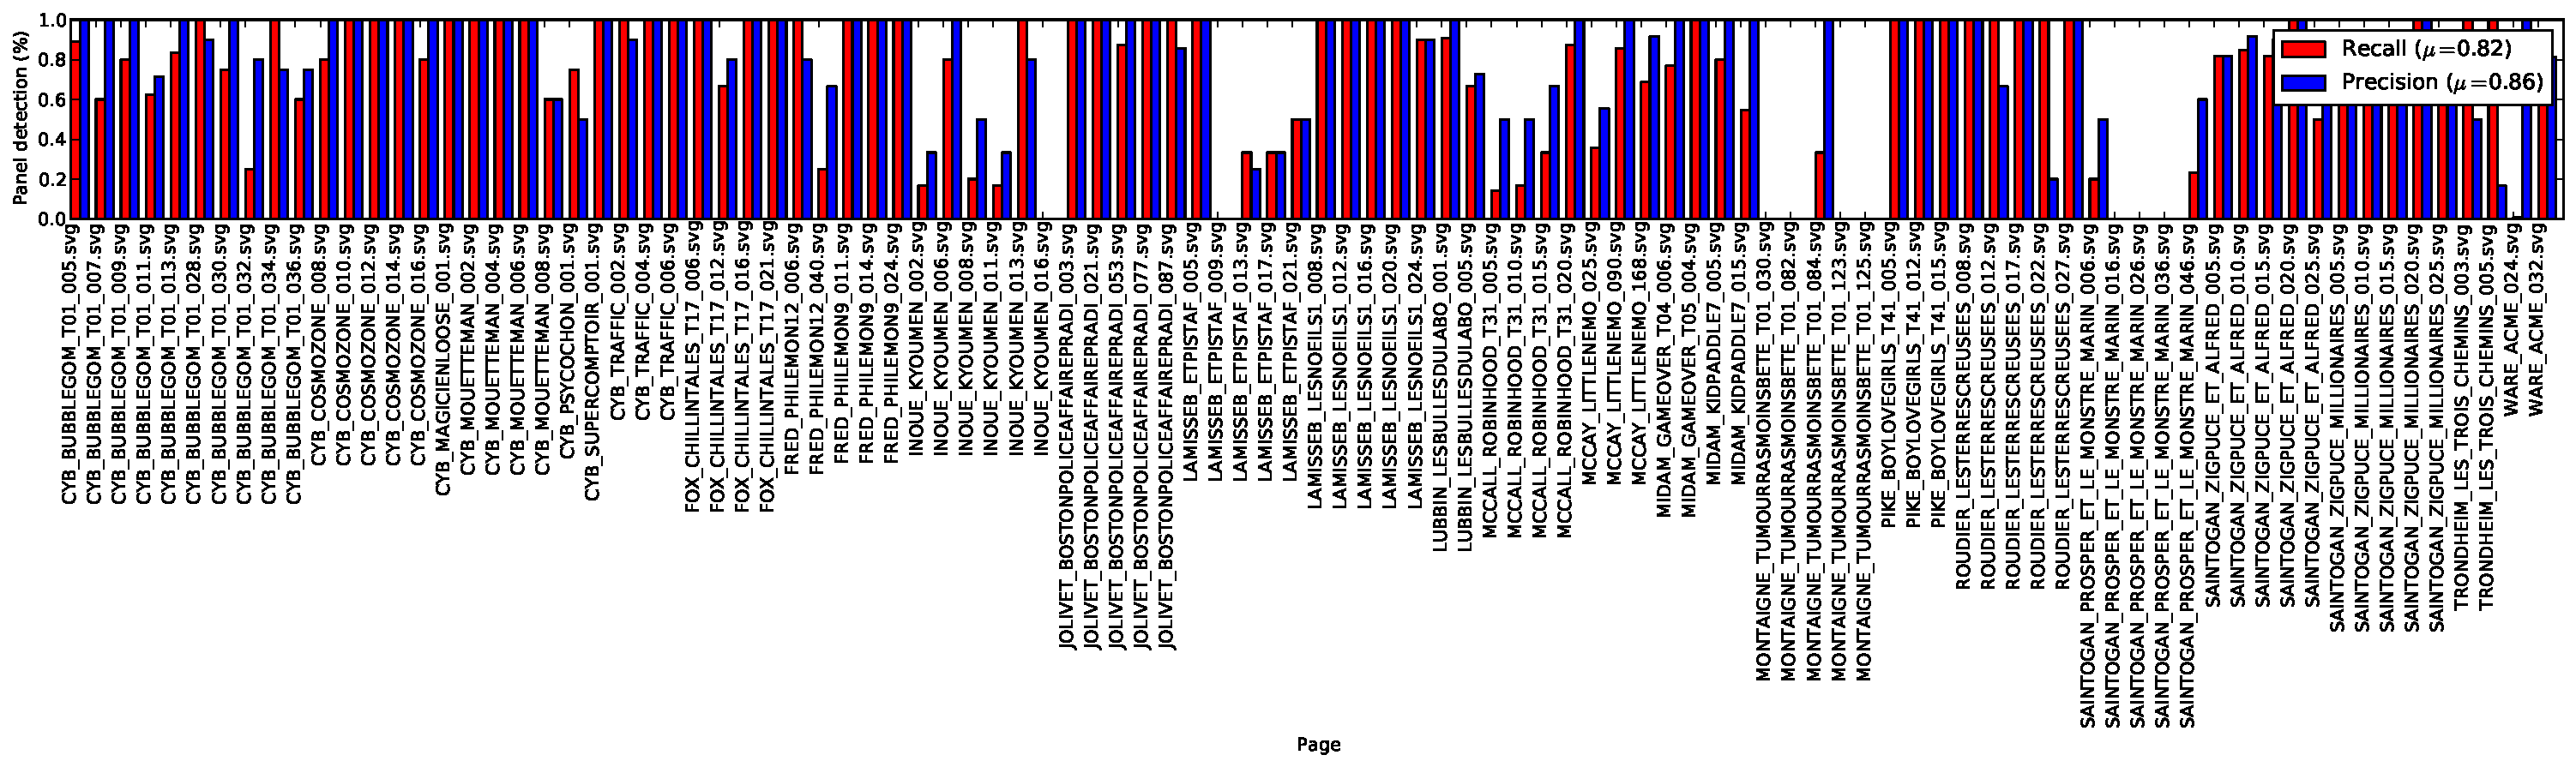
\includegraphics[width=\textwidth,height=4cm]{Panel_object_proposed.pdf}
%  \caption{Balloon extraction score details of Arai's method for each image of the eBDtheque dataset \modif{TODO: update}.
%  }
%  \label{fig:ex:balloon_arai_extraction_detail}
% \end{figure}
% %%%%%%%%%%%%%%%%%%%%%%%%%%%%%%%%%%%%%%%%%%%%%%%%%%%%%%

% subsection arai_s_method_cite (end)

\subsection{Ho's method~\cite{Ho2012}} % (fold)
% \label{sub:arai_s_method_cite}

Ho's method is a sequential approach, similarly to Arai's approach, that extracts balloon inside panel regions in order to extract text inside~\cite{Ho2012}.
First it converts the image from RBG to HSV colour representation and select candidate regions with a high value (V) and low saturation (S) level.
To reduce the number of candidate regions, a second selection is applied according to size and shape.
Small regions are removed and only regions with a ratio between the number of pixel in the region over the number of pixel in its bounding higher than 60\% are kept.
In the original paper, only the ratio between the region area and its bounding box was given (60\%).
Low value (V) and high saturation (S) values were not mentioned in the original paper, we decided to combine them by removing the value (V) from the saturation (S) to compute a brightness level $B=S-V$ in order to reduce the number of parameters.
We fixed $B=200$, only region with a higher brightness level are kept.
We considered as small regions the region with a width or height inferior to three pixels.

The score of this method  was in average for recall and precision of 13.96\% and 24.73\% (Figure~\ref{fig:ex:balloon_ho_extraction_detail}).

%%%%%%%%%%%%%%%%%%%%%%%%%%%%%%%%%%%%%%%%%%%%%%%%%%%%%%
% \begin{figure}[h]
%  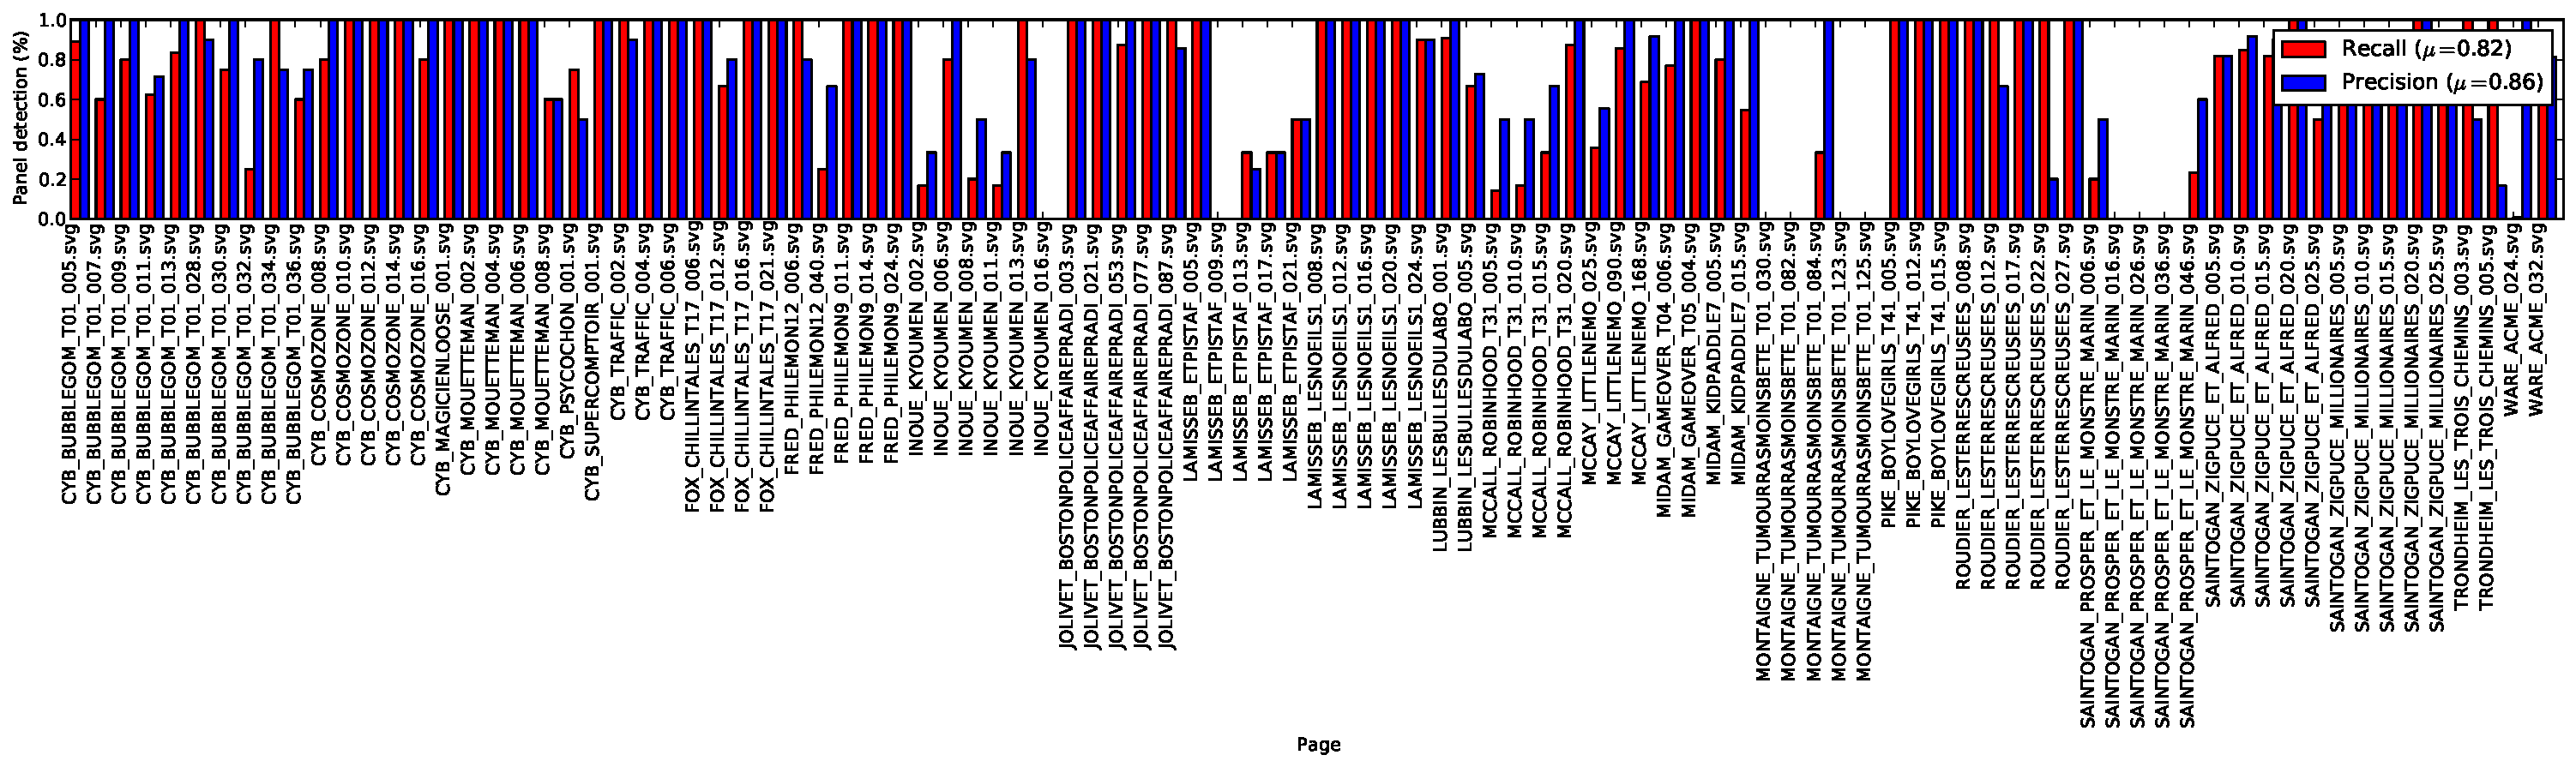
\includegraphics[width=\textwidth,height=4cm]{Panel_object_proposed.pdf}
%  \caption{Balloon extraction score details of Ho's method for each image of the eBDtheque dataset \modif{TODO: update}.
%  }
%  \label{fig:ex:balloon_ho_extraction_detail}
% \end{figure}
%%%%%%%%%%%%%%%%%%%%%%%%%%%%%%%%%%%%%%%%%%%%%%%%%%%%%%

% TODO: describe the method here? Ho's method is a sequential approach that search for panel first and then balloon inside panels and text inside balloons.
% The parameter used in the experiment are not given, I propose mine...

% subsection ho_s_method_cite (end)

\subsection{Sequential approach} % (fold)
% \label{sub:method_a}

In Sections~\ref{sub:se:regular_balloon_extraction} and~\ref{sub:se:implicit_balloon_extraction} we have presented two sequential approaches for regular and implicit balloon extraction from text line positions.
Here, we evaluated them separately and detail the benefits of energies used for implicit balloon extraction by active contour model.
For both regular and implicit balloon extraction, the input text is given from the sequential text extraction method (Section~\ref{sec:se:panel_and_text}) since it is the previous step of this approach.

\paragraph{Regular balloons} % (fold)
\label{par:regular_balloons}

Regular balloon extraction method is based on a white blob selection according to the central position of text lines in the balloon.
This central position is converted as confidence value $C_{balloon}$ for each balloon candidate.
The evolution of the performance of recall and precision according to this confidence rejection criterion is plotted Figure~\ref{fig:ex:validation_confidence_balloon_methodA_regular}.
The best score of $R=37.25\%$ and $P=45.19\%$ was obtained for \modif{$C_{balloon} > 10\%$} (Figure~\ref{fig:ex:closed_balloon_methodA_extraction_detail}).


%%%%%%%%%%%%%%%%%%%%%%%%%%%%%%%%%%%%%%%%%%%%%%%%%%%%%%
\begin{figure}[h]
  \centering
 
\includegraphics[width=0.7\textwidth]{figure_here.png}
 \caption{Validation of the regular balloon confidence value for Method A.
 }
 \label{fig:ex:validation_confidence_balloon_methodA_regular}
\end{figure}
%%%%%%%%%%%%%%%%%%%%%%%%%%%%%%%%%%%%%%%%%%%%%%%%%%%%%%


%%%%%%%%%%%%%%%%%%%%%%%%%%%%%%%%%%%%%%%%%%%%%%%%%%%%%%
% \begin{figure}[h]
%  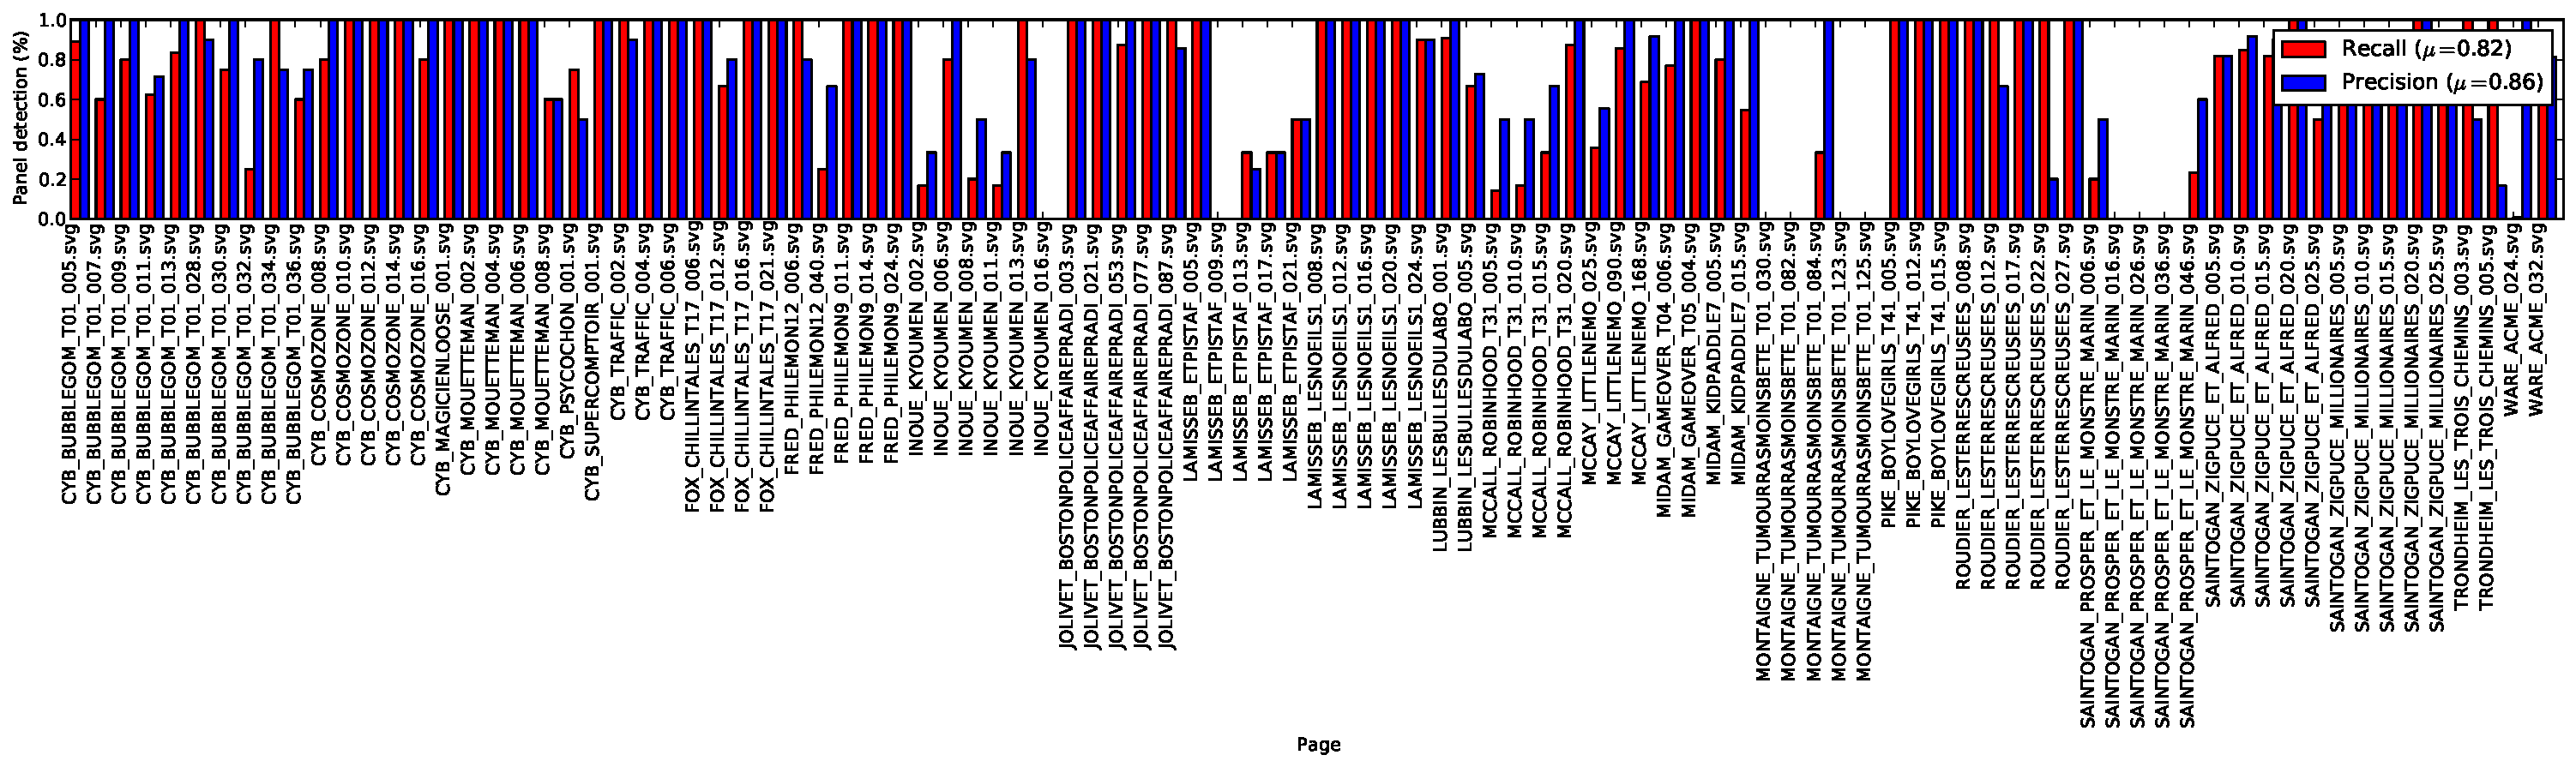
\includegraphics[width=\textwidth,height=4cm]{Panel_object_proposed.pdf}
%  \caption{Balloon extraction score details of Method A for each image of the eBDtheque dataset \modif{TODO: update}.
%  }
%  \label{fig:ex:balloon_methodA_extraction_detail}
% \end{figure}
%%%%%%%%%%%%%%%%%%%%%%%%%%%%%%%%%%%%%%%%%%%%%%%%%%%%%%

%We consider as correctly detected the balloon with a confidence value higher than \modif{10\%} (Table~\ref{tab:ex:balloon_localisation_comparison_results}, Method A (1)).

% paragraph regular_balloons (end)


\paragraph{Implicit balloons} % (fold)
\label{par:ex:implicit_balloons_reminder}

The implicit balloon extraction method was evaluated using three different scenarios in order to highlight the benefits of both active contour theory and domain specific knowledge.
% that considers as balloon any white connected components that overlaps at more than $10\%$ with text regions.
First, the performance using active contour model with only the internal energy, then with the distance transform based external energy described section~\ref{sec:se:external_energie} and third, we added the domain knowledge energy $E_{text}$ from Section~\ref{sec:se:text_energie} (Table~\ref{tab:ex:implicit_balloon_performance_object_pixel_comparison}).
The best score for object level detection ($R=57.76\%$ and $P=41.62\%$) are detailed for each image of the dataset in Figure~\ref{fig:ex:implicit_balloon_methodA_extraction_detail}.

% Fourth, after a two stage contour fitting (4).
% Results are presented in table~\ref{tab:ex:balloon_localisation_comparison_results}.


%%%%%%%%%%%%%%%%%%%%%%%%%%%%%%%%%%%%%%%%%%%%%%%%%%
\begin{table}[h]
  \normalsize
% \renewcommand{\arraystretch}{1.3}
% \extrarowheight as needed to properly center the text within the cells
  \centering
  \caption{Implicit balloon performance evaluation at object and pixel levels using the original form and the proposed (with $E_{text}$) energy functions.}
  \begin{tabular}{|c|c|c|c|c|c|c|}
  \hline
    & \multicolumn{3}{|c|}{Object level}  & \multicolumn{3}{|c|}{Pixel level}   \\
  \hline
  Energy function  &  $ R$ (\%)  & $P$ (\%)& $F$ (\%)   &  $R$ (\%)  & $P$ (\%)   & $F$ (\%)\\
  \hline
%   Ho~\cite{Ho2012}  & ???     & ???   & & ???     & ???&    \\

  %$E = E_{int}$     & \modif{???}       & \modif{???}     & \modif{???}       & \modif{???}  & \modif{???} & \modif{???}   \\
  %\hline
   $E = E_{int} + E_{ext}$    & 56.01       & 40.40     & 46.94       & 69.40  & \textbf{83.98} & 76.00   \\
  \hline
  $E = E_{int} + E_{ext} + E_{text}$   & \textbf{57.76} & \textbf{41.62} & \textbf{48.38} & \textbf{74.80} & 82.67 & \textbf{78.55}    \\
  \hline
  \end{tabular}
      \label{tab:ex:implicit_balloon_performance_object_pixel_comparison}
\end{table}%
    %%%%%%%%%%%%%%%%%%%%%%%%%%%%%%%%%%%%%%%%%%%%%%%%%%%

% paragraph implicit_balloons (end)

%, the recall $R=??\%$, precision $P=?\%$ and f-measure $F=?\%$.

% subsection method_a (end)
\subsection{Independent approach} % (fold)
% \label{sub:method_b}

We introduced Method I in Section~\ref{sub:in:balloon_segmentation}, it is a independent approach that does not require any previous other element extraction.
This method requires one parameter which is the minimum number of children $minNbChildren$ of a balloon (number of included connected-components).
We set $minNbChildren=8$ according to the parameter validation, just before the first peak in the distribution of the number of letters per speech balloon (Figure~\ref{fig:ex:min_number_children_validation}).
Note that in Figure~\ref{fig:ex:min_number_children_validation}, there are about 3.5\% of the balloons below the selected threshold that contain one or two letters, usually punctuation marks.
%such as ``?'' or ``!''. 
We voluntary omitted them here to avoid detecting a lot of non balloon regions.

    %%%%%%%%%%%%%%%%%%%%%%%%%%%%%%%%%%%%%%%%%%%%%%%%%%%%%%%%
    \begin{figure}[h]%trim=l b r t  width=0.5\textwidth,  
      \centering
      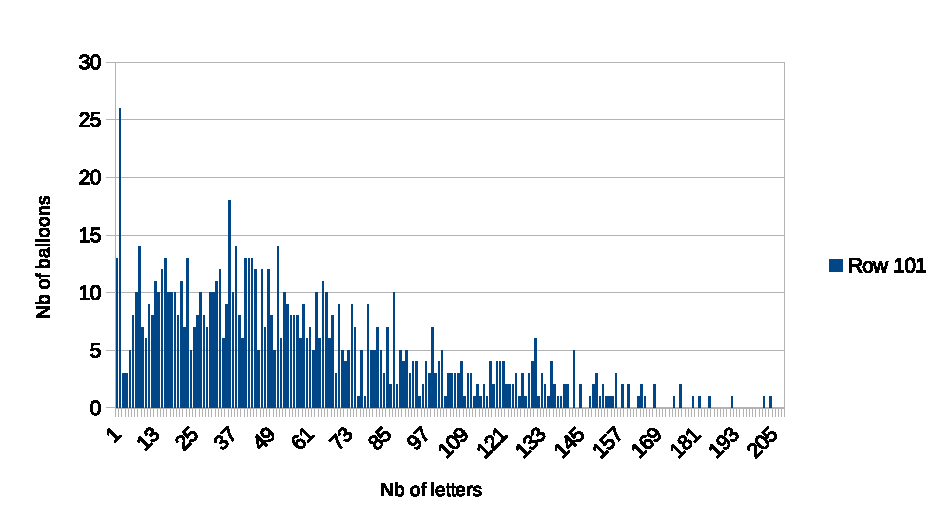
\includegraphics[trim= 10px 0px 60px 0px, clip, width=0.75\textwidth]{number_of_letter_per_balloon.pdf}
      \caption[Distribution of the number of letter per speech balloon]{Distribution of the number of letter per speech balloon in the eBDtheque dataset~\cite{Guerin2013}.
      }
      \label{fig:ex:min_number_children_validation}
    \end{figure}  
    %%%%%%%%%%%%%%%%%%%%%%%%%%%%%%%%%%%%%%%%%%%%%%%%%%%%%%%%

% Balloons with a confidence value $C_{balloon}$ lower than 10\% were rejected according to the validation experiments on the eBDtheque dataset~\cite{Guerin2013}.

This regular balloon extraction method attributes a confidence value $C_{balloon}$ to each balloon candidate according to the alignment of the connected-components it contains (children), similarly to regular balloon extraction of Method S.
The evolution of the performance of recall and precision according to this confidence rejection criterion is plotted Figure~\ref{fig:ex:validation_confidence_balloon_methodB_regular}.
The best score of $R=52.68\%$ and $P=44.17\%$ was obtained for \modif{$C_{balloon} > 50\%$}, details are given Figure~\ref{fig:ex:balloon_methodB_extraction_detail}.
Figure~\ref{fig:ex:balloon_methodB_extraction_detail} confirms that our method works best when the balloons are closed, well segmented and with non cursive text inside.

%%%%%%%%%%%%%%%%%%%%%%%%%%%%%%%%%%%%%%%%%%%%%%%%%%%%%%
\begin{figure}[h]
  \centering
 
\includegraphics[width=0.7\textwidth]{figure_here.png}
 \caption{Validation of the regular balloon confidence value for Method I.
 }
 \label{fig:ex:validation_confidence_balloon_methodB_regular}
\end{figure}
%%%%%%%%%%%%%%%%%%%%%%%%%%%%%%%%%%%%%%%%%%%%%%%%%%%%%%


%%%%%%%%%%%%%%%%%%%%%%%%%%%%%%%%%%%%%%%%%%%%%%%%%%%%%%
% \begin{figure}[h]
%  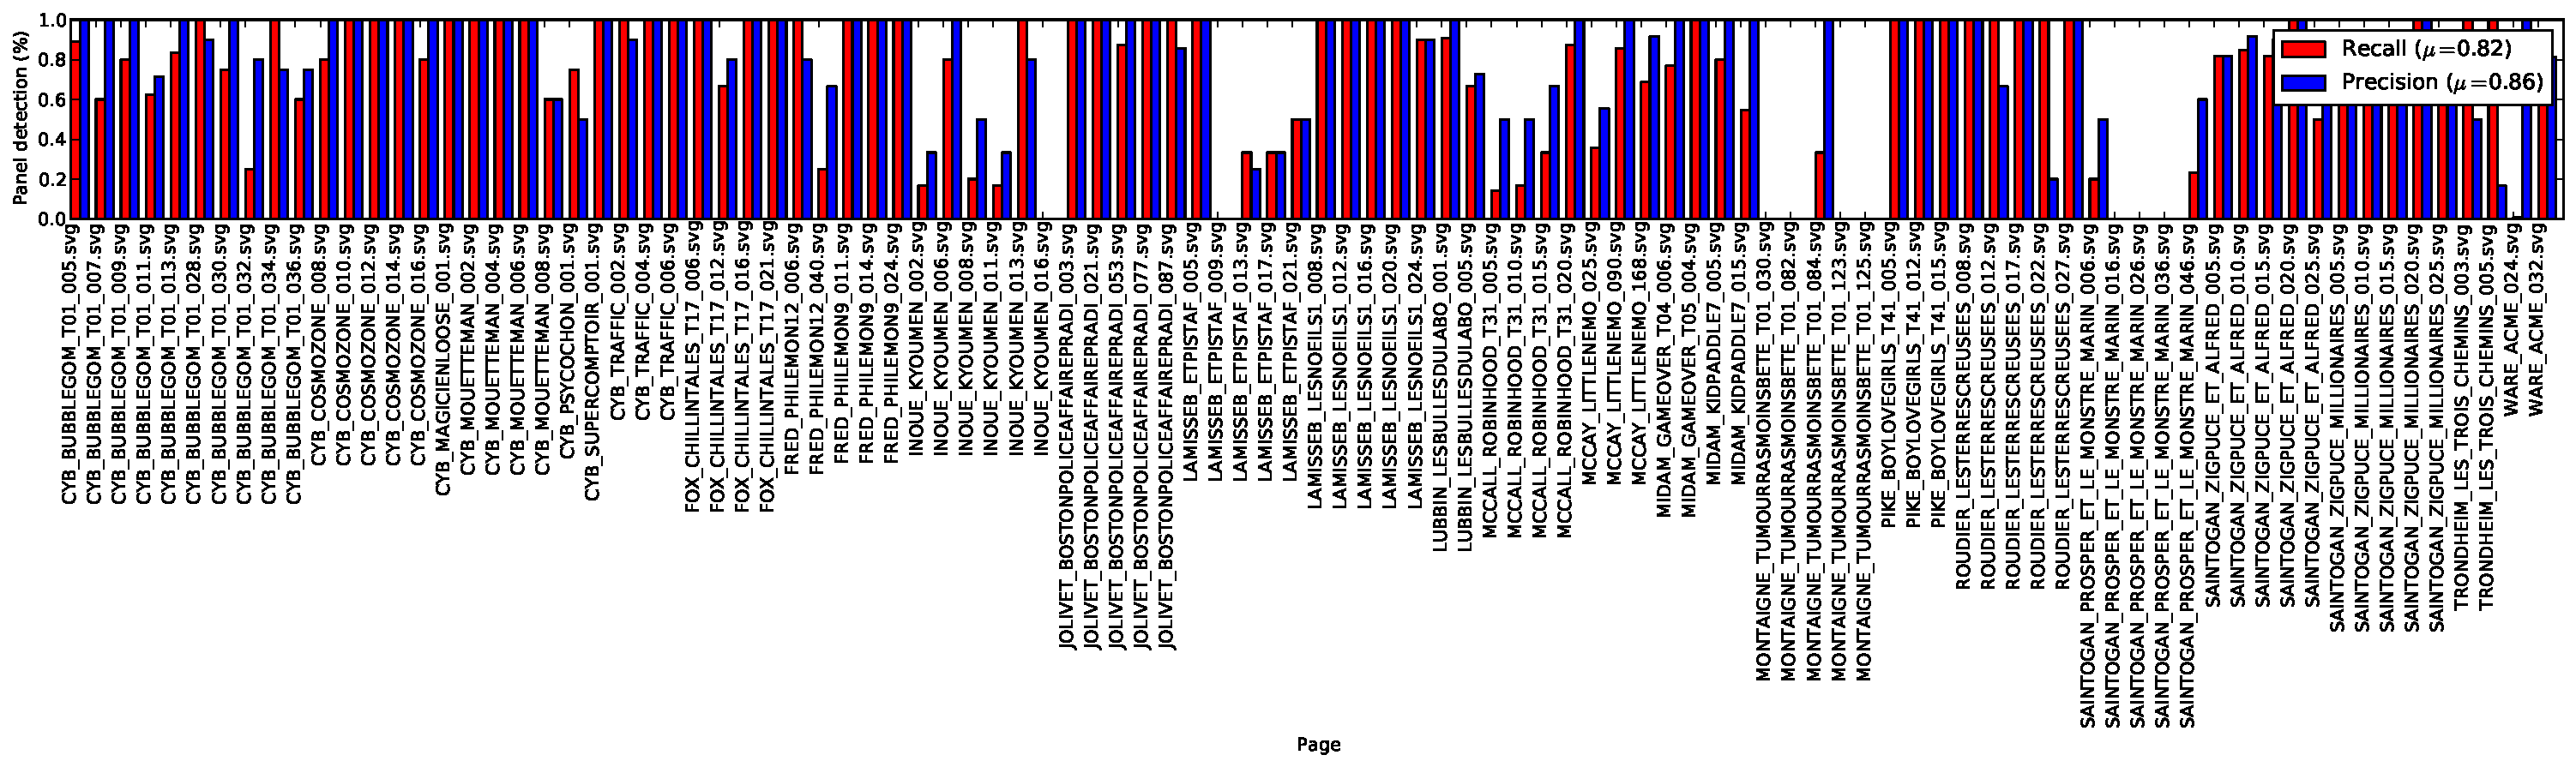
\includegraphics[width=\textwidth,height=4cm]{Panel_object_proposed.pdf}
%  \caption{Balloon extraction score details of Method B for each image of the eBDtheque dataset \modif{TODO: update}.
%  }
%  \label{fig:ex:balloon_methodB_extraction_detail}
% \end{figure}
%%%%%%%%%%%%%%%%%%%%%%%%%%%%%%%%%%%%%%%%%%%%%%%%%%%%%%


% subsection method_b (end)
\subsection{Knowledge-driven approach} % (fold)
% \label{sub:method_c}

The knowledge-driven approach can be used as a post processing of the balloon extraction.
It validates or rejects balloon candidates according to contextual information from the proposed model (Section~\ref{sec:kn:processing_sequence}).
In the model, the rules concerning balloon are that they should be contained in a panel and not contain other balloon, panel or comic character.
Considering the best method for balloon extraction (Method S implicit in Table~\ref{tab:ex:balloon_localisation_comparison_results}), the score of this method was in average for recall and precision of 39.56\% and 48.65\% (Figure~\ref{fig:ex:balloon_methodC_extraction_detail}).

%%%%%%%%%%%%%%%%%%%%%%%%%%%%%%%%%%%%%%%%%%%%%%%%%%%%%%
% \begin{figure}[h]
%  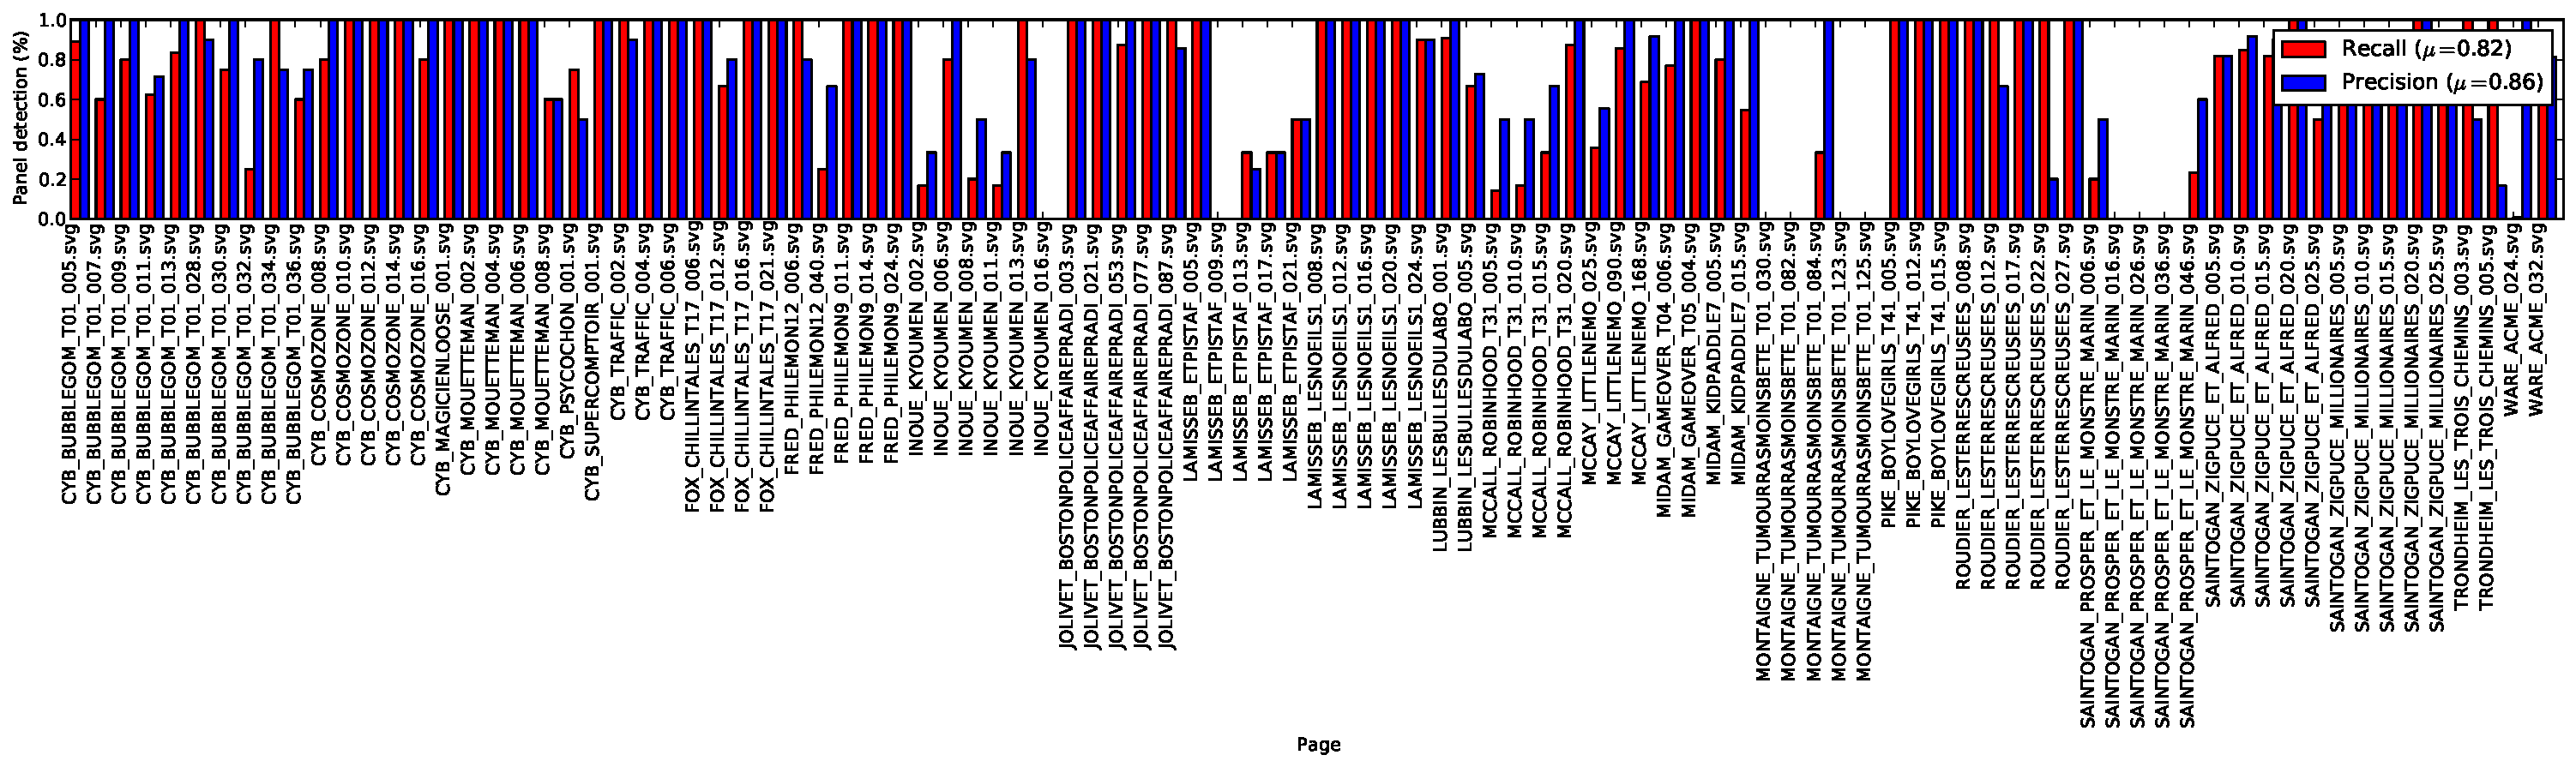
\includegraphics[width=\textwidth,height=4cm]{Panel_object_proposed.pdf}
%  \caption{Balloon extraction score details using Method C for each image of the eBDtheque dataset \modif{TODO: update}.
%  }
%  \label{fig:ex:balloon_methodC_extraction_detail}
% \end{figure}
%%%%%%%%%%%%%%%%%%%%%%%%%%%%%%%%%%%%%%%%%%%%%%%%%%%%%%

% subsection method_c (end)
% subsection experimental_settings (end)




\subsection{Comparison and analysis} % (fold)
% \label{sub:result_analysis}


% In this section, we discuss balloon localisation at bounding box and pixel levels, and also balloon classification.


% subsection result_analysis (end)

% \paragraph{Regular balloons} % (fold)
% \label{par:regular_balloons}

% paragraph regular_balloon (end)
% The second method for regular balloon extraction presented Section~\ref{sub:in:balloon_segmentation}
% The recall and precision scores are given Figure~\ref{fig:ex:regular_balloon_extraction} according to the confidence value $C_{balloon}$.


  %%%%%%%%%%%%%%%%%%%%%%%%%%%%%%%%%%%%%%%%%%%%%%%%%%%
  % \begin{figure}[h!]  %trim=l b r t  width=0.5\textwidth,
  %   \centering
  %   
\includegraphics[trim= 0px 0px 0px 0px, clip, width=0.75\textwidth]{figure_here.png}
  %   \caption[Regular balloon extraction results]{Regular balloon extraction results.}
  %   \label{fig:ex:regular_balloon_extraction}
  % \end{figure}
  %%%%%%%%%%%%%%%%%%%%%%%%%%%%%%%%%%%%%%%%%%%%%%%%%%%



% \paragraph{Implicit balloons} % (fold)
% \label{par:implicit_balloons}

% We evaluated our different contributions separately.
% First we measured balloon localization performance at bounding
% box level to highlight the benefits of both active contour theory
% and domain specific knowledge.
% Second, we performed pixel level evaluation on a smaller subset to show the ability of our method to fit balloon contour details.

% In order to provide a comparative analysis we attempted comparison to the methods of Arai~\cite{Arai11} and Ho~\cite{Ho2012}, which are based on connected component detection and filtering. Unfortunately, direct comparison to these methods is not possible as Arai's approach~\cite{Arai11} is based on two rules specifically designed for Japanese manga comics with vertical text and Ho~\cite{Ho2012} is based on growing region segmentation which is not appropriate for open balloon detection neither.
% We also compared to the original active contour implementation proposed by Kass et al.~\cite{Kass1988} but because the initialization is not close enough to the edges, the internal energies make the snake retracts on itself.

% We compare our results using four different scenarios.
% First with the regular balloon extraction method presented just above (1).
% % that considers as balloon any white connected components that overlaps at more than $10\%$ with text regions.
% Second, the active contour with the distance transform based external energy described section~\ref{sec:external_energie} (2) and third, we add the domain knowledge energy $E_{text}$ (3) from Section~\ref{sec:text_energie}.
% Fourth, after a two stage contour fitting (4).
% Results are presented in table~\ref{tab:ex:balloon_localisation_comparison_results}.
% For each method, we present two variants, one making use of ground truth localization for the text areas as seeds for balloon localization, and another making use the results of the automatic text localization method presented Section~\ref{sec:se:panel_and_text}.

% \paragraph{Balloon localisation} % (fold)
% \label{par:balloon_localisation}
Balloon localisation aims to evaluate how the presented methods are good at predicting where the balloons are in the image.
Object localisation are performed at the level of object bounding box (Section~\ref{sub:ex:object_localisation_metric}).
Table~\ref{tab:ex:balloon_localisation_comparison_results} compares the average results we obtained for the best performance of the three proposed methods and two methods from the literature.

% paragraph balloon_localisation (end)
% Table~\ref{tab:text_results} summarises the recall, precision and f-measure of the experimented methods.

    %%%%%%%%%%%%%%%%%%%%%%%%%%%%%%%%%%%%%%%%%%%%%%%%%%%
  % \begin{table}[ht]
  %   % \normalsize
  %   \centering
  %   \caption{Balloon localisation result summary.}
  %   \begin{tabular}{|c|c|c|c|}
  %         % \hline
  %         %   & \multicolumn{2}{|c|}{Character 1}   & \multicolumn{2}{|c|}{Character 2}   \\
  %         \hline
  %         &  $R$ (\%)  & $P$ (\%)  & $F$ (\%)  \\
  %         \hline
  %         Arai~\cite{Arai11}& 13.40     & 11.76       & 12.53       \\
  %         \hline
  %         Ho~\cite{Ho2012}  & 13.96     & 24.76       & 17.84       \\
  %         \hline
  %         Method A (regular)& 37.25     & \textbf{45.19}       & 40.83       \\
  %         \hline
  %         Method A (implicit)& ?        & ?           & ?       \\
  %         \hline
  %         Method B          & \textbf{52.68}     & 44.17       & \textbf{48.05}       \\
  %         \hline
  %         Method C          & \modif{?}   & \modif{?}    & \modif{?}       \\
  %         \hline
  %         % Proposed (\cite{Rigaud2013VISAPP}+OCR)  & 60.13   & 42.43   & 49.75        \\
  %         % \hline
  %         % Proposed + validation   & 44.54     & 65.05     & 52.88      \\
  %         % \hline
  %         %Proposed (\cite{Rigaud2013VISAPP}+OCR+$ST$ only)  & ?   & ?   & ?        \\
  %         % \hline
  %         % Proposed (OCR transcription)  & ?   & ?           \\
  %         % \hline
  %       \end{tabular}
  %   \label{tab:ex:balloon_localisation_comparison_results}
  % \end{table}
    %%%%%%%%%%%%%%%%%%%%%%%%%%%%%%%%%%%%%%%%%%%%%%%%%%%


%%%%%%%%%%%%%%%%%%%%%%%%%%%%%%%%%%%%%%%%%%%%%%%%%%
\begin{table}[ht]
  % \normalsize
% \renewcommand{\arraystretch}{1.3}
% \extrarowheight as needed to properly center the text within the cells
  \centering
  \caption{Balloon localisation result summary.}
  \begin{tabular}{|c|c|c|c|c|c|c|}
  \hline
    & \multicolumn{3}{|c|}{Object level}  & \multicolumn{3}{|c|}{Pixel level}   \\
  \hline
  Method  &  $ R$ (\%)  & $P$ (\%)& $F$ (\%)   &  $R$ (\%)  & $P$ (\%)   & $F$ (\%)\\
  \hline
  Arai~\cite{Arai11}& 13.40     & 11.76       & 12.53     & 18.70 & 23.14 & 20.69       \\
  \hline
  Ho~\cite{Ho2012}  & 13.96     & 24.76       & 17.84     & 14.78 & 32.37 & 20.30     \\
  \hline
  Method S (regular)& 37.25     & 45.19       & 40.83 & 47.75 & 44.58 & 46.11     \\
  \hline
  Method S (implicit)& \textbf{57.76} & 41.62 & \textbf{48.38}     & \textbf{74.80} & \textbf{82.67} & \textbf{78.55}      \\
  \hline
  Method I (regular) & 52.68     & 44.17                  & 48.05 & 69.81 & 32.83 & 44.66      \\
  \hline
  Method K (regular)  & 39.55   & \textbf{48.64} & 43.63  & 56.65 & 41.89 & 48.17      \\
  \hline
  \end{tabular}
      \label{tab:ex:balloon_localisation_comparison_results}
\end{table}%
    %%%%%%%%%%%%%%%%%%%%%%%%%%%%%%%%%%%%%%%%%%%%%%%%%%%

%%%%%%%%%%%%%%%%%%%%%%%%%%%%%%%%%%%%%%%%%%%%%%%%%%
% \begin{table}[ht]
%   \normalsize
% % \renewcommand{\arraystretch}{1.3}
% % \extrarowheight as needed to properly center the text within the cells
%   \centering
%   \caption[Balloon localization recall and precision results]{Balloon localization recall and precision results.}
%   \begin{tabular}{|c|c|c|c|}
%   % \hline

%     % & \multicolumn{3}{|c|}{Text from GT}  & \multicolumn{3}{|c|}{Text from method 2}   \\
%   \hline
%   Method  &  $ R$ (\%)  & $P$ (\%)& $F$ (\%)  \\
%   \hline
  
%   Arai~\cite{Arai11}  & 13.21       & 11.61           & 12.36          \\
  
%   \hline
%   Ho~\cite{Ho2012}    & 13.95       & 24.73           & 17.84 \\  
%   % \hline
%   % Method A (1)    & 37.24     & 45.19   & 40.83    \\

%   % \hline
%   % Method A (2)    & \modif{82.1}  & \modif{53.7}    & \modif{64.9}  \\
%   \hline
%   Method A        & \modif{83.4}    & \modif{55.5}      & \modif{66.6}  \\
%   % \hline
%   % Method A (4)   & \modif{?}      & \modif{?}      & \modif{?}  \\
%   \hline
%   Method B        & 52.66           & 44.17             & 48.05    \\
%   \hline
%   Method C        & \modif{??}      & \modif{??}        & \modif{??}  \\
%   \hline
%   \end{tabular}
%       \label{tab:ex:balloon_localisation_comparison_results}
% \end{table}%
    %%%%%%%%%%%%%%%%%%%%%%%%%%%%%%%%%%%%%%%%%%%%%%%%%%%

Our methods outperforms~\cite{Arai11} thanks to its genericity, since it can process all the image styles of the eBDtheque dataset.
This was expected as~\cite{Arai11} was specifically developed for manga comics that have certain stylistic particularities.

Method A (regular) detects less than half of the balloons of this dataset (about $37.25\%$ recall).
This approach is not originally designed for detecting implicit balloons but knowing the position of the panels allows closing open panels by drawing their bounding box.
The bounding box creates an artificial frame that sometimes recover implicit balloons extraction (Figure~\ref{fig:ex:implicit_balloon_recovery_by_panel}).

  %%%%%%%%%%%%%%%%%%%%%%%%%%%%%%%%%%%%%%%%%%%%%%%%%%%
  \begin{figure}[h]  %trim=l b r t  width=0.5\textwidth,
    \centering
    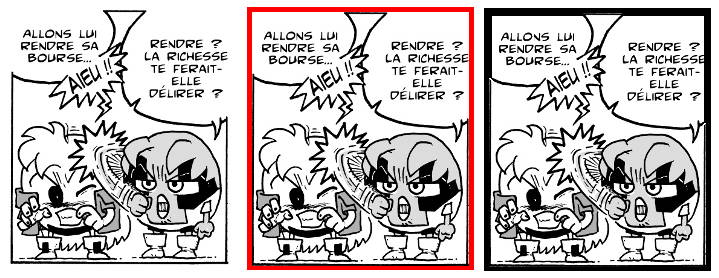
\includegraphics[trim= 0px 0px 0px 0px, clip, width=0.75\textwidth]{implicit_balloon_recovery.png}
    \caption[Implicit balloon recovering by closing open panels]{Implicit balloon recovering by closing open panels. From left to right: original panel, panel bounding box detection, panel with artificial frame from its bounding box that closes two balloons. The implicit balloons are now regular (closed).}
    \label{fig:ex:implicit_balloon_recovery_by_panel}
  \end{figure}
  %%%%%%%%%%%%%%%%%%%%%%%%%%%%%%%%%%%%%%%%%%%%%%%%%%%

However, it has two advantages in comparison with the proposed active contour based method.
First, as the connected-component is considered as balloon, when correct, the precision at the pixel level is maximal.
Second, it is faster to compute.

The presented implicit balloon extraction version of Method S highly depends on the active contour initialization success.
In this study, we relied on text detection as we assume it is the most common feature that balloons include, while past experiments have shown that its accurate detection is feasible and stable.
A side-effect of this choice is that balloons sometimes can not be detected because they contain non text information (e.g. drawings, punctuation).
% the text line detector is not always used was not able to detect balloons that contain other contents (e.g. drawings, punctuation).
%and its bounding box level may also include non-textual information (e.g. portion of the balloon contour) that alter our method. % see fig.~\ref{fig:case_of_failure}. Moreover, : text line bounding boxes removal may also remove some part of the drawing before the external energy edge detection
We believe there is room for improvement of the different energy terms we used.
For example, one could use the Gradient Vector Flow proposed by Xu~\cite{Xu1998} for the external energy, especially in the case of missing data balloon boundaries.
%We could also initialize the snake with a more balloon-like shape as the minimal ellipse including the text area for example. This would also reduce computation time.
On the other hand, the ground truth of implicit balloons is at best questionable, as the exact localization of the balloon is quite subjective.
A way to circumvent this problem could be to either define the boundary in a flexible way.
%, or match the ground truth at the pixel level.
% All the materials for reproducing and comparing the results presented in this paper are publicly available through \url{http://ebdtheque.univ-lr.fr/references}.
Our results using active contour with distance transform shows a significant improvement compared to the regular balloon extraction, thanks to the active contour theory that detect much more balloons both open or closed than connected component based methods (Table~\ref{tab:ex:balloon_localisation_comparison_results}).


%Making the edges attract the active contour from further is an essential step as we can see line (3). We gain up to {\bf X RECALL AND Y PRECISION}.
%Mono-resolution and multi-resolution shows similar recall result because the high resolution affects only the shape details, not significantly changing the location of the detection. Next section explains how to evaluate the benefits of the high-resolution detection. %However there is a slight improvement for the precision measure due to higher precision in the shape detection. {\bf ADD RESULT FIGURE?}
% Doing just the low resolution localization step, or continuing to include the high resolution fitting step does not cause any difference for Method A (3) under this evaluation scheme, as the evaluation is performed at the level of bounding boxes object overlapping.


% \modif{TODO: OTHER VERSION?}

% Our methods outperforms~\cite{Arai11} thanks to its genericity, since it can process all the image styles of the eBDtheque dataset.
% This was expected as~\cite{Arai11} was specifically developed for manga comics that have certain stylistic particularities.
% We also surpassed our previous method~\cite{rigaud2013active} because it needs text lines as input which were given in our proposed text extraction method (Section~\ref{sub:text_extraction}).
Sequential approaches such as Arai, Ho and Method S suffer from limitations of dependency between the different processing.
For instance, in Method S the performance of our text extractor was 56.01\% (Table~\ref{tab:text_results}) which was used as input for balloon extraction so the balloon extraction was inevitably affected.
Also, such approaches search for balloon inside the panel region, as a consequence, these methods can not extract balloons that overlap several panels.
This is easily handled by independent method such as Method I because it does not consider panel positions and search for balloons everywhere in the image.
The post validation by the expert system (Method K) reached the maximum precision but decreased the recall of the extraction which resulted in a drop of the overall f-measure by almost 5\% compared to Method S.
The drop in recall was due to the balloons that were correctly extracted but which contained undetected text regions.
%Nevertheless, the proposed method does not beat our previous method~\cite{rigaud2013active} that is also able to extract non closed balloons from text regions (from the ground truth here).
% This experiment was performed in 22 minutes for the whole dataset using one CPU at 2.5GHz (2.2s per balloon on average).



% \paragraph{Balloon segmentation (pixel-level)}
% \label{par:}
% Balloon localisation is enough for object detection purposes at bounding box level.


% \modif{TODO}

% Balloon segmentation is performed at the level of pixel and can reflects such level of details.
% To evaluate the segmentation level, we repeated the evaluation using a pixel level evaluation scheme.
% The results are shown in table~\ref{tab:high_res}.
% Note that for this experiment we selected three pages where ground truth and automatic text detection give the same results.

%\subsection{Balloon shape detection}
%The bounding box level ground truth we used for balloon localization evaluation is not precise enough to know if all the detail of the balloon shape have been correctly detected or not. Here we evaluate the balloon detection from a pixel level ground truth (including the tail) on few pages\footnote{Page 1 refer to ``CYB\_BUBBLEGOM\_T01\_008'', page 2 to ``6673465787\_668ec4eff4\_o'' and page 3 to ``LAMISSEB\_ETPISTAF\_013''.{\bf should I add complete ref. in ref. section instead?}} from the same dataset as section~\ref{sec:dataset} and the evaluation measures of section~\ref{sec:eval}, in order to compare the performance between mono and multi-scale detection with more accuracy (see table~\ref{tab:high_res}). Note, for this experiment we selected only pages where ground truth and automatic text detection give same results.


% Table~\ref{tab:ex:high_res} shows...



% higher score for the two-stage variant for the page 1 and 3.
% These two pages contain mainly closed balloons, we see here that the second stage improves the accuracy of the detection of closed balloons.
% In the case of implied balloon boundaries, as in page 2, the second stage is not resulting in any improvement as there is no extra local information that can assist in the fitting.

% In this case the results mainly depends  of the low resolution detection. Note, processing time was about 10 seconds for a 300DPI A4 image on a regular machine.


  %%%%%%%%%%%%%%%%%%%%%%%%%%%%%%%%%%%%%%%%%%%%%%%%%%%
%   \begin{figure}[!ht] %trim=l b r t  width=0.5\textwidth,
%     \centering
%     \includegraphics[width=170px]{fig/mono_multi_detection.png}
%     \caption{Examples of closed balloon detection. The pixel level ground truth in red, the mono-resolution detection in grey and the multi-resolution in green. {\bf ADD OPEN BALLOON EXAMPLE}}
%     \label{fig:mono_multi_detection}
%   \end{figure}
  %%%%%%%%%%%%%%%%%%%%%%%%%%%%%%%%%%%%%%%%%%%%%%%%%%%

% \subsection{Result comparison} % (fold)
% \label{sub:result_comparison}
% Here we compare the best result we obtain for each of the contribution to methods from the literature at localisation and segmentation level.
% Balloon localisation is enough for object detection purposes at bounding box level.
% As mention Section~\ref{??}, the balloon contour contains part of information that is also important to retrieve in the context of understanding comic book documents.
% Balloon segmentation is performed at the level of pixel and can reflects such level of details.


%%%%%%%%%%%%%%%%%%%%%%%%%%%%%%%%%%%%%%%%%%%%%%%%%%%
\begin{figure}[!ht] %trim=l b r t  width=0.5\textwidth, 
  \centering
  \subfloat[Arai's method]{\label{fig:ex:balloon_arai_extraction_detail}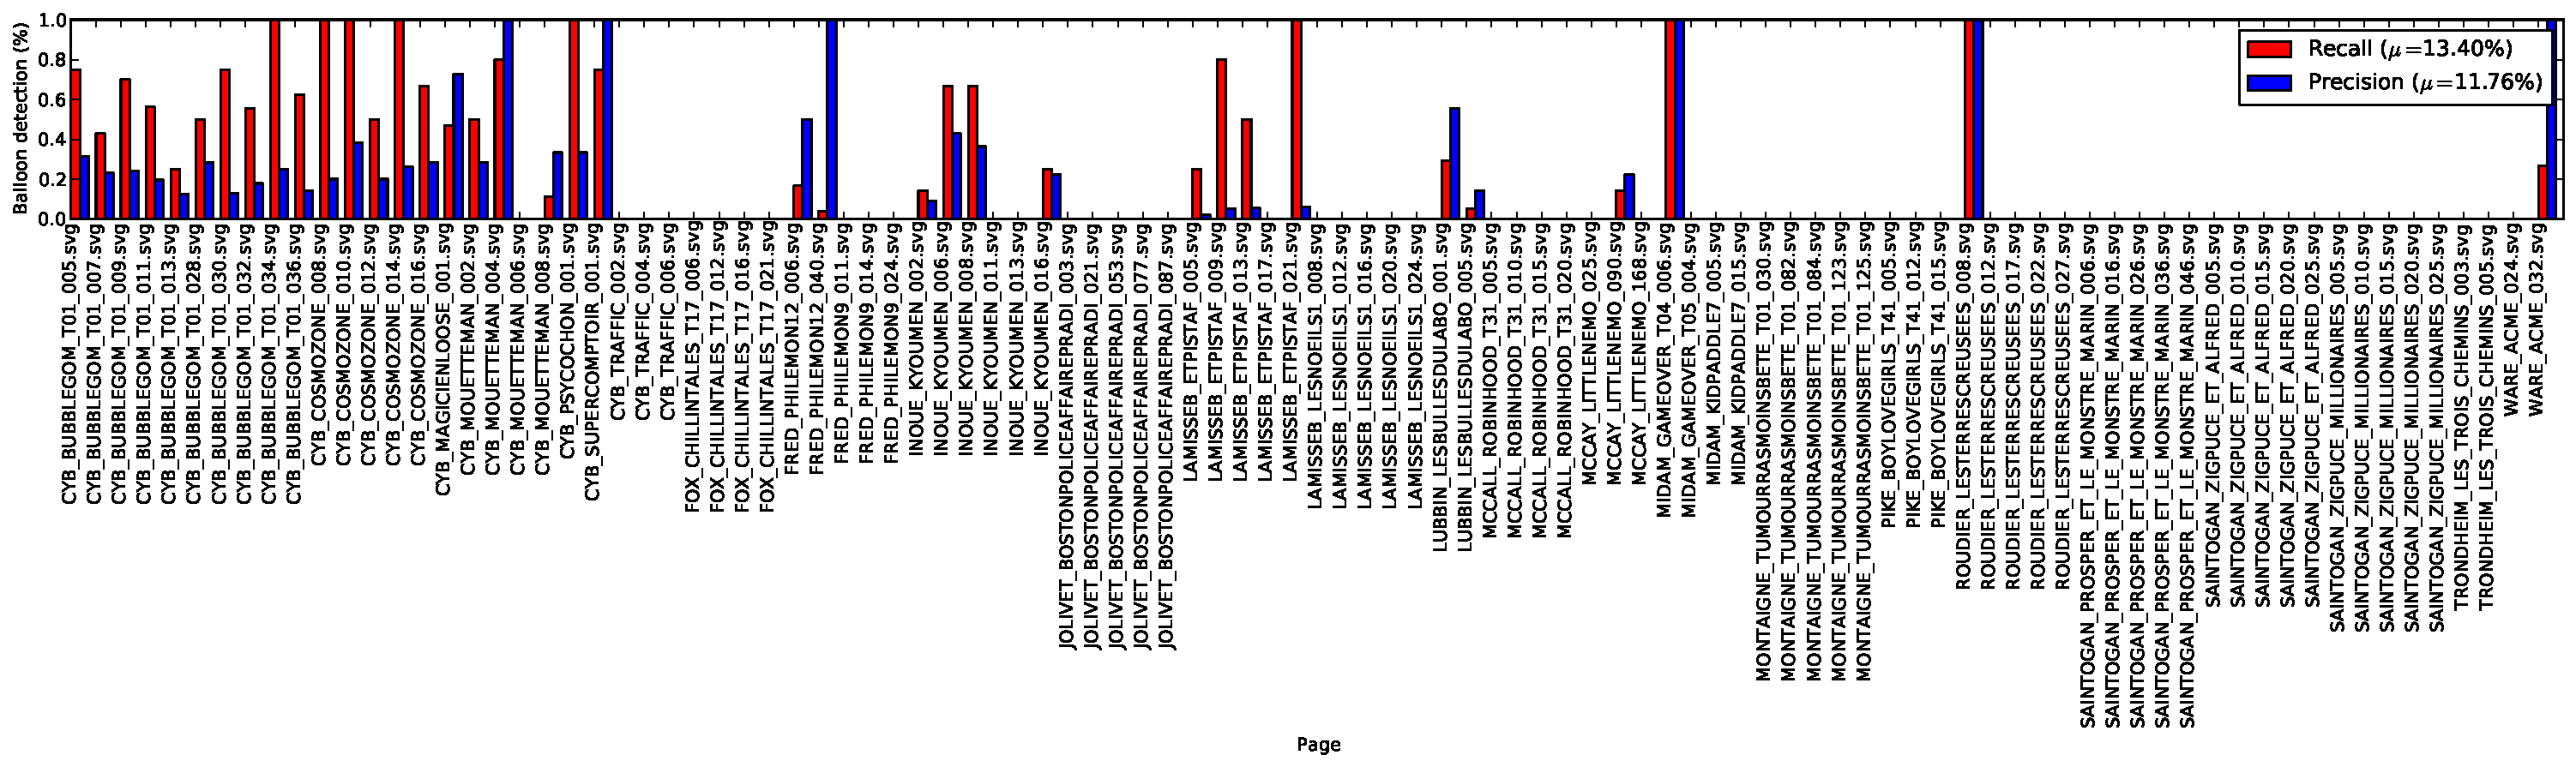
\includegraphics[trim= 0mm 108mm 0mm 0mm, clip, width=\textwidth]{2014-07-21_svg_Arai2011_Balloon.pdf}}
  \\
  \subfloat[Ho's method]{\label{fig:ex:balloon_ho_extraction_detail}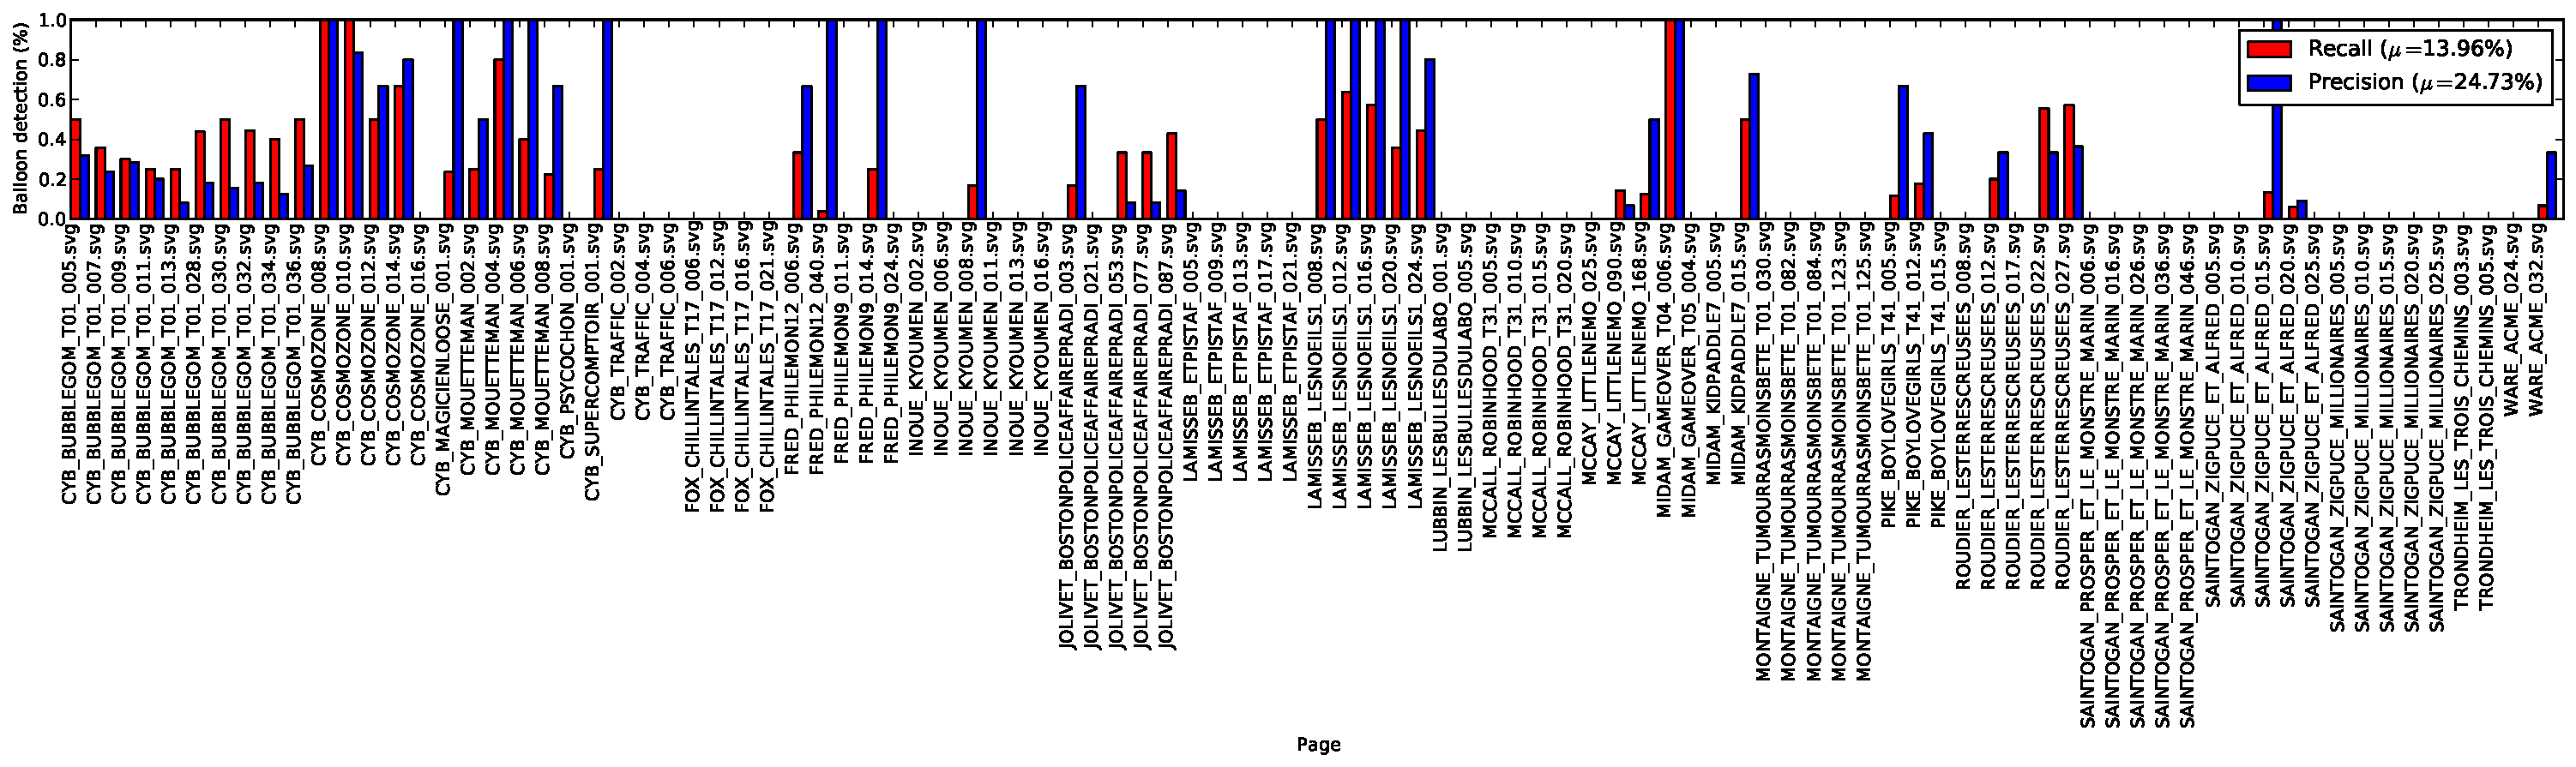
\includegraphics[trim= 0mm 108mm 0mm 0mm, clip, width=\textwidth]{2014-07-22_svg_Ho2012_Balloon.pdf}}
  \\
  \subfloat[Method S (regular)]{\label{fig:ex:closed_balloon_methodA_extraction_detail}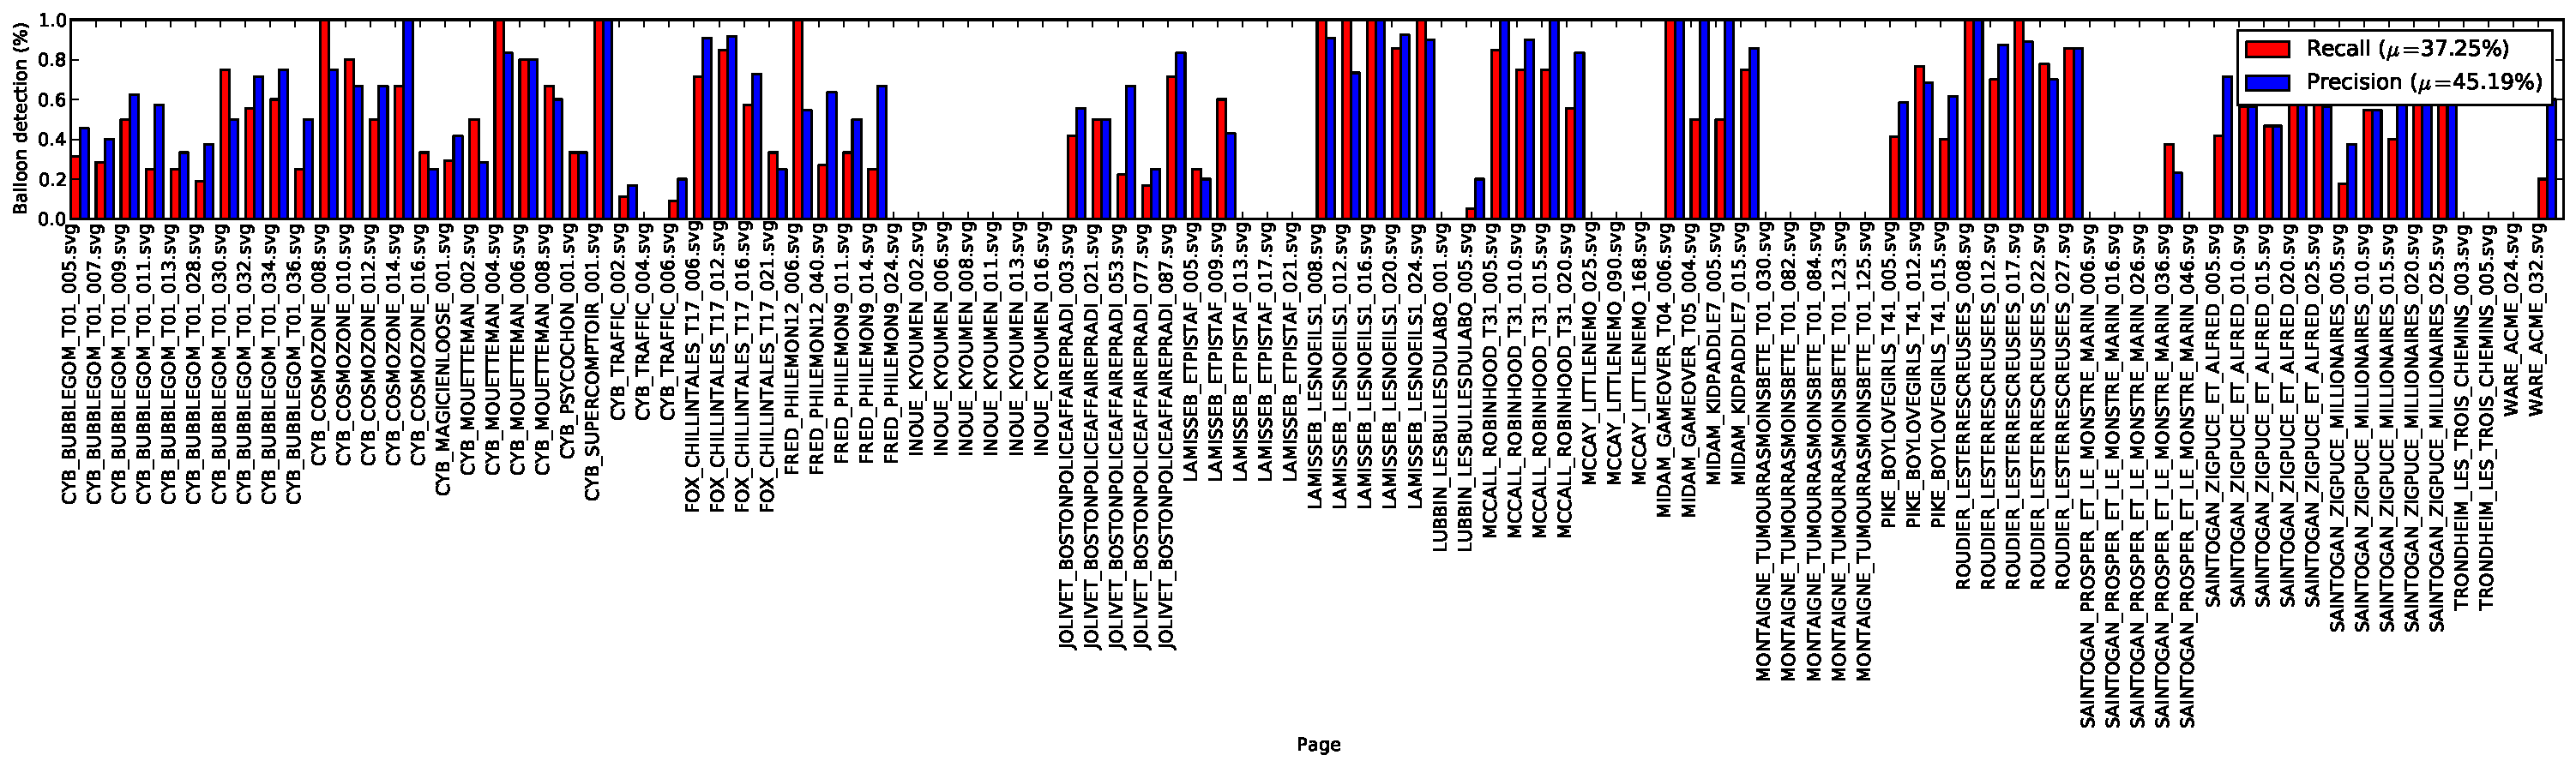
\includegraphics[trim= 0mm 108mm 0mm 0mm, clip, width=\textwidth]{2014-07-26_svg_closed_thesis_method_A_Balloon.pdf}}
  \\
  \subfloat[Method S (implicit)]{\label{fig:ex:implicit_balloon_methodA_extraction_detail}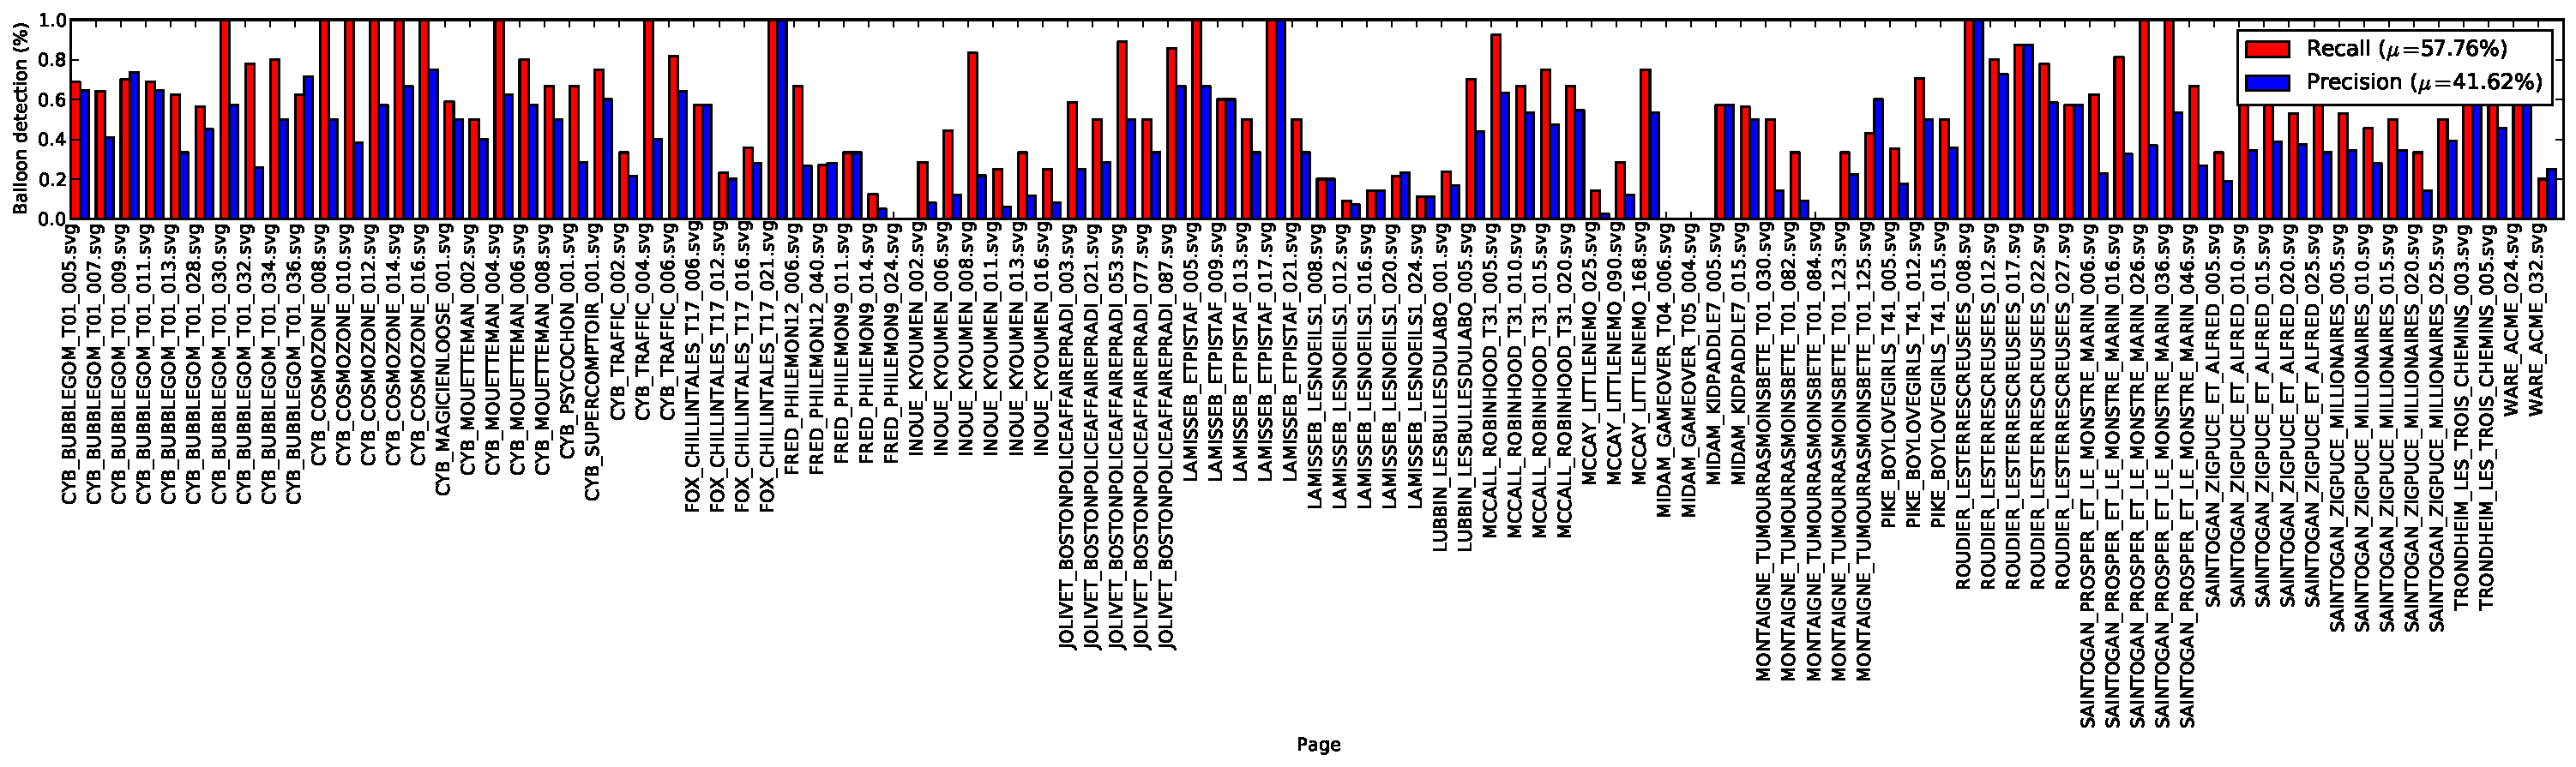
\includegraphics[trim= 0mm 108mm 0mm 0mm, clip, width=\textwidth]{2014-07-22_svg_implicit_ICDAR_Balloon_object_level.pdf}}
  \\
  \subfloat[Method I]{\label{fig:ex:balloon_methodB_extraction_detail}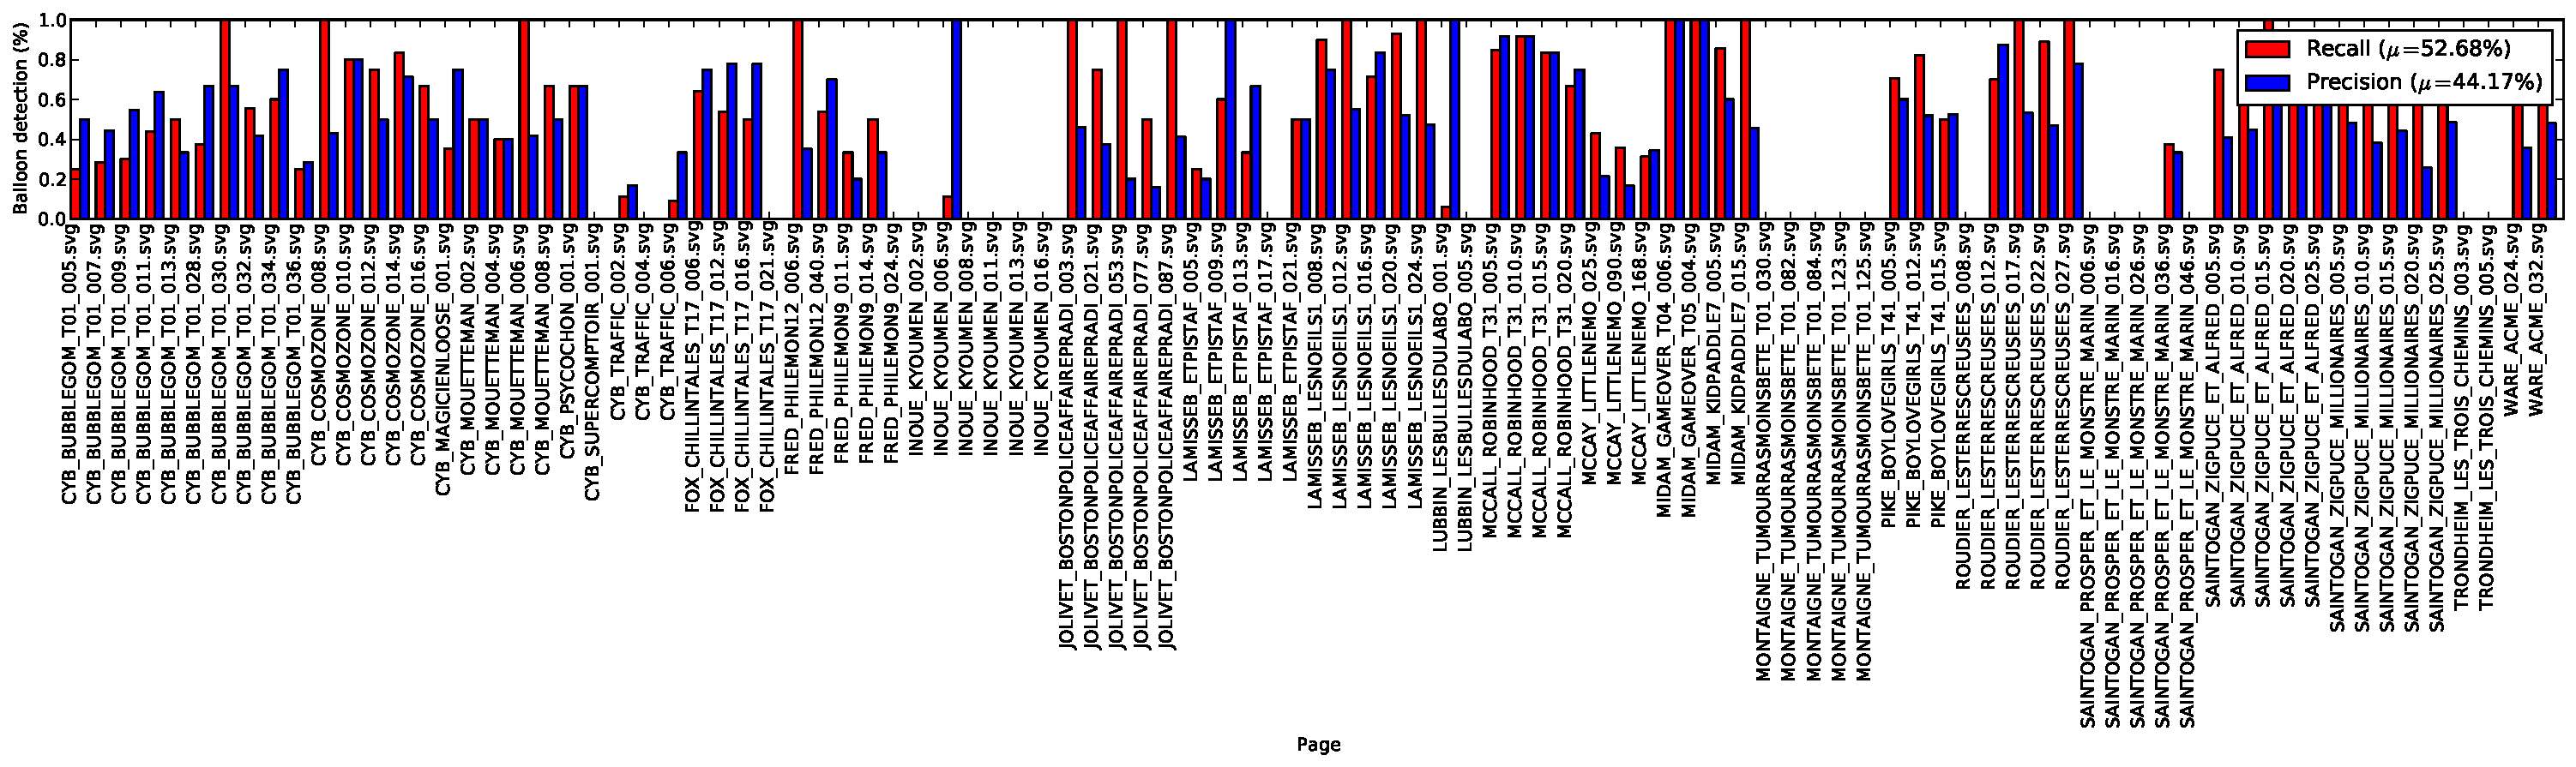
\includegraphics[trim= 0mm 108mm 0mm 0mm, clip, width=\textwidth]{2014-07-21_svg_closed_IJDAR_method_B_Balloon.pdf}}
  \\
  \subfloat[Method K]{\label{fig:ex:balloon_methodC_extraction_detail}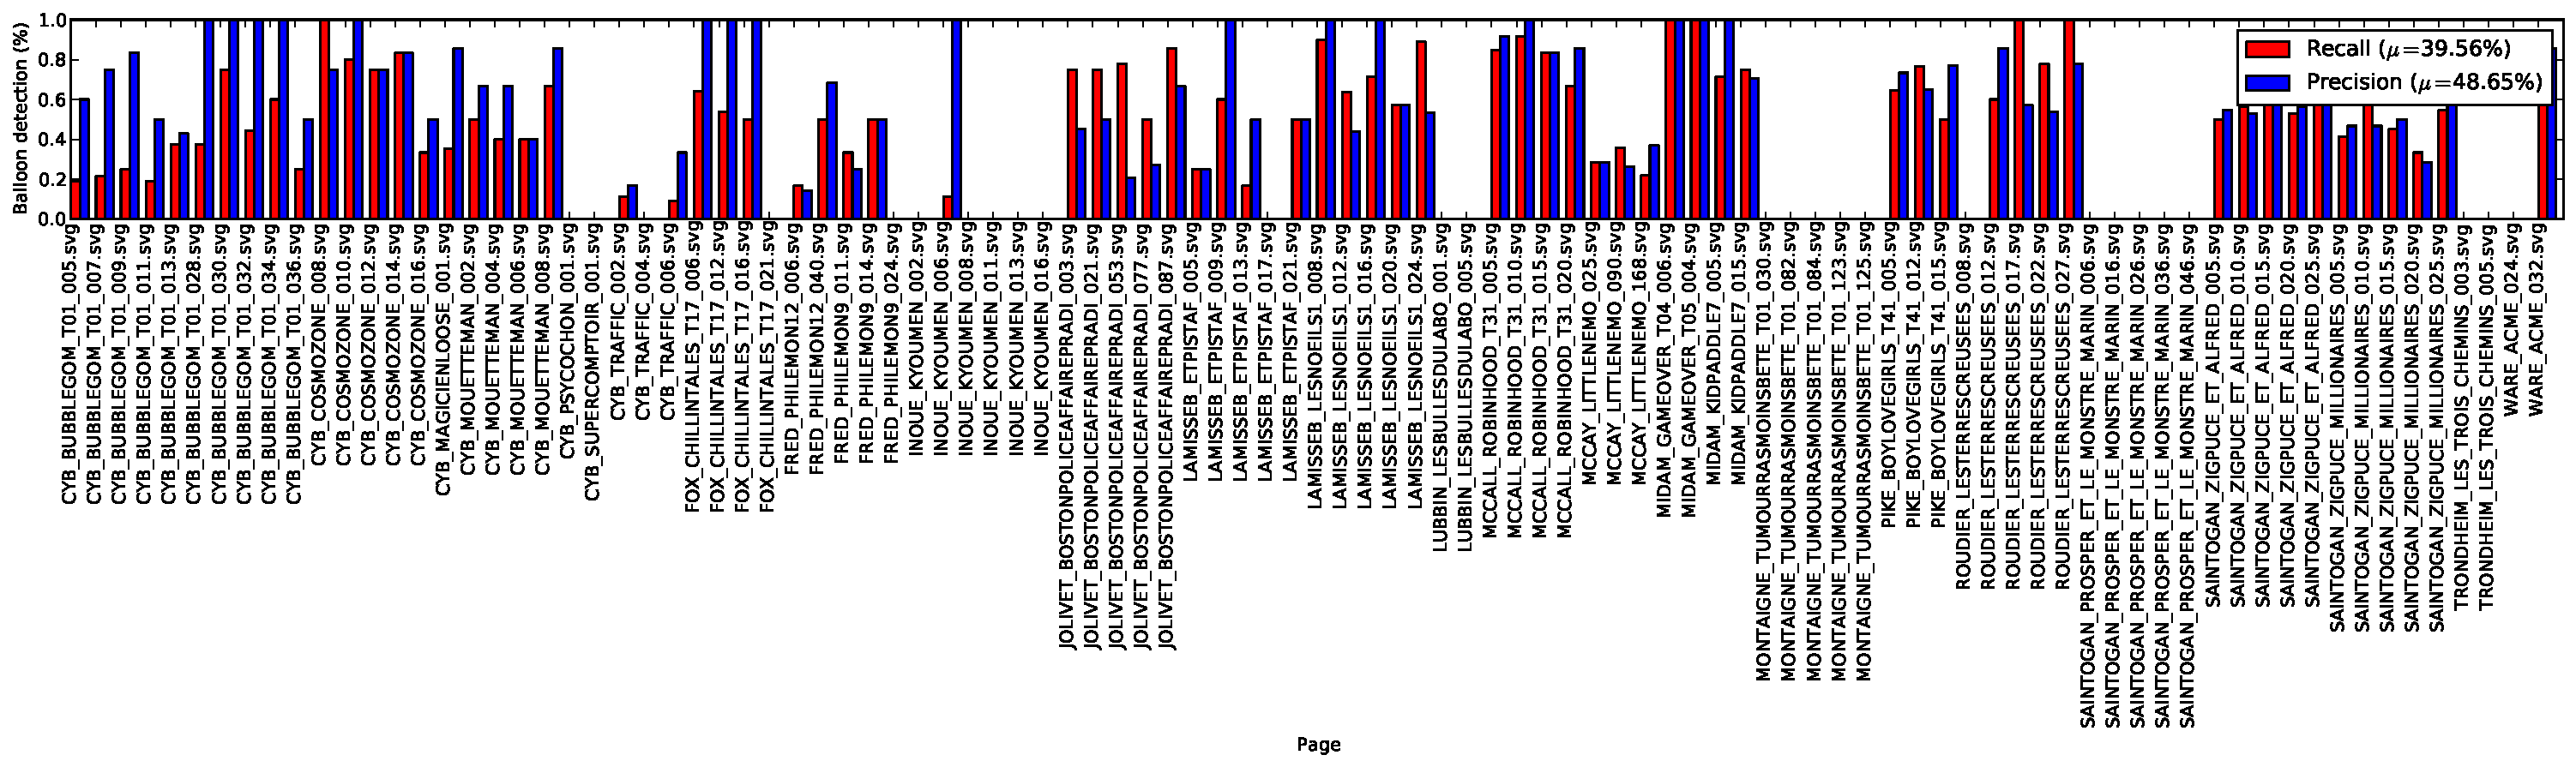
\includegraphics[trim= 0mm 0mm 0mm 0mm, clip, width=\textwidth]{2014-09-04_cleaned_validated_from_method_B_for_panel_text_balloon_and_method_A_for_character_Balloon_object.pdf}}

  \caption[Balloon extraction score details at object level for each image of the eBDtheque dataset]{Balloon extraction score details at object level for each image of the eBDtheque dataset (Appendix~\ref{app:dataset}).}
    \label{fig:ex:balloon_detection_result_details}
\end{figure}
%%%%%%%%%%%%%%%%%%%%%%%%%%%%%%%%%%%%%%%%%%%%%%%%%%%

% subsection result_comparison (end)


\section{Balloon classification} % (fold)
\label{sub:ex:balloon_classification}
From our knowledge, this is the first work that tackles speech balloon classification.
We analyse the effects of the two features and the prior knowledge we presented in Section~\ref{sub:in:balloon_classification}.
 % using  using the pixel-level balloon segmentation from the eBDtheque ground truth.
% and from the best automatic segmentation of regular balloon from the independent approach (Method I).
We evaluate the proposed method using a subset of 914 balloons from the 1091 balloons present in the original eBDtheque ground truth (only ``smooth'', ``wavy'' and ``spiky'' balloons).
The repartition of the balloon types is 87.96\%, 8.75\% and 3.29\% of type ``smooth'', ``wavy'' and ``spiky'' respectively.
This unbalanced repartition reflects the usual speech balloon types repartition in comics.

In the shape/contour separation process (Section~\ref{sec:contour_detection}), we first cast the original signal $o$ into 360 values and then smooth it in order to approximate the shape signal $s$.
The shape signal is also composed by 360 values where each of them corresponds to the local mean in a window of size $M$ from the original signal (Equation~\ref{eq:ex:shape_approximation}).
Note that in order to avoid side effects we copy $M/2$ values from the opposite side when needed (wrapping).
A validation of parameter $M$ have been performed and its best value was $M=7$.

\begin{equation}
  \label{eq:ex:shape_approximation}
  s(i) = 1/M \sum_{j=i-M/2}^{i+M/2} o(i)
\end{equation}

 %smoothing process divides the 360 values into $M$ segments and compute the mean of size $360/M$ according to 
 % A validation of parameter $M$ have been performed and its best value was $M=7$.
 % (Table~\ref{tab:validation_parameter_m}).
%In other words, we split the balloon contour into 20 sectors of 18 degrees each.
%which correspond to 5.5\% of 360 values 
% This parameter can be adjusted according the contour descriptor type.

  %%%%%%%%%%%%%%%%%%%%%%%%%%%%%%%%%%%%%%%%%%%%%%%%%%%
%   \begin{table}[ht]
%     \normalsize
% \renewcommand{\arraystretch}{1.2}

%     \centering
%     \caption{Validation of parameter $M$ for $D=(f_1,f_2)$ scenario \modif{TODO: update with new training set?}.}
%     \begin{tabular}{c|c|c|c|c|c|}
%   \cline{2-6}
%     & \multicolumn{5}{|c|}{Accuracy per class (\%)} \\
%   \cline{2-6}
%     & Smooth & Wavy & spiky & Avg & Global \\
%   \hline
%   \multicolumn{1}{ |c| }{$M=10$}& 80.63   & \textbf{70.58} & 58.80 & 70.00 & 75.8 \\
%   \hline
%   \multicolumn{1}{ |c| }{$M=20$}& \textbf{89.30}  & 69.1  & 86.20 & \textbf{81.53} & \textbf{85.2} \\
%   \hline
%   \multicolumn{1}{ |c| }{$M=30$}& 88.53 & 67.64 & \textbf{86.25}  & 80.81 & 84.4 \\
%   %\hline
%   \hline
%   \multicolumn{1}{ |c| }{$M=40$}& 87.35 & 61.76 & 82.35 & 77.15 & 81.99 \\
%   %\hline
%   \hline
%   \multicolumn{1}{ |c| }{$M=50$}& 79.05 & 63.23 & 80.39 & 74.22 & 76.34 \\
%   %\hline
%   \hline
% %       Proposed multi scale & ???  &???  & ???   & ???       \\
% %   \hline
%         \end{tabular}
%     \label{tab:validation_parameter_m}
%   \end{table}%
  %%%%%%%%%%%%%%%%%%%%%%%%%%%%%%%%%%%%%%%%%%%%%%%%%%%


We evaluated our method based on a one-versus-all scenario.
Classification results are presented in Table~\ref{tab:ex:desc_test_balloon_classification} for different descriptors.
First we show the effect of the two features $f_1$ and $f_2$ separately without \emph{a priori} information $P(l_1)=P(l_2)=P(l_3)$ and then using the prior probabilities about the classes repartition from the eBDtheque dataset $P(l_1)=0.88, P(l_2)= 0.09$ and $P(l_3)=0.03$.
We detailed our best results for balloon contour extraction (for $D=(f_1, f_2)$) in the confusion matrix Table~\ref{tab:ex:confusion_matrix_balloon_classification}.

As mentioned Section~\ref{sub:in:balloon_classification}, the region of the tail may influence balloon classification.
 % Note that we also show the results when we automatically remove the tail region from its automatic detection (Section~\ref{sec:se:from_balloon_to_tail}).
In order to measure this influence, we remove the tail by ignoring the points of the contour that are between the two points defined as tail origin (Section~\ref{sec:se:from_balloon_to_tail}), see Figure~\ref{fig:ex:tail_removal}.
Note that this process relies on the tail detection performance (Section~\ref{sec:tail_detection_evaluation}).

%   %%%%%%%%%%%%%%%%%%%%%%%%%%%%%%%%%%%%%%%%%%%%%%%%%%%
   \begin{figure}[!ht]  %trim=l b r t  width=0.5\textwidth,
     \centering
    \includegraphics[trim= 0px 0px 0px 0px, clip, width=0.75\textwidth]{tail_removal.png}
    \caption[Tail removal for balloon classification]{Two examples of tail removal for balloon classification. From left to right, original contour detection in red, corresponding mask and partial contour removal between the two green points that represent the tail origin. The final contour is represented in purple in the right figures.}
    \label{fig:ex:tail_removal}
   \end{figure}
%   %%%%%%%%%%%%%%%%%%%%%%%%%%%%%%%%%%%%%%%%%%%%%%%%%%%


    %%%%%%%%%%%%%%%%%%%%%%%%%%%%%%%%%%%%%%%%%%%%%%%%%%%
  \begin{table}[ht]
    \normalsize
    \renewcommand{\arraystretch}{1.2}

    \centering
    \caption[Classification result accuracy for different descriptor configuration]{Classification result accuracy for different descriptor configuration. The global accuracy represents the number of good classification divided by the number of elements to classify independently from the class.
}
    \begin{tabular}{c|c|c|c|c|c|}
  \cline{2-6}
    & \multicolumn{5}{|c|}{Accuracy per class (\%)} \\
  \cline{2-6}
    & Smooth & Wavy & Spiky & Average & Global \\
  \hline
  \multicolumn{1}{ |c| }{ $D=(f_1)$ } & 22.51 & 68.75 & 33.33  & 41.53 & 26.91  \\
  \hline
  \multicolumn{1}{ |c| }{ $D=(f_2)$ } & 79.73 & 36.25 & 70.00 & 61.99 & 75.60 \\
  \hline
  \multicolumn{1}{ |c| }{$D=(f_1, f_2)$ } & 76.62 & \textbf{60.00} & \textbf{73.34} & \textbf{64.33} & 75.05\\
  %\hline
  \hline
  \multicolumn{1}{ |c| }{$D=(f_1, f_2)$ + $priors$}   & \textbf{98.26} & 11.25 & 63.34 & 57.62 & \textbf{89.50}  \\
  %\hline
  \hline
%       Proposed multi scale & ???  &???  & ???   & ???       \\
%   \hline
        \end{tabular}
    \label{tab:ex:desc_test_balloon_classification}
  \end{table}%
    %%%%%%%%%%%%%%%%%%%%%%%%%%%%%%%%%%%%%%%%%%%%%%%%%%%


    %%%%%%%%%%%%%%%%%%%%%%%%%%%%%%%%%%%%%%%%%%%%%%%%%%%
  \begin{table}[ht]
    \normalsize
    \renewcommand{\arraystretch}{1.2}

    \centering
    \caption{Confusion matrix for smooth (S), wavy (W) and spiky (Z) balloon contour classification results with $D=(f_1, f_2)$.}
    \begin{tabular}{cc|c|c|c|c|c|c|}
  \cline{3-8}
   & & \multicolumn{3}{|c|}{Ground truth}  & \multicolumn{3}{|c|}{Ground truth no tail}  \\
  \cline{3-8}
   & & S & W  & Z & S & W  & Z  \\
  \hline
  \multicolumn{1}{ |c|  }{\multirow{3}{*}{Prediction} } & S & \textbf{616} & 180 & 8 & 114 & 349 & 341   \\
  \cline{2-8}
  \multicolumn{1}{ |c  }{} & \multicolumn{1}{ |c| }{ W } & 30  & 48 & 2 & 7 & \textbf{53} & 20  \\
  \cline{2-8}
  \multicolumn{1}{ |c  }{} & \multicolumn{1}{ |c| }{ Z } & 4 & 4 & \textbf{22} & 4 & 13 & 13  \\
  % \hline
  % \multicolumn{2}{ |c|  }{TOTAL}  & 804 & 80 & 30  & 804 & 80 & 30  \\
  %\hline
  \hline
%       Proposed multi scale & ???  &???  & ???   & ???       \\
%   \hline
        \end{tabular}
    \label{tab:ex:confusion_matrix_balloon_classification}
  \end{table}%
    %%%%%%%%%%%%%%%%%%%%%%%%%%%%%%%%%%%%%%%%%%%%%%%%%%%


% An example of the Gaussian distribution parameters of the training set presented Figure~\ref{fig:ex:balloon_training_set} is given Table~\ref{tab:ex:coefficient_balloon_classification}.
% Those parameters can be used for other dataset containing similar images without needing to train the classifier again.


%   %%%%%%%%%%%%%%%%%%%%%%%%%%%%%%%%%%%%%%%%%%%%%%%%%%%
%    \begin{figure}[!ht]  %trim=l b r t  width=0.5\textwidth,
%      \centering
%     \includegraphics[trim= 0px 0px 0px 0px, clip, width=0.7\textwidth]{figure_here.png}
%     \caption[Training set for balloon contour classification]{Training set for balloon contour classification.}
%     \label{fig:ex:balloon_training_set}
%    \end{figure}
%   %%%%%%%%%%%%%%%%%%%%%%%%%%%%%%%%%%%%%%%%%%%%%%%%%%%



  %%%%%%%%%%%%%%%%%%%%%%%%%%%%%%%%%%%%%%%%%%%%%%%%%%%
%   \begin{table}[ht]
%     % \normalsize
% % \renewcommand{\arraystretch}{1.2}

%     \centering
%     \caption{Example of Gaussian distribution parameters.}
%     \begin{tabular}{|c|c|c|c|c|c|c|}
%   \hline
%     & \multicolumn{2}{|c|}{Smooth}& \multicolumn{2}{|c|}{Wavy}& \multicolumn{2}{|c|}{spiky}  \\
%   \hline
%     & $\mu$ & $\sigma$ & $\mu$ & $\sigma$ & $\mu$ & $\sigma$    \\
%   \hline
%     Feature $f_1$ & 0.019   & 0.012 & 0.042 & 0.020 & 0.148 & 0.118   \\
%   \hline
%     Feature $f_2$ & -0.004  & 0.006 & 0.007 & 0.010 & -0.017 & 0.023   \\
%   \hline
%    %\multicolumn{1}{ |c| }{ Feature 2 } &  8  & 5 & 15 & 6 & 8 & 4 \\
%   %\cline{2-5}
%   %\multicolumn{1}{ |c  }{} & \multicolumn{1}{ |c| }{\textbf{ spiky }}   & ? & ? & 12 \\
%   %\hline
%   %\hline
% %       Proposed multi scale & ???  &???  & ???   & ???       \\
% %   \hline
%         \end{tabular}
%     \label{tab:ex:coefficient_balloon_classification}
%   \end{table}%
  %%%%%%%%%%%%%%%%%%%%%%%%%%%%%%%%%%%%%%%%%%%%%%%%%%%


% \modif{TODO: Ces valeurs sont pour quels types de dessins (cf. Figure4.11). 
% ESt ce que cette méthode peut prendre en compte cette diversité de représentation.... Cette remarque est un peu provocatrice, mais on pourrait te poser la question.. 
% Puisque tu commences la section en montrant les différents styles et la complexité et tu enchaines sur une méthode... on peut donc s'attendre à une conclusion sur ce que ta méthode est capable d'apporter par rapport à toutes ces représentations.}


The different accuracy results Table~\ref{tab:ex:desc_test_balloon_classification} show that the first feature $f_1$ is more appropriate for separating ``wavy'' from the rest while the second feature $f_2$ is more efficient for ``smooth'' and ``spiky'' separation.
 % more discriminant than the first one $f_1$ and their combination does not exceed the second itself ($f_2)$.
Their combination ($f_1, f_2$) is therefore the best solution for dividing the balloons into these three classes.
Adding the prior knowledge about the testing classes repartition improves the score of the ``smooth'' class and decrease the two others.
This is due to the consideration of the probability of 88\% to be in the ``smooth'' class by the Bayesian classifier.
The confusion matrix Table~\ref{tab:ex:confusion_matrix_balloon_classification} shows good classification results for the ``spiky'' class even for cases that are quite different in terms of drawing styles (Figure~\ref{fig:good_detection_balloon_classification}).
Concerning the ``smooth'' and ``wavy'' classes, some speech balloons are very hard to classify out of context causing confusion (Figure~\ref{fig:bad_detection_balloon_classification}).
Also, the tail of the balloon creates some noise and the radius average ($\bar{o}$) we use to normalize the descriptor features may not be appropriate for elongated balloons.


  %%%%%%%%%%%%%%%%%%%%%%%%%%%%%%%%%%%%%%%%%%%%%%%%%%
  \begin{figure}[h]  %trim=l b r t  width=0.5\textwidth,
    \centering
    \includegraphics[trim = 0mm 0mm 0mm 0mm, clip, width=300px]{good_detection.png}
    \caption{Correct classification examples for ``spiky'' (top) and ``smooth'' classes (bottom).}
    \label{fig:good_detection_balloon_classification}
  \end{figure}
  %%%%%%%%%%%%%%%%%%%%%%%%%%%%%%%%%%%%%%%%%%%%%%%%%%


  %%%%%%%%%%%%%%%%%%%%%%%%%%%%%%%%%%%%%%%%%%%%%%%%%%
  \begin{figure}[h]  %trim=l b r t  width=0.5\textwidth,
    \centering
    \includegraphics[trim = 0mm 0mm 0mm 0mm, clip, width=300px]{bad_detection.png}
    \includegraphics[trim = 0mm 0mm 0mm 0mm, clip, width=300px]{wavy_instead_smooth.png}
    \caption{Wrong classification examples which have been classified as ``smooth'' instead of  ``wavy'' in the first row and ``wavy'' instead of  ``smooth'' in the second row.}
    \label{fig:bad_detection_balloon_classification}
  \end{figure}
  %%%%%%%%%%%%%%%%%%%%%%%%%%%%%%%%%%%%%%%%%%%%%%%%%%


\subsection{Results analysis} % (fold)
\label{par:balloon_classification_analysis}

As mentioned in Section~\ref{sub:in:balloon_classification}, the balloon contour contains part of information that is also important to retrieve in the context of understanding comic book documents (e.g. tail, tone information).
In this context, the location of the balloon is not enough sufficient.
 % in our case because later we will also consider tail detection based on balloon contour analysis.
Such analysis requires a finer extraction of the balloon contour at pixel level (Table~\ref{tab:ex:balloon_localisation_comparison_results}).

The proposed method covers the comics balloon classification in general, except for open balloons.
However, in this particular case, we can probably use extra features (e.g. tail type recognition, language analysis) to get more information about the text tone.
Also, other distortion measures have to be investigated, especially for ``wavy'' contours that are the most difficult contour to classify using the proposed method.
%In this study, the proposed descriptor we proposed is not sensitive enough to properly classify the ``wavy'' nor the definition of what is a ``wavy'' contour as to be revised.
Concerning the tail region, its removal is not has significant as expected, it only improves the accuracy of ``wavy'' balloon classification (Table~\ref{tab:ex:confusion_matrix_balloon_classification}).
This is probably due to the reduction of the number of points of the balloon contour to 360 values which also reduce the impact of the tail region.

% paragraph balloon_classification_analysis (end)

% subsection balloon_classification (end)



\section{Tail detection evaluation} % (fold)
\label{sec:tail_detection_evaluation}

% \subsection{Experimental settings} % (fold)
% \label{sub:experimental_settings}

In this section we evaluate the tail extraction method on the 1091 balloons of the eBDtheque dataset~\cite{Guerin2013} from three balloon extraction methods, one manual and two automatic extractions.
The automatic extraction methods are the two best methods for regular (Method I) and implicit (Method S) from the summary given in Table~\ref{tab:ex:balloon_localisation_comparison_results}.
The manual method is the balloon contours from the eBDtheque dataset.
The comparison of the three balloon extraction method will highlight the part of error which comes from the balloon extraction and the proper tail extraction method's error when there is not possible error from the balloon extraction.
As introduced in Section~\ref{sub:ex:tail_detection_metric}, we use two accuracy metrics, one for the predicted position of the tail tip $A_{tailTip}$ and the other one for the tail direction $A_{tailDir}$
 (Table~\ref{tab:ex:tail_evaluation}).

%and from the regular and implicit balloon extraction methods presented Section~\ref{sec:se:from_text_to_balloon} as their are the previous steps in the sequential approach (Table~\ref{tab:ex:tail_evaluation}).


% \subsection{Result analysis} % (fold)
% \label{sub:result_analysis}

    %%%%%%%%%%%%%%%%%%%%%%%%%%%%%%%%%%%%%%%%%%%%%%%%%%%
  \begin{table}[h]
    % \normalsize
%\renewcommand{\arraystretch}{1.2}

    \centering
    \caption{Tail tip position ($A_{tailTip}$) and tail direction ($A_{tailDir}$) extraction results from automatic and manual balloon contour extractions.}
    \begin{tabular}{|c|c|c|}
          % \hline
          %   & \multicolumn{2}{|c|}{Character 1}   & \multicolumn{2}{|c|}{Character 2}   \\
          \hline
          Balloon extraction method&  $A_{tailTip}$ (\%)  & $A_{tailDir}$ (\%)    \\
          \hline
          Ground truth        & \textbf{96.61}    & \textbf{80.40}     \\
          \hline
          Automatic (regular balloons)    & 55.77    & 27.59     \\
          \hline
          Automatic (regular + implicit balloons)    & 64.34    & 20.21     \\
          \hline
          % Proposed + validation   & \modif{??}       & \modif{??}    & \modif{??}    \\
          % \hline
           % TOTAL   & 93.4    & 92.8          \\
          % \hline
        %       Proposed multi scale & ???  &???  & ???   & ???       \\
        %   \hline
        \end{tabular}
    \label{tab:ex:tail_evaluation}
  \end{table}%
    %%%%%%%%%%%%%%%%%%%%%%%%%%%%%%%%%%%%%%%%%%%%%%%%%%%


% \begin{itemize}
%   \item balloon segmentation must be done on the exterior edge of the balloon contour. It has an impact on the tail direction computation. 
%   \item issue when the tail does not correspond to any vertex of the convex hull (assumption in 3.4)
% \end{itemize}
% subsection result_analysis (end)

\subsection{Result analysis} % (fold)
\label{sub:ex:result_analysis_tail_evaluation}

% subsection result_analysis (end)

The proposed method is very good at locating the tail tip when it existed and also at giving a confidence value equal to zero when the balloon has no tail.
The few mistakes concerning the tail tip position detection is due to very small tails or when there are variations along the contour but no tail to detect which confuse the vertex selection process.
The tail direction is sensitive to the quality of the pixel-level balloon contour extraction in the area of the tail tip.
Sometimes, the inside balloon region extraction is not sufficient to retrieve the tail direction, the balloon border has also to be considered.
For instance, in Figure~\ref{fig:ex:tail_extraction_mistake_errors}, the tail positions are represented by a green line on the balloon contour and tail directions are written in blue (from the eight cardinal coordinates).
Left hand side balloons have not been detected without tail because of the contour variations, a tail have been mistakenly predicted.
For the right hand side balloons, the tail tip position have been correctly predicted but not the tail direction because of the change of direction of the last segment.
The direction have been predicted according the white balloon background region and not from the balloon boundary that indicates a different direction (NE and SE instead of S and E).

The tail tip position and tail direction highly rely on the performance of the balloon contour extraction.
They are satisfactory when balloon contours are perfectly extracted (manual in Table~\ref{tab:ex:tail_evaluation}) but decreases quickly according to the automatic balloon extractor method performance.
The importance of a precise pixel-level segmentation in the region of the tail tip is illustrated by the difference of 7.38\% for $A_{tailDir}$ between the regular and implicit automatic methods due to the lack of precision of the active contour extraction method.


  %%%%%%%%%%%%%%%%%%%%%%%%%%%%%%%%%%%%%%%%%%%%%%%%%%%
  \begin{figure}[h]  %trim=l b r t  width=0.5\textwidth,
    \centering
    \includegraphics[trim= 0px 0px 0px 0px, clip, width=0.75\textwidth]{tail_extraction_errors.png}
    \caption[Examples of difficult balloons for tail tip position and tail direction extractions]{Examples of difficult balloons for tail tip position (left column) and tail direction (right column) extractions.}
    \label{fig:ex:tail_extraction_mistake_errors}
  \end{figure}
  %%%%%%%%%%%%%%%%%%%%%%%%%%%%%%%%%%%%%%%%%%%%%%%%%%%

% paragraph tail_detection (end)



% subsection sequential_information_extraction_evaluation (end)


\section{Comic character extraction evaluation} % (fold)
\label{sec:comic_character_extraction_evaluation}
We evaluated the detection of comic characters on the 1597 characters of the eBDtheque dataset.
In the eBDtheque ground truth, only 829 (52\%) of the character instances are speaking (and 48\% are not).
Therefore, we do not expect to reach 100\% recall and precision with the Method S and K because they are only able to extract speaking characters.
The independent Method I is potentially able to retrieve all the character instances of colourful comics, given one example for each of them.
This limitation requires a lot a manual work thus we selected only 22 different characters which represent 352 instances in total.

% \subsubsection{Sequential approach} % (fold)
% \label{sub:sequential_approach}

% subsection sequential_approach (end)
Similarly to the other object extraction methods, the overlapping ratio between a predicted character region and a region from the ground truth should be above 50\% ($a_0>0.5$) for the predicted region to be considered as valid (Section~\ref{sub:ex:object_localisation_metric}).
This ratio can be relaxed according to the application (e.g. face only, full body, cropped body).
An example of the impact of this ratio on validation and rejection of predicted regions is shown on Figure~\ref{fig:ex:characters_overlap_ratio}.
For instance, the predictions that are presented in the panels of Figure~\ref{fig:ex:characters_overlap_ratio} could be accepted if the target was to roughly detect comic character locations.
In this case, all the predicted regions would have been accepted as correct with a validation criterion set to $a_0>0.1$.


%, at level of object using equation
%  with $th_0=0.2$.
%Here we set $th_0=0.2$ (not 0.5) in order to accept prediction of the comic character location even if they are only partial, see figure~\ref{fig:ex:characters_overlap_ratio}.
  %to equation~\ref{eq:recall}.
%In the eBDtheque dataset~\cite{Guerin2013}, ??\% of the characters are in an image where there are no  


    %%%%%%%%%%%%%%%%%%%%%%%%%%%%%%%%%%%%%%%%%%%%%%%%%%%%%%%
    \begin{figure}[ht]%trim=l b r t  width=0.5\textwidth,  
      \centering
      \includegraphics[trim= 0mm 0mm 190mm 0mm, clip, width=0.41\textwidth]{characters_overlap_ratio.png}
      % \hspace{1em}
      \includegraphics[trim= 0mm 0mm 0mm 0mm, clip, width=0.49\textwidth]{overlap_ratio_evolution.pdf}
      \caption[Example of comic character region prediction]{Example of predicted region considered as true (green) or false (red) positives according to the validation criteria $a_0>0.5$ (dashed lines in the right hand side figure). Thin grey rectangles are the ground truth regions and the red numbers in the top left corner of each ground truth region is the value of the overlapping ratio $a_0$. Image credits:~\cite{Magicien11}.}
      \label{fig:ex:characters_overlap_ratio}
    \end{figure}  
    %%%%%%%%%%%%%%%%%%%%%%%%%%%%%%%%%%%%%%%%%%%%%%%%%%%%%%%

% \subsection{Experimental settings} % (fold)
% \label{sub:experimental_settings}

\subsection{Sequential approach} % (fold)
% \label{sub:method_a}

Method S is a sequential approach that computes a region of interest for comic characters from the tail tip position and tail direction inside a panel region (Section~\ref{sec:se:tail_to_character}).
Its position is shifted in the region of the tail tip according to the tail direction which is quantized in eight cones of $\pi/4$ radius.
We evaluated the performance of this method given the input information of panel, balloon and tail from the eBDtheque ground truth and from the best automatic extraction methods from Table~\ref{tab:panel_extraction_comparision_results},~\ref{tab:ex:balloon_localisation_comparison_results} and~\ref{tab:ex:tail_evaluation} respectively (Figure~\ref{fig:ex:character_method_A_GT_extraction_detail} and~\ref{fig:ex:character_method_A_auto_extraction_detail}).
Also, two set of images have been tested, one including all the comic character instances of the eBDtheque dataset and an other one with only the speaking characters as this method is only able to predict speaking character location from the tail direction (Table~\ref{tab:ex:character_localisation_result_summary}).
% The score of this method was in average for recall and precision of 15.59\% and 83.81% (Figure 6.12c).

 
% Table~\ref{tab:ex:character_localisation_result_summary} shows the results we obtained and the detail are given for each image of the dataset in Figure~\ref{fig:ex:character_methodA_extraction_detail}.


%%%%%%%%%%%%%%%%%%%%%%%%%%%%%%%%%%%%%%%%%%%%%%%%%%
% \begin{table}[ht]
%   % \normalsize
% % \renewcommand{\arraystretch}{1.3}
% % \extrarowheight as needed to properly center the text within the cells
%   \centering
%   \caption{Comic character localisation result for method A from manual and automatic panel and balloon element extractions.}
%   \begin{tabular}{|c|c|c|c|}
%   % \hline
%   % Previous extractions  & \multicolumn{3}{|c|}{Performance}   \\
%   \hline
%   Previous extractions  &  $ R$ (\%)  & $P$ (\%)& $F$ (\%)   \\
%   \hline
%   Ground truth &  15.59    &  23.18   &  18.64   \\
%   \hline
%   Automatic &  6.84    &   12.13     &   8.75  \\
%   \hline
%   \end{tabular}
%       \label{tab:ex:character_localisation_result_summary}
% \end{table}%
    %%%%%%%%%%%%%%%%%%%%%%%%%%%%%%%%%%%%%%%%%%%%%%%%%%%



%%%%%%%%%%%%%%%%%%%%%%%%%%%%%%%%%%%%%%%%%%%%%%%%%%%
\begin{figure}[!ht] %trim=l b r t  width=0.5\textwidth, 
  \centering
  \subfloat[Method S (ground truth)]{\label{fig:ex:character_method_A_GT_extraction_detail}\includegraphics[trim= 0mm 108mm 0mm 0mm, clip, width=\textwidth]{2014-08-28_svg_method_A_from_GT_panel_balloon_Object.pdf}}
  \\
  \subfloat[Method S (automatic)]{\label{fig:ex:character_method_A_auto_extraction_detail}\includegraphics[trim= 0mm 0mm 0mm 0mm, clip, width=\textwidth]{2014-08-28_svg_method_A_from_method_B_panel_and_balloon_Object.pdf}}
  \\
  % \subfloat[Method A (regular)]{\label{fig:ex:balloon_methodA_extraction_detail}\includegraphics[trim= 0mm 108mm 0mm 0mm, clip, width=\textwidth]{2014-07-26_svg_closed_thesis_method_A_Balloon.pdf}}
  % \\
  % \subfloat[Method A (implicit)]{\label{fig:ex:balloon_methodA_extraction_detail}\includegraphics[trim= 0mm 108mm 0mm 0mm, clip, width=\textwidth]{2014-07-22_svg_implicit_ICDAR_Balloon_object_level.pdf}}
  % \\
  % \subfloat[Method B]{\label{fig:ex:balloon_methodB_extraction_detail}\includegraphics[trim= 0mm 108mm 0mm 0mm, clip, width=\textwidth]{2014-07-21_svg_closed_IJDAR_method_B_Balloon.pdf}}
  % \\
  % \subfloat[Method C \modif{TODO: update}]{\label{fig:ex:balloon_methodC_extraction_detail}\includegraphics[trim= 0mm 0mm 0mm 0mm, clip, width=\textwidth]{2014-08-28_svg_method_A_from_method_B_panel_and_balloon_Object.pdf}}

  \caption[Character extraction score details at object level for each image of the eBDtheque dataset]{Character extraction score details at object level for each image of the eBDtheque dataset for speaking and non speaking characters (Appendix~\ref{app:dataset}).}
    \label{fig:ex:character_methodA_extraction_detail}
\end{figure}
%%%%%%%%%%%%%%%%%%%%%%%%%%%%%%%%%%%%%%%%%%%%%%%%%%%

%%%%%%%%%%%%%%%%%%%%%%%%%%%%%%%%%%%%%%%%%%%%%%%%%%%%%%
% \begin{figure}[!h]
%  \includegraphics[width=\textwidth,height=4cm]{Panel_object_proposed.pdf}
%  \caption{Character extraction score details for each image of the eBDtheque dataset \modif{TODO: update}.
%  }
%  \label{fig:ex:character_methodA_extraction_detail}
% \end{figure}
%%%%%%%%%%%%%%%%%%%%%%%%%%%%%%%%%%%%%%%%%%%%%%%%%%%%%%

% subsection method_a (end)

\subsection{Independent approach} % (fold)
\label{sub:ex:character_extraction_method_b}

Method I consists in an independent comic character instance spotting given an example.
To perform this experiments, we asked the users to manually highlight the object position as described in Section~\ref{sec:in:input_query}.
The selection usually includes hair, head and top body colours because lower body parts are often hidden by the frame border or the posture. 
From the user pixel selection, we computed the bounding box to show that the system does not need a precise object colour selection. 
% We reduced the number of colour to a \modif{standard web palette $P_c$ of 256 colours} because comics are colourful drawings similar to web pages and icons that contain a limited number of colour. 
We fixed the descriptor size to $N=3$ according to the evaluation shown on Figure~\ref{fig:ex:descriptor_size_evaluation}.
In the retrieval process, we set $T=N$ which means that the confidence of the candidate region equal 100\% (all the query colours must be present in the candidate region to be considered as a correct detection).
We used three squared window sizes according to the query height: half of the query height, query height and twice the query height.


%%%%%%%%%%%%%%%%%%%%%%%%%%%%%%%%%%%%%%%%%%%%%%%%%%%
 \begin{figure}[!ht]  %trim=l b r t  width=0.5\textwidth,
   \centering
  \includegraphics[trim= 5mm 0mm 30mm 0mm, clip, width=250px]{descriptor_size_evaluation.png}
  \caption[Character spotting descriptor size validation]{Descriptor size validation. Measure of recall (blue square) and precision (red diamond) detection for different descriptor sizes from a testing set of 17 comics pages. The maximum recall is for $N=3$.}
  \label{fig:ex:descriptor_size_evaluation}
 \end{figure}
%%%%%%%%%%%%%%%%%%%%%%%%%%%%%%%%%%%%%%%%%%%%%%%%%%%


% \paragraph{Performance evaluation}
The following results were obtained with the common evaluation measures of recall, precision at object level which means that we considered as correctly detected the objects that are overlapped by a detected region without considering the percentage of overlapping.
Recall ($R$) is the number of correctly detected object divided by the number of objects to detect.
Precision ($P$) is the number of correctly detected objects divided by the number of detected objects.
%Each detected object $D$ was compared to the corresponding ground truth one $G$ with the nearest centroid, considering only one matching per ground truth balloon.
We consider as candidate regions, regions that have $C=100\%$ confidence (contains at least all the descriptor colours).% Lower confidence detection need additional processing to be considerate as correct results.

We evaluated our method on a subset of 34 comic book images from 10 different albums which represent 22 comic characters that appear 352 times in total.
This subset have been chosen from relevant images from the eBDtheque dataset that are coloured and with a sufficient amount of character instances. 
We obtained 90.3\% recall and 46.7\% precision in average.
Results are detailed in Table~\ref{tab:ex:character_spotting_detail_result} where album 1 to 10 correspond to image identifier in the eBDtheque dataset: MIDAM\_GAMEOVER\_T05, TARZAN\_COCHON, CYB\_COSMOZONE, CYB\_MAGICIENLOOSE, CYB\_MOUETTEMAN, LAMISSEB\_LESNOEILS1, LUBBIN\_LESBULLESDULABO, MIDAM\_KIDPADDLE7, PIKE\_BOYLOVEGIRLS\_T41 and TRONDHEIM\_LES\_TROIS\_CHEMINS\_005 (~\ref{app:dataset}) \modif{TODO: TARZAN\_COCHON is not from eBDtheque dataset.}.
%Another album of two pages has also been evaluated, we had 83\% recall and 66\% precision score.


%%%%%%%%%%%%%%%%%%%%%%%%%%%%%%%%%%%%%%%%%%%%%%%%%%%%%%%%%%%%%%%%%%%%%%
\begin{table}[h]%[htbp]
\centering
\caption{Character detection performance}
\begin{tabular}{|c|l|l|r|r|r|}
\hline
\multicolumn{1}{|c|}{\textbf{Album}} & \multicolumn{1}{c|}{\textbf{Nb pages}} & \multicolumn{1}{c|}{\textbf{Nb character}} & \multicolumn{1}{c|}{\textbf{ID}}  & \multicolumn{1}{c|}{\textbf{Recall}} & \multicolumn{1}{c|}{\textbf{Precision}} \\ \hline
\multicolumn{1}{|r|}{1}  & \multicolumn{1}{r|}{10} & \multicolumn{1}{r|}{2} & 0  & 92.3\% & 16.8\% \\ \hline
 &  &   & 1 & 91.8\% & 65.0\% \\ \hline
\multicolumn{1}{|r|}{2}  & \multicolumn{1}{r|}{1} & \multicolumn{1}{r|}{1} & 2  & 75.0\% & 26.5\% \\ \hline
\multicolumn{1}{|r|}{3}  & \multicolumn{1}{r|}{5} & \multicolumn{1}{r|}{4} & 3  & 100.0\% & 50.0\% \\ \hline
 &  &   & 4  & 93.3\% & 60.9\% \\ \hline
 &  &   & 5  & 100.0\% & 33.3\% \\ \hline
 &  &   & 6  & 100.0\% & 100.0\% \\ \hline
\multicolumn{1}{|r|}{4}  & \multicolumn{1}{r|}{1} & \multicolumn{1}{r|}{1} & 7  & 85.7\% & 85.7\% \\ \hline
\multicolumn{1}{|r|}{5}  & \multicolumn{1}{r|}{4} & \multicolumn{1}{r|}{2} & 8 & 100.0\% & 75.0\% \\ \hline
 &   &  & 9 & 50.0\% & 27.8\% \\ \hline
\multicolumn{1}{|r|}{6}  & \multicolumn{1}{r|}{5} & \multicolumn{1}{r|}{2} & 10 & 71.8\% & 10.1\% \\ \hline
 &   &  & 11  & 100.0\% & 29.9\% \\ \hline
\multicolumn{1}{|r|}{7}  & \multicolumn{1}{r|}{2} & \multicolumn{1}{r|}{2} & 12 & 100.0\% & 13.8\% \\ \hline
 &   &  & 13 & 100.0\%  & 54.5\% \\ \hline
 &   &  & 14 & 100.0\%  & 55.6\% \\ \hline
\multicolumn{1}{|r|}{8}  & \multicolumn{1}{r|}{2} & \multicolumn{1}{r|}{2} & 15 & 81.8\% & 75.0\% \\ \hline
 &   &  & 16 & 100.0\%  & 12.7\% \\ \hline
\multicolumn{1}{|r|}{9}  & \multicolumn{1}{r|}{2} & \multicolumn{1}{r|}{1} & 17 & 83.3\% & 58.8\% \\ \hline
\multicolumn{1}{|r|}{10} & \multicolumn{1}{r|}{2} & \multicolumn{1}{r|}{4} & 18 & 81.3\% & 35.1\% \\ \hline
 &   &  & 19 & 100.0\% & 48.4\% \\ \hline
 &   &  & 20 & 92.9\% & 17.1\% \\ \hline
 &   &  & 21 & 90.9\% & 24.4\% \\ \hline
 %&  &  &  & \multicolumn{1}{l|}{} & \multicolumn{1}{l|}{} & \multicolumn{1}{l|}{} & \multicolumn{1}{l|}{} & \multicolumn{1}{l|}{} & \multicolumn{1}{l|}{} & \multicolumn{1}{l|}{} \\ \hline
 &  &  &  & &  \\ \hline %\multicolumn{1}{l|}{} & \multicolumn{1}{l|}{} & \multicolumn{1}{l|}{} & \multicolumn{1}{l|}{} & \multicolumn{1}{l|}{} & \multicolumn{1}{l|}{} & \multicolumn{1}{l|}{} \\ \hline
\multicolumn{1}{|r|}{\textbf{10}} & \multicolumn{1}{r|}{\textbf{34}} & \multicolumn{1}{r|}{\textbf{22}} & \multicolumn{1}{r|}{\textbf{22}} & \textbf{90.3\%} & \textbf{46.7\%} \\ \hline
\end{tabular}
\label{tab:ex:character_spotting_detail_result}
\end{table}
%%%%%%%%%%%%%%%%%%%%%%%%%%%%%%%%%%%%%%%%%%%%%%%%%%%%%%%%%%%%%%%%%%%%%%


% subsection method_b (end)

\subsection{Knowledge-driven approach} % (fold)
% \label{sub:method_c}

The knowledge-driven method can be used as a post processing of the comic character extraction using only the properties of the comics model or an extra processing if we consider ROI refinement and non-speaking character spotting as illustrated Section~\ref{sec:kn:processing_sequence}.
Here we use only the validation part of the expert system without ROI refinement and extra character spotting because these last approaches are still under development.
The expert system validates or rejects character candidates according to contextual information from the proposed model (Section~\ref{sub:kn:comics_domain}).
In the model, the rules concerning comic book characters are that they should not contain any other extracted region because we assume that a character can not contain panel, balloons, text or another character (Section~\ref{sec:kn:processing_sequence}). If they do, they are automatically deleted.
We post processed the output of the automatic extractions from the sequential approach (Method S) and we obtain an average score for recall and precision of 3.59\%, 12.68\% (Figure~\ref{fig:ex:character_methodC_extraction_detail}).

%%%%%%%%%%%%%%%%%%%%%%%%%%%%%%%%%%%%%%%%%%%%%%%%%%%%%%
\begin{figure}[h]
 % \includegraphics[width=\textwidth,height=4cm]{Panel_object_proposed.pdf}
 \centering
  % \subfloat[Method K (ground truth) \modif{TODO: update}]{\label{fig:ex:character_method_C_GT_extraction_detail}\includegraphics[trim= 0mm 108mm 0mm 0mm, clip, width=\textwidth]{2014-08-28_svg_method_A_from_GT_panel_balloon_Object.pdf}}
  % \\
  \label{fig:ex:character_method_C_auto_extraction_detail}
  \includegraphics[trim= 0mm 0mm 0mm 0mm, clip, width=\textwidth]{2014-09-04_cleaned_validated_from_method_B_for_panel_text_balloon_and_method_A_for_character_all_Character.pdf}
  
 \caption{Character extraction score details using Method K for each image of the eBDtheque dataset (Appendix~\ref{app:dataset}).
 }
 \label{fig:ex:character_methodC_extraction_detail}
\end{figure}
%%%%%%%%%%%%%%%%%%%%%%%%%%%%%%%%%%%%%%%%%%%%%%%%%%%%%%

% subsection method_c (end)

% subsection experimental_settings (end)

\subsection{Comparison and analysis} % (fold)
\label{sub:result_analysis}

% \paragraph{Character localisation} % (fold)
% \label{par:character_localisation}

% paragraph character_localiatioin (end)
The comic characters extraction are presented in Table~\ref{tab:ex:character_localisation_result_summary} for Method S and K.
Method I is evaluated separately on a smaller subset of the dataset.
Note that the scores in Table~\ref{tab:ex:character_localisation_result_summary} are given for the whole dataset including the characters that are not speaking.


 % which shows the performance of two steps of the process:
% \begin{itemize}
%   \item [a)] Hypothesis of ROI from Section~\ref{sub:hypo_roi} (A)
%   \item [b)] Character extraction from Section~\ref{sub:character_extraction} (B)
%   \item [c)] Character extraction validation from Section~\ref{sub:validation} (C)
%   % \item [c)] Character spotting (see section~\ref{sub:character_extraction})
% \end{itemize}
%for the hypothesis of ROI of characters ($a$) corresponding to section~\ref{sub:hypo_roi}, the query pre processing ($b$) corresponding to section~\ref{pa:query_pre_processing} and the character spotting ($c$) of section~\ref{sub:character_extraction}.% and figure~\ref{fig:overlap_ratio_evolution}.


%%%%%%%%%%%%%%%%%%%%%%%%%%%%%%%%%%%%%%%%%%%%%%%%%%
\begin{table}[ht]
  % \normalsize
% \renewcommand{\arraystretch}{1.3}
% \extrarowheight as needed to properly center the text within the cells
  \centering
  \caption{Comic character localisation result for method S from ground truth (GT) and automatic (auto) panel and balloon element extractions.}
  \begin{tabular}{|c|c|c|c|c|c|c|}
  \hline
    & \multicolumn{3}{|c|}{Speaking only}  & \multicolumn{3}{|c|}{All characters}   \\
  \hline
  Methods  &  $ R$ (\%)  & $P$ (\%)& $F$ (\%)   &  $R$ (\%)  & $P$ (\%)   & $F$ (\%)\\
  \hline
  Method S (GT)  & \textbf{30.04} & \textbf{28.03} & \textbf{29.00} &  \textbf{15.59}    &  \textbf{23.18}   &  \textbf{18.64}   \\
  \hline
  Method S (auto)     & 11.77  & 11.82 & 11.79 & 6.84    &   12.13     &   8.75  \\
  \hline
  % Method K (ground truth)  &  \modif{???}  & \modif{???} & \modif{???} &  \modif{???}   &  \modif{???}   & \modif{???}   \\
  % \hline
  Method K (auto)     & 6.15  & 12.30 & 8.20 &  3.59  & 12.68 & 5.60 \\
  \hline
  \end{tabular}
      \label{tab:ex:character_localisation_result_summary}
\end{table}%
    %%%%%%%%%%%%%%%%%%%%%%%%%%%%%%%%%%%%%%%%%%%%%%%%%%%


    %%%%%%%%%%%%%%%%%%%%%%%%%%%%%%%%%%%%%%%%%%%%%%%%%%%
%   \begin{table}[ht]
%     \normalsize
% %\renewcommand{\arraystretch}{1.2}

%     \centering
%     \caption{Character localisation results.}
%     \begin{tabular}{|c|c|c|c|}
%           % \hline
%           %   & \multicolumn{2}{|c|}{Character 1}   & \multicolumn{2}{|c|}{Character 2}   \\
%           \hline
%           &  $R$ (\%)  & $P$ (\%)   & $F$ (\%)  \\
%           % \hline
%           % Before validation   & ?   & ?           \\
%           \hline
%           %Proposed (ROI)   & 70   & 49           \\
%           Method A   & \modif{??}   & \modif{??}    & \modif{??}      \\
%           \hline
%           %Proposed (ROI + spotting)  & \modifc{46}   & \modifc{43}           \\
%           % Method B (all query?) & \modifc{?} & \modifc{?} & \modifc{?} \\
%           % \hline
%           % %Proposed (ROI + spotting)  & \modifc{46}   & \modifc{43}           \\
%           % $a + b + c$  & \modifc{?} & \modifc{?} & ? \\
%           % \hline
%           Method C   & \modif{??}   & \modif{??}    & \modif{??}      \\
%           \hline
%           % TOTAL   & 93.4    & 92.8          \\
%           % \hline
%         %       Proposed multi scale & ???  &???  & ???   & ???       \\
%         %   \hline
%         \end{tabular}
%     \label{tab:ex:character_localisation_result_summary}
%   \end{table}%
    %%%%%%%%%%%%%%%%%%%%%%%%%%%%%%%%%%%%%%%%%%%%%%%%%%%


    % %%%%%%%%%%%%%%%%%%%%%%%%%%%%%%%%%%%%%%%%%%%%%%%%%%%%%%%%
    % \begin{figure}[ht]%trim=l b r t  width=0.5\textwidth,  
    %   \centering
    %   \includegraphics[width=200px]{fig/overlap_ratio_evolution.pdf}
    % \caption{Score evolution according to overlap ratio. Black lines represent the score for $a_0=0.5$ as given in table~\ref{tab:ex:character_localisation_result_summary}.}
    % \label{fig:overlap_ratio_evolution}
    % \end{figure}
    %%%%%%%%%%%%%%%%%%%%%%%%%%%%%%%%%%%%%%%%%%%%%%%%%%%%%%%%

% As shown on Figure~\ref{fig:ex:characters_overlap_ratio}, the decision criterion $a_0>0.5$ may seem restrictive and have to be adjusted according to the application.
This low level of performance comes from various reasons.
First, the limitation of the extractor to process speaking characters.
When we focused on the subset of 829 speaking characters, the recall and precision increased by 14.45\% and 4.85\% respectively with panel and balloon regions from the ground truth (GT).
%First, the limitation of the extractor to process speaking characters; 
Second, the variability of character styles in the eBDtheque dataset; third, the error propagation of previous processes (panel, text, balloon, and tail extractions) that are required to guess comic character locations (differences between ``GT'' and ``auto'' results in Table~\ref{tab:ex:character_localisation_result_summary}).


% subsection result_analysis (end)

% \paragraph{Character spotting} % (fold)
% \label{par:character_spotting}

% \paragraph{Detection results}
% \label{sec:eval}

As mentioned Section~\ref{sub:ex:character_extraction_method_b}, Method I have been evaluated on a subset of the eBDtheque dataset composed by coloured images and with a sufficient amount of character instances.
The experiments shown interesting detection results based on a user-defined colours query descriptor.
% The processing time was about 6 seconds per image for a A4 300DPI image on a regular machine.
% Most of the time consumption is for the mask creation and it is proportional to the number of mask to create.
Detection result examples are illustrated Figure~\ref{fig:ex:character_spotting_results}.

The detected region aims to localize the smallest regions containing all the colours of the query descriptor.
This region is usually smaller than the ground truth region which is defined at character bounding box level.
A post-processing is needed to compute the character bounding box from the detected region by extending it to the colour region boundaries.

%%%%%%%%%%%%%%%%%%%%%%%%%%%%%%%%%%%%%%%%%%%%%%%%%%%
 \begin{figure}[!h]  %trim=l b r t  width=0.5\textwidth,
   \centering
  \includegraphics[width=0.5\textwidth]{result_exemples.png}
  \caption[Character spotting result sample]{
  Each line shows a character query region bounding box in white (left column), a correct detection (middle column) and a wrong detection (right column). Green rectangles represents the ground truth region and the red rectangle corresponds to the region detections. The corresponding character IDs in Table~\ref{tab:ex:character_spotting_detail_result} are 12, 8, 0, 10, 16 and 2 from top to bottom. %and second columns show correct and wrong detection result for album 1. Third and fourth columns are correct and wrong detection results examples from album 2. Top first and top third columns are the user defined queries. %{\bf Update true and false positive examples and draw detection window (according to $S$ definition)
  }
  \label{fig:ex:character_spotting_results}
 \end{figure}
%%%%%%%%%%%%%%%%%%%%%%%%%%%%%%%%%%%%%%%%%%%%%%%%%%%

Correct detections show the variety of comics character position and deformation that we are able to detect with the presented framework. There are few missing detections and over detections are essentially due to other comics character detection and image pre processing (colour reduction).
%character part missing, small size objects or low resolution images.

    %%%%%%%%%%%%%%%%%%%%%%%%%%%%%%%%%%%%%%%%%%%%%%%%%%%
%   \begin{table}[ht]
%     \normalsize
% \renewcommand{\arraystretch}{1.2}
% 
%     \centering
%     \caption{Comics character detection results.}
%     \begin{tabular}{|c|c|c|c|c|}
%           \hline
%             & \multicolumn{2}{|c|}{Character 1}   & \multicolumn{2}{|c|}{Character 2}   \\
%           \hline
%           &  Detected   & Missed    &  Detected  & Missed   \\
%           \hline
%           Album 1, p. 1   & 7       & 2     & 95.9      & 90.1    \\
%           \hline
%           Album 1, p. 2   & 8       & 2     & 78.4      & 94.8    \\
%           \hline
%           Album 1, p. 3   & 5   & 1     & 97.7    & 88.7      \\
%           \hline
%           TOTAL   & 93.4    & 92.8    & 97.7    & 88.7      \\
%           \hline
%         %       Proposed multi scale & ???  &???  & ???   & ???       \\
%         %   \hline
%         \end{tabular}
%     \label{tab:high_res}
%   \end{table}%
    %%%%%%%%%%%%%%%%%%%%%%%%%%%%%%%%%%%%%%%%%%%%%%%%%%%



%balloon localization performance at bounding box level to highlight the benefits of both active contour theory and domain specific knowledge. Second, we performed pixel level evaluation on a smaller subset to show the ability of our method to fit balloon contour details.


% \paragraph{Discussion}
\modif{
The proposed framework gives promising results for contemporary comics, we also tried on historical one such as FRED\_PHILEMON12 and MCCALL\_ROBINHOOD from the eBDtheque dataset but the printing process generates a lot of noise (thickness of ink). 
A pre-processing smoothing is required in this case~\cite{l0smoothing2011,Kopf2012DigitalReconstruction}.
The colour palette we used has 256 colours, we believe that we can improve the presented method by computing the palette from the user's query in order to ignore unwanted colours and speed up the process.
The sliding windows approach does not allow to segment comics character at a pixel level, a distance measure between the colour mask regions could solve this.
Also, once we retrieved all colour similar objects, we could learn a deformable shape model and try to find more objects occurrences based on shape information in a second stage.
These proposal will be the subject of future works.
}

% paragraph character_spotting (end)

% subsection sequential_comic_character_extraction_evaluation (end)

% \section{Independent information extraction evaluation} % (fold) %IJDAR
% \label{sub:ex:independent_information_extraction_evaluation}

% TODO

% \subsection{Panel extraction evaluation} % (fold)
% \label{sub:ex:independent_panel_extraction_evaluation}
% We evaluated our method on the 850 panels of the eBDtheque dataset~\cite{Guerin2013} ``version 2014'' at bounding box level.
% Assuming that a panel is a big region, we ignored the panel detection with a area lower than 4\% ($minAreaFactor$) of the page area according to a validation on the eBDtheque dataset.
% table~\ref{tab:minAreaFactor_validation}.

%Those heuristics have been chosen very large to filter out aberrant regions such as very small region and page border.

% Table~\ref{tab:panel_extraction_comparision_results} presents the average results we obtained compared to our previous method~\cite{Rigaud2012LNCS} and a method from the literature~\cite{Arai11}.

%     %%%%%%%%%%%%%%%%%%%%%%%%%%%%%%%%%%%%%%%%%%%%%%%%%%%
%   \begin{table}[ht]
%     \normalsize
% %\renewcommand{\arraystretch}{1.2}

%     \centering
%     \caption{Panel extraction results.}
%     \begin{tabular}{|c|c|c|c|}
%           % \hline
%           %   & \multicolumn{2}{|c|}{Character 1}   & \multicolumn{2}{|c|}{Character 2}   \\
%           \hline
%           &  $R$ (\%)  & $P$ (\%)  & $F$ (\%)     \\
%           \hline
%           Arai~\cite{Arai11}   & 58.03       & 75.30    & 65.55    \\
%           \hline
%           Rigaud~\cite{Rigaud2012LNCS}   & 78.02       & 73.17   & 75.52     \\
%           \hline
%           Proposed   & 81.24     & 86.55     & 83.81      \\
%           \hline
%           Proposed + validation   & 80.69     & 87.03     & 83.74      \\
%           \hline
%            % TOTAL   & 93.4    & 92.8          \\
%           % \hline
%         %       Proposed multi scale & ???  &???  & ???   & ???       \\
%         %   \hline
%         \end{tabular}
%     \label{tab:panel_extraction_comparision_results}
%   \end{table}%
%     %%%%%%%%%%%%%%%%%%%%%%%%%%%%%%%%%%%%%%%%%%%%%%%%%%%

% %TODO: re evaluate Arai's result from his method (still waiting for is email 2014-07-01)

% The proposed panel extraction based on connected component analysis is simple to implement, and is a fast and efficient method for comics with disconnected panels (separated by a white gutter).
% The validation by the expert system was not significant here because the low level processing had already reached the limits of the model.
% Figure~\ref{ap:panel_extraction} shows the details for each image tested, which were mainly comics with gutters.
% % The proposed method is not appropriate for gutterless comics such as ``INOUE'' or strip without panel border such as ``MONTAIGNE'' or a extra frame around several panels (``SAINTOGAN\_PROSPER'').

% \begin{figure}
%  \includegraphics[width=\textwidth,height=4cm]{Panel_object_proposed.pdf}
%  \caption[Independent panel extraction score details]{Panel extraction score details for each image of the eBDtheque dataset.
%  }
%  \label{ap:panel_extraction}
% \end{figure}

% Our method is not appropriate for gutterless comics (e.b. some mangas) or strip without panel borders such as those with an extra frame around several panels.

% Another weakness is when panels are connected by other elements.
% This experiment was performed in 28 seconds for the whole dataset using one CPU at 2.5GHz (0.05s per panel on average).
% Note that some of the dataset images were digitized with a dark background surrounding the cover of the book.
% We automatically remove this by cropping the image where a panel with an area $>$ 90\% of the page area was detected.

% subsection independent_panel_extraction_evaluation (end)


% \subsection{Balloon extraction evaluation} % (fold)
% \label{sub:ex:independent_balloon_extraction_evaluation}

% We evaluated our method on the 1092 balloons of the eBDtheque dataset~\cite{Guerin2013} ``version 2014'' at object bounding box level, which includes the tail.
% Note that our method does not require any previous processing, in contrast to~\cite{rigaud2013active} and it is able to detect closed balloons only.
% In the eBDtheque ground truth, only 84.5\% of the balloons are closed and 15.5\% are not.
% Thus we did not expect to reach 100\% recall and precision.


% The minimum number of children $minNbChildren$ of a balloon was set to 8, just before the first peak in the distribution of the number of letters per speech balloon in the eBDtheque dataset~\cite{Guerin2013} (Figure~\ref{fig:ex:min_number_children_validation}).


%     %%%%%%%%%%%%%%%%%%%%%%%%%%%%%%%%%%%%%%%%%%%%%%%%%%%%%%%%
%     \begin{figure}[ht]%trim=l b r t  width=0.5\textwidth,  
%       \centering
%       \includegraphics[trim= 10px 0px 60px 0px, clip, width=0.75\textwidth]{number_of_letter_per_balloon.pdf}
%       \caption[Distribution of the number of letter per speech balloon]{Distribution of the number of letter per speech balloon.
%       }
%       \label{fig:ex:min_number_children_validation}
%     \end{figure}  
%     %%%%%%%%%%%%%%%%%%%%%%%%%%%%%%%%%%%%%%%%%%%%%%%%%%%%%%%%


% Note that in Figure~\ref{fig:ex:min_number_children_validation}, there are about 3.5\% of the balloons below the selected threshold that contain one or two letters, usually punctuation marks.
% %such as ``?'' or ``!''. 
% We voluntary omitted them here to avoid detecting a lot of non balloon regions.

% Balloons with a confidence value $C_{balloon}$ lower than 10\% were rejected according to the validation experiments on the eBDtheque dataset~\cite{Guerin2013}.
%  % table~\ref{tab:balloon_confidence_validation}.

% Table~\ref{tab:balloon} shows the average results for the one hundred images of the dataset.
% We also compare to a state of the art method from the literature~\cite{Arai11} and our previous work~\cite{rigaud2013active} based on the best results we had obtained for text localisation (Table~\ref{tab:text_results}).


    %%%%%%%%%%%%%%%%%%%%%%%%%%%%%%%%%%%%%%%%%%%%%%%%%%%
%   \begin{table}[ht]
%     \normalsize
% %\renewcommand{\arraystretch}{1.2}

%     \centering
%     \caption{Balloon extraction results.}
%     \begin{tabular}{|c|c|c|c|}
%           % \hline
%           %   & \multicolumn{2}{|c|}{Character 1}   & \multicolumn{2}{|c|}{Character 2}   \\
%           \hline
%           &  $R$ (\%)  & $P$ (\%)  & $F$ (\%)   \\
%           \hline
%           Arai~\cite{Arai11}   & 6.66       & 10.98   & 8.29     \\
%           \hline
%           %Rigaud~\cite{rigaud2013active} based on GT & 70       & 50     & ?   \\
%           Rigaud~\cite{rigaud2013active} & 46.13       & 17.44     & 25.31   \\
%           \hline
%           Proposed   & 57.90       & 73.84      & 64.91     \\
%           \hline
%           Proposed + validation  & 54.79       & 88.76      & 67.75     \\
%           \hline

%           % TOTAL   & 93.4    & 92.8          \\
%           % \hline
%         %       Proposed multi scale & ???  &???  & ???   & ???       \\
%         %   \hline
%         \end{tabular}
%     \label{tab:balloon}
%   \end{table}%
    %%%%%%%%%%%%%%%%%%%%%%%%%%%%%%%%%%%%%%%%%%%%%%%%%%%

%TODO: update Arai's results with is results
%TODO: I can't find the data for Rigaud~\cite{rigaud2013active}, re evaluation is needed

% Our method outperforms~\cite{Arai11} thanks to its genericity, since it can process all the image styles of the eBDtheque dataset.
% This was expected as~\cite{Arai11} was specifically developed for manga comics that have certain stylistic particularities.
% We also surpassed our previous method~\cite{rigaud2013active} because it needs text lines as input which were given in our proposed text extraction method (Section~\ref{sub:text_extraction}).
% Here we clearly see the limitations of dependency between the processing.
% The performance of our text extractor was 49.75\% (Table~\ref{tab:text_results}) which was used as input for balloon extraction so the balloon extraction~\cite{rigaud2013active} was inevitably affected.
% The validation of the expert system once again improve the precision but decreased the recall of the extraction while improving the overall f-measure by almost 3\%.
% The drop in recall was due to the balloons that were correctly extracted but which contained no detectable.
% %Nevertheless, the proposed method does not beat our previous method~\cite{rigaud2013active} that is also able to extract non closed balloons from text regions (from the ground truth here).
% Figure~\ref{fig:text_extraction_detail} confirms that our method works best when the balloons are closed, well segmented and with non cursive text inside.
% This experiment was performed in 22 minutes for the whole dataset using one CPU at 2.5GHz (2.2s per balloon on average).



% \subsection{Text extraction evaluation} % (fold)
% \label{sub:ex:independent_text_extraction_evaluation}
% We evaluated our method for text extraction on the 4667 text lines of the eBDtheque dataset~\cite{Guerin2013} ``version 2014'' at object bounding box level.
% according with $th_0=0.5$. % to equation~\ref{eq:recall}.

%We also evaluated the transcription considering as correct the text line with an edit distance $<$ 3 compared to the ground truth.

%     %%%%%%%%%%%%%%%%%%%%%%%%%%%%%%%%%%%%%%%%%%%%%%%%%%%
%   \begin{table}[ht]
%     \normalsize
%     \centering
%     \caption{Text localisation results.}
%     \begin{tabular}{|c|c|c|c|}
%           % \hline
%           %   & \multicolumn{2}{|c|}{Character 1}   & \multicolumn{2}{|c|}{Character 2}   \\
%           \hline
%           &  $R$ (\%)  & $P$ (\%)  & $F$ (\%)  \\
%           % \hline
%           % Before validation   & ?   & ?           \\
%           \hline
%           Rigaud~\cite{Rigaud2013VISAPP}  & 61.00   & 19.66    & 29.75       \\
%           \hline
%           Proposed (\cite{Rigaud2013VISAPP}+OCR)  & 60.13   & 42.43   & 49.75        \\
%           \hline
%           Proposed + validation   & 44.54     & 65.05     & 52.88      \\
%           % \hline
%           %Proposed (\cite{Rigaud2013VISAPP}+OCR+$ST$ only)  & ?   & ?   & ?        \\
%           % \hline
%           % Proposed (OCR transcription)  & ?   & ?           \\
%           \hline
%         \end{tabular}
%     \label{tab:text_results}
%   \end{table}%
%     %%%%%%%%%%%%%%%%%%%%%%%%%%%%%%%%%%%%%%%%%%%%%%%%%%%

% In our previous work~\cite{Rigaud2013VISAPP} text extraction was evaluated on a subset of 20 pages of the eBDtheque dataset~\cite{Guerin2013}.
% Here we applied it to the whole dataset.
% We used our previous method as a baseline to show an improvement in the precision of 20\% when using an OCR-based filter, without a significant loss in recall.
% The validation by the expert system improved the precision as expected but also resulted in a drop in recall.
% The drop in recall can be explained by the fact that the text extractor is also able to detect texts which are not in the speech balloons but the model considers them as noise.
% % in recall that could probably be filled for specific writing style by training the OCR on a specific font. %, when using an OCR system to filter out non text regions.
% As in~\cite{Rigaud2013VISAPP}, this method has some difficulty coping with certain types of text that can be found in the comics e.g. graphic sounds.

% \paragraph{Text recognition evaluation} % (fold)
% \label{par:ex:text_recognition_evaluation}

% We also evaluated text transcription using string edit distance~\cite{wagner1974string} between a predicted text transcription given by the OCR and its corresponding transcription in the ground truth. % $T_{gr}$.
% The eBDtheque dataset is composed of English, Japanese and French texts.
% We evaluated the subset of English and French pages using the OCR with the corresponding training data\footnote{\url{https://code.google.com/p/tesseract-ocr/downloads/list}}. % corresponding to the language defined in the ground truth of each image of the dataset.
% This was performed at the text line level taking as correct the text lines that were transcribed exactly as the ground truth transcription, considering all the letters as lower case and ignoring accents (for predicted and ground truth regions).
% % with a edit distance $<$ 10\% of their length using equation~\ref{eq:recall} and~\ref{eq:precision}.
% %For instance a recognised text line of ten elements will be considered as correct if less than three are split, deleted, transposed, replaced or inserted. 
% We obtained a score of $A_{textReco}=$7.18\% which constitute a baseline for future work on text recognition on the eBDtheque dataset~\cite{Guerin2013}.
% We performed a more relaxed evaluation where we also considered as correct the text lines at a text edit distance equal to one, the accuracy rise to 10.46\%.
% %The distribution of the text line lengths is given in Figure~\ref{fig:textline_lenth_distribution}.
% Note that the average text line length is quite short in comic books compared to other documents, the distribution is given Figure~\ref{fig:ex:textline_lenth_distribution} for the eBDtheque dataset.

    %%%%%%%%%%%%%%%%%%%%%%%%%%%%%%%%%%%%%%%%%%%%%%%%%%%%%%%%
    % \begin{figure}[ht]%trim=l b r t  width=0.5\textwidth,  
    %   \centering
    %   \includegraphics[trim= 0px 5px 65px 5px, clip, width=0.85\textwidth]{number_of_letter_per_textline.png}
    %   \caption[Distribution of the number of letter per text lines]{Distribution of the number of letter per text lines.
    %   }
    %   \label{fig:textline_lenth_distribution}
    % \end{figure}  
    %%%%%%%%%%%%%%%%%%%%%%%%%%%%%%%%%%%%%%%%%%%%%%%%%%%%%%%%

% Note that in Figure~\ref{fig:ex:textline_lenth_distribution}, there are more than a hundred text lines of only one letter corresponding to punctuation or single letter words such as ``I'' or ``A''; this is a particularity of comics.

% paragraph text_recognition_evaluation (end)


% \subsection{Comic character extraction evaluation} % (fold)
% \label{ssub:independent_comic_character_extraction_evaluation}

% We evaluated our method for character spotting on \modif{??} of 1597 comic character instances of the eBDtheque dataset~\cite{Guerin2013} ``version 2014'' at object bounding box level.

% To perform this experiments, we asked the users to manually highlight the object position as described in section~\ref{sec:input_query}.
% The selection usually includes hair, head and top body colours because lower body parts are often hidden by the frame border or the posture. 
% From the user pixel selection, we computed the bounding box to show that the system does not need a precise object colour selection. 
% We reduced the number of colour to a \modif{standard web palette $P_c$ of 256 colours} because comics are colourful drawings similar to web pages and icons that contain a limited number of colour. 
% We fixed the descriptor size to $N=3$ according to the evaluation figure~\ref{fig:ex:descriptor_size_evaluation}.
% In the retrieval process, we set $T=N$ which means that the confidence of the candidate region equal 100\% (all the query colours must be present in the candidate region to be considered as a correct detection).
% We used three squared window sizes according to the query height: half of the query height, query height and twice the query height.


% %%%%%%%%%%%%%%%%%%%%%%%%%%%%%%%%%%%%%%%%%%%%%%%%%%%
%  \begin{figure}[!ht]  %trim=l b r t  width=0.5\textwidth,
%    \centering
%   \includegraphics[trim= 5mm 0mm 30mm 0mm, clip, width=250px]{descriptor_size_evaluation.png}
%   \caption[Character spotting descriptor size validation]{Descriptor size validation. Measure of recall (blue square) and precision (red diamond) detection for different descriptor sizes from a testing set of 17 comics pages. The maximum recall is for $N=3$.}
%   \label{fig:ex:descriptor_size_evaluation}
%  \end{figure}
% %%%%%%%%%%%%%%%%%%%%%%%%%%%%%%%%%%%%%%%%%%%%%%%%%%%


% \paragraph{Performance evaluation}
% The following results were obtained with the common evaluation measures of recall, precision at object level which means that we considered as correctly detected the objects that are overlapped by a detected region without considering the percentage of overlapping.
% Recall ($R$) is the number of correctly detected object divided by the number of objects to detect.
% Precision ($P$) is the number of correctly detected objects divided by the number of detected objects.
% %Each detected object $D$ was compared to the corresponding ground truth one $G$ with the nearest centroid, considering only one matching per ground truth balloon.
% We consider as candidate regions, regions that have $C=100\%$ confidence (contains at least all the descriptor colours).% Lower confidence detection need additional processing to be considerate as correct results.

% We evaluated our method on 34 comics pages from 10 different albums which represent 22 comic characters that appear 352 times in total. We obtained 90.3\% recall and 46.7\% precision in average. Results are detailed in table~\ref{tab:ex:character_spotting_detail_result} where album 1 to 10 correspond to MIDAM GAMEOVER T05, TARZAN COCHON, CYB COSMOZONE, CYB MAGICIENLOOSE, CYB MOUETTEMAN, LAMISSEB LESNOEILS1, LUBBIN LESBULLESDULABO, MIDAM KIDPADDLE7, PIKE BOYLOVEGIRLS T41 and TRONDHEIM LES TROIS CHEMINS 005 respectively from the eBDtheque dataset~\cite{Guerin2013}. %Another album of two pages has also been evaluated, we had 83\% recall and 66\% precision score.


% \begin{table}[htbp]
% \caption{Character detection performance}
% \begin{tabular}{|c|l|l|r|r|r|}
% \hline
% \multicolumn{1}{|c|}{\textbf{Album}} & \multicolumn{1}{c|}{\textbf{Nb pages}} & \multicolumn{1}{c|}{\textbf{Nb character}} & \multicolumn{1}{c|}{\textbf{Character ID}}  & \multicolumn{1}{c|}{\textbf{Recall}} & \multicolumn{1}{c|}{\textbf{Precision}} \\ \hline
% \multicolumn{1}{|r|}{1}  & \multicolumn{1}{r|}{10} & \multicolumn{1}{r|}{2} & 0  & 92.3\% & 16.8\% \\ \hline
%  &  &   & 1 & 91.8\% & 65.0\% \\ \hline
% \multicolumn{1}{|r|}{2}  & \multicolumn{1}{r|}{1} & \multicolumn{1}{r|}{1} & 2  & 75.0\% & 26.5\% \\ \hline
% \multicolumn{1}{|r|}{3}  & \multicolumn{1}{r|}{5} & \multicolumn{1}{r|}{4} & 3  & 100.0\% & 50.0\% \\ \hline
%  &  &   & 4  & 93.3\% & 60.9\% \\ \hline
%  &  &   & 5  & 100.0\% & 33.3\% \\ \hline
%  &  &   & 6  & 100.0\% & 100.0\% \\ \hline
% \multicolumn{1}{|r|}{4}  & \multicolumn{1}{r|}{1} & \multicolumn{1}{r|}{1} & 7  & 85.7\% & 85.7\% \\ \hline
% \multicolumn{1}{|r|}{5}  & \multicolumn{1}{r|}{4} & \multicolumn{1}{r|}{2} & 8 & 100.0\% & 75.0\% \\ \hline
%  &   &  & 9 & 50.0\% & 27.8\% \\ \hline
% \multicolumn{1}{|r|}{6}  & \multicolumn{1}{r|}{5} & \multicolumn{1}{r|}{2} & 10 & 71.8\% & 10.1\% \\ \hline
%  &   &  & 11  & 100.0\% & 29.9\% \\ \hline
% \multicolumn{1}{|r|}{7}  & \multicolumn{1}{r|}{2} & \multicolumn{1}{r|}{2} & 12 & 100.0\% & 13.8\% \\ \hline
%  &   &  & 13 & 100.0\%  & 54.5\% \\ \hline
%  &   &  & 14 & 100.0\%  & 55.6\% \\ \hline
% \multicolumn{1}{|r|}{8}  & \multicolumn{1}{r|}{2} & \multicolumn{1}{r|}{2} & 15 & 81.8\% & 75.0\% \\ \hline
%  &   &  & 16 & 100.0\%  & 12.7\% \\ \hline
% \multicolumn{1}{|r|}{9}  & \multicolumn{1}{r|}{2} & \multicolumn{1}{r|}{1} & 17 & 83.3\% & 58.8\% \\ \hline
% \multicolumn{1}{|r|}{10} & \multicolumn{1}{r|}{2} & \multicolumn{1}{r|}{4} & 18 & 81.3\% & 35.1\% \\ \hline
%  &   &  & 19 & 100.0\% & 48.4\% \\ \hline
%  &   &  & 20 & 92.9\% & 17.1\% \\ \hline
%  &   &  & 21 & 90.9\% & 24.4\% \\ \hline
%  %&  &  &  & \multicolumn{1}{l|}{} & \multicolumn{1}{l|}{} & \multicolumn{1}{l|}{} & \multicolumn{1}{l|}{} & \multicolumn{1}{l|}{} & \multicolumn{1}{l|}{} & \multicolumn{1}{l|}{} \\ \hline
%  &  &  &  & &  \\ \hline %\multicolumn{1}{l|}{} & \multicolumn{1}{l|}{} & \multicolumn{1}{l|}{} & \multicolumn{1}{l|}{} & \multicolumn{1}{l|}{} & \multicolumn{1}{l|}{} & \multicolumn{1}{l|}{} \\ \hline
% \multicolumn{1}{|r|}{\textbf{10}} & \multicolumn{1}{r|}{\textbf{34}} & \multicolumn{1}{r|}{\textbf{22}} & \multicolumn{1}{r|}{\textbf{22}} & \textbf{90.3\%} & \textbf{46.7\%} \\ \hline
% \end{tabular}
% \label{tab:ex:character_spotting_detail_result}
% \end{table}


% \paragraph{Detection results}
% % \label{sec:eval}

% We evaluated present interesting detection results based on a three colours user defined query descriptor (see section~\ref{sec:proposed_method}). 
% The processing time was about 6 seconds per image for a A4 300DPI image on a regular machine. Most of the time consumption is for the mask creation and it is proportional to the number of mask to create.  Detection result examples are presented figure~\ref{fig:ex:character_spotting_results}.

% The detected region aims to localize the smallest regions containing all the colours of the query descriptor. This region is usually smaller than the ground truth region which is defined at character bounding box level. A post processing is needed to compute the character bounding box from the detected region by extending it to the colour region boundaries.

% %%%%%%%%%%%%%%%%%%%%%%%%%%%%%%%%%%%%%%%%%%%%%%%%%%%
%  \begin{figure}[!ht]  %trim=l b r t  width=0.5\textwidth,
%    \centering
%   \includegraphics[width=0.5\textwidth]{result_exemples.png}
%   \caption[Character spotting result sample]{
%   Each line shows a character query region bounding box in white (left column), a correct detection (middle column) and a wrong detection (right column). Green rectangles represents the ground truth region and the red rectangle corresponds to the region detections. The corresponding character IDs in table~\ref{tab:ex:character_spotting_detail_result} are 12, 8, 0, 10, 16 and 2 from top to bottom. %and second columns show correct and wrong detection result for album 1. Third and fourth columns are correct and wrong detection results examples from album 2. Top first and top third columns are the user defined queries. %{\bf Update true and false positive examples and draw detection window (according to $S$ definition)
%   }
%   \label{fig:ex:character_spotting_results}
%  \end{figure}
% %%%%%%%%%%%%%%%%%%%%%%%%%%%%%%%%%%%%%%%%%%%%%%%%%%%

% Correct detections show the variety of comics character position and deformation that we are able to detect with the presented framework. There are few missing detection and over detection are essentially due to other comics character detection and image pre processing (colour reduction).%character part missing, small size objects or low resolution images.

%     %%%%%%%%%%%%%%%%%%%%%%%%%%%%%%%%%%%%%%%%%%%%%%%%%%%
% %   \begin{table}[ht]
% %     \normalsize
% % \renewcommand{\arraystretch}{1.2}
% % 
% %     \centering
% %     \caption{Comics character detection results.}
% %     \begin{tabular}{|c|c|c|c|c|}
% %           \hline
% %             & \multicolumn{2}{|c|}{Character 1}   & \multicolumn{2}{|c|}{Character 2}   \\
% %           \hline
% %           &  Detected   & Missed    &  Detected  & Missed   \\
% %           \hline
% %           Album 1, p. 1   & 7       & 2     & 95.9      & 90.1    \\
% %           \hline
% %           Album 1, p. 2   & 8       & 2     & 78.4      & 94.8    \\
% %           \hline
% %           Album 1, p. 3   & 5   & 1     & 97.7    & 88.7      \\
% %           \hline
% %           TOTAL   & 93.4    & 92.8    & 97.7    & 88.7      \\
% %           \hline
% %         %       Proposed multi scale & ???  &???  & ???   & ???       \\
% %         %   \hline
% %         \end{tabular}
% %     \label{tab:high_res}
% %   \end{table}%
%     %%%%%%%%%%%%%%%%%%%%%%%%%%%%%%%%%%%%%%%%%%%%%%%%%%%



% %balloon localization performance at bounding box level to highlight the benefits of both active contour theory and domain specific knowledge. Second, we performed pixel level evaluation on a smaller subset to show the ability of our method to fit balloon contour details.


% \paragraph{Discussion}
% The proposed framework gives promising results for contemporary comics, we also tried on historical such as FRED PHILEMON12 and MCCALL ROBINHOOD from the eBDtheque dataset but the printing process generates a lot of noise (thickness of ink). 
% A pre-processing smoothing~\cite{l0smoothing2011} is required in this case. The colour palette we used has 256 colours, we believe that we can improve the presented method by computing the palette from the user's query in order to ignore unwanted colours and speed up the process. 
% The sliding windows approach does not allow to segment comics character at a pixel level, a distance measure between the colour mask regions could solve this.
%  Also, once we retrieved all colour similar objects, we could learn a shape model and try to find more objects occurrences based on shape information in a second stage, this will be a future work.


% ssubsection independent_comic_character_extraction_evaluation (end)


% subsection independent_information_extraction_evaluation (end)
\section{Knowledge-driven analysis overall evaluation} % (fold) %IJDAR
\label{sub:ex:knowledge_driven_analysis_evaluation}

In this section we evaluate the proposed knowledge-driven analysis system as a whole.
Conversely, in the previous four sub-sections we evaluated and compared each low level content extraction separately.
Here we take advantage of the independent content extraction method (Method I) and the knowledge base proposed in \ch{chap:knowledge}, to evaluate the performance of the expert as the whole, which includes visual and semantic elements.
First we evaluated the two models and then the proposed sequence presented Section~\ref{sec:kn:processing_sequence}.

\subsection{Image model evaluation} % (fold)
\label{sub:image_model_evaluation}

\modif{TODO: ask to Clement if possible and how?}

% subsection image_model_evaluation (end)

\subsection{Comics model evaluation} % (fold)
\label{sub:model_evaluation}

% subsection model_evaluation (end)
Considering the lack of accurate numbers on the overlapping ratio of comic book' elements in the literature, we estimated statistically what this \emph{significant proportion} would be using the eBDtheque dataset~\cite{Guerin2013}.
%That proportion depends on the nature of the object as the rules of positioning may vary from a type of element to another.
%We introduce four thresholds that respectively stand for these values for panels, balloons, text lines and characters.
%They have been fixed empirically by monitoring the compliance of our reference dataset to the model, depending on these thresholds.
Figure~\ref{fig:kn:gtfitting} shows the percentage of panels, balloons, text lines and characters that fit the proposed model (Section~\ref{sec:kn:constrains_low_level_extraction}, as a function of their covered area.

%%%%%%%%%%%%%%%%%%%%%%%%%%
 \begin{figure}[!ht]  %trim=l b r t  width=0.5\textwidth,
   \centering
  \includegraphics[width=0.8\textwidth]{GTFitting.png}
  \caption[Percentage of panels, balloons, text lines and characters from the eBDtheque dataset that fit the proposed model]{Percentage of panels, balloons, text lines and characters from the eBDtheque dataset~\ref{sec:dataset_and_ground_truth_construction} that fit the definition given in \ref{sec:kn:constrains_low_level_extraction} according to the area proportion that need to be covered.}
  \label{fig:kn:gtfitting}
 \end{figure}
%%%%%%%%%%%%%%%%%%%%%%%%%%

Considering ideal proportion covered for each type of element, we obtained the following overall scores: 99.6\% of the panels, 87.4\% of the balloons, 81.6\% of the text lines and 94.9\% of the characters are in accordance with the assumed constraints in the eBDtheque dataset.
%Table~\ref{tab:related} shows the amount of panels, balloons and text lines from the the eBDtheque dataset that fit these constraints, depending on $T_r$.
%

%-------------------------------------------------------------------------
\subsection{Framework evaluation}
We evaluated our framework during the two iterations of the process loop introduced in Section~\ref{sec:kn:processing_sequence} and particularly at the beginning (Step 1: hypothesis) and at the end (Step 3: inference) of each iteration.
Low level content extraction such as panels $P$, balloons $B$, text $T$ and comic characters $C$ have been evaluated separately in the four previous subsections, here we combine them throughout the two iterations of the process loop.
% , in a sequential way which propagate errors.
Two high level element retrievals are also evaluated here, the semantic link between the spoken text and speech balloons $STSB$, and also between the speech balloons and speakers $SBSC$.
% Note that using this framework some processes ($C$, $STSB$, $SBCS$) were related to previous processes which propagated errors and reduced their performance compared to their separated evaluation.
% in Section~\ref{sub:ex:independent_information_extraction_evaluation}.

We evaluate our framework using the F-measure of panel $P$, balloon $B$, text $T$ and character $C$ extractions.
Also, the accuracy of the two semantic links $STSB$ and $SBSC$ is measured (Section~\ref{sub:ex:semantic_links_metric}).
%  are all automatic here with their respective error rates. panel $P$, balloon $B$ and text $T$ extraction are similar to the 
Results are presented in Table~\ref{tab:ex:framework_evaluation_details} and the change in the amount of information discovered throughout the process is illustrated in Figure~\ref{fig:ex:score_evolution}.


    %%%%%%%%%%%%%%%%%%%%%%%%%%%%%%%%%%%%%%%%%%%%%%%%%%%
  \begin{table}[ht]
    \normalsize
%\renewcommand{\arraystretch}{1.2}

    \centering
    \caption{F-measure score evolution for panel (P), balloon (B), text (T) and characters (C) throughout the two iterations. Scores for the semantic links $STSB$ and $SBSC$ are given as accuracy.}
    % \def\arraystretch{1.5}%  1 is the default, change whatever you need
    \setlength{\tabcolsep}{.45em}
    % \extracolsep{\fill}
    \begin{tabular}{|c|c|c|c|c|c|c|}

          \hline
        Step & $P$ & $B$ & $T$ & $C$ & $STSB$ & $SBSC$    \\
        \hline
        
        1 - Hypothesis              & 73.14   & 48.38  & 67.07 & 0  & 0 & 0  \\
        \hline
        1 - Validation \& inference  & 72.46   & 43.63  & 49.48 & 0  & 47.61 & 0  \\
        \hline
        2 - Hypothesis              & 72.46   & 43.63  & 49.48 & 11.79  & 47.61 & 0  \\
        \hline
        2 - Validation \& inference  & 72.46   & 43.63  & 49.48 & 8.20  & 47.61 & 18.23  \\
        \hline
        \end{tabular}
    \label{tab:ex:framework_evaluation_details}
  \end{table}%
    %%%%%%%%%%%%%%%%%%%%%%%%%%%%%%%%%%%%%%%%%%%%%%%%%%%


% \begin{figure}[ht!]
% \centering
% \begin{subfigure}[b]{115px}
% \includegraphics[width=115px]{fig/radar_a.png}
% \caption{Hypothesis}
% \label{fig:ex:score_evolution_a}
% \end{subfigure}
% \begin{subfigure}[b]{115px}
% \includegraphics[width=115px]{fig/radar_b.png}
% \caption{Validation \& inference}
% \label{fig:ex:score_evolution_b}
% \end{subfigure}
% \begin{subfigure}[b]{115px}
% \includegraphics[width=115px]{fig/radar_c.png}
% \caption{Hypothesis}
% \label{fig:ex:score_evolution_c}
% \end{subfigure}
% \begin{subfigure}[b]{115px}
% \includegraphics[width=115px]{fig/radar_d.png}
% \caption{Validation \& inference}
% \label{fig:ex:score_evolution_d}
% \end{subfigure}
% \caption{Performance evolution for panels $P$, balloons $B$, text lines $T$, comic characters $C$ and the semantic links $STSB$ and $SBSC$ at the hypothesis and evaluation steps during the two loops of the proposed process.
%   The dashed blue line represents the best score using the proposed model on the data extracted from the ground truth data (optimal condition).
%   The solid red line is the performance of the framework using all the automatic extractions and semantic link inferences presented in this paper.}

%   \label{fig:ex:score_evolution}
% \end{figure}


%%%%%%%%%%%%%%%%%%%%%%%%%%%%%%%%%%%%%%%%%%%%%%%%%%%
% \begin{figure}[ht]  %trim=l b r t  width=0.5\textwidth,
%   \centering
%  \includegraphics[width=230px]{radar_chart.png}
%  \caption[Knowledge-driven extraction performance evolution]{Change in performance for panels $P$, balloons $B$, text lines $T$, comic characters $C$ and the semantic links $STSB$ and $SBSC$ at the hypothesis and evaluation steps during the two loops of the process.
%  The dashed blue line represents the best score using our model on the data extracted from the ground truth data (optimal condition).
%  The solid red line is the performance of the framework using all the automatic extractions and semantic link inferences.}
%  \label{fig:ex:score_evolution}
% \end{figure}
%%%%%%%%%%%%%%%%%%%%%%%%%%%%%%%%%%%%%%%%%%%%%%%%%%%


%%%%%%%%%%%%%%%%%%%%%%%%%%%%%%%%%%%%%%%%%%%%%%%%%%%
\begin{figure}[!ht] %trim=l b r t  width=0.5\textwidth, 
  \centering
  \subfloat[Hypothesis]{\label{fig:ex:radar_chart_a}\includegraphics[trim= 20mm 5mm 20mm 10mm, clip, width=0.4\textwidth]{radar_chart_a.png}}
  \hspace{2em}
  \subfloat[Validation \& inference]{\label{fig:ex:radar_chart_b}\includegraphics[trim= 20mm 5mm 20mm 10mm, clip, width=0.4\textwidth]{radar_chart_b.png}}
  \\
  \subfloat[Hypothesis]{\label{fig:ex:radar_chart_c}\includegraphics[trim= 20mm 5mm 20mm 10mm, clip, width=0.4\textwidth]{radar_chart_c.png}}
  \hspace{2em}
  \subfloat[Validation \& inference]{\label{fig:ex:radar_chart_d}\includegraphics[trim= 20mm 5mm 20mm 10mm, clip, width=0.4\textwidth]{radar_chart_d.png}}

  \caption[Knowledge-driven extraction performance evolution]{Change in performance for panels $P$, balloons $B$, text lines $T$, comic characters $C$ and the semantic links $STSB$ and $SBSC$ at the hypothesis and evaluation steps during the two loops of the process.
 The dashed blue line represents the best score using our model on the data extracted from the ground truth data (optimal condition).
 The solid red line is the performance of the framework using all the automatic extractions and semantic link inferences.}
 \label{fig:ex:score_evolution}
\end{figure}
%%%%%%%%%%%%%%%%%%%%%%%%%%%%%%%%%%%%%%%%%%%%%%%%%%%


%TODO: add tail results figure + legend + analysis
\paragraph{Process details} % (fold)
\label{par:process_details}

% paragraph process_details (end)
Figure~\ref{fig:ex:score_evolution} shows the evolution of the performance of the knowledge-driven system after the first and second iteration of analysis (Section~\ref{sec:kn:processing_sequence}) over the eBDtheque dataset~\cite{Guerin2013}.
We also represented the maximum reachable limit using the proposed model (Section~\ref{sub:model_evaluation}) using a  dashed line in the same figure.


The performance of the first iteration is measured after the initial extraction of simple elements which are considered as hypotheses by the expert system (Figure~\ref{fig:ex:radar_chart_a}) and after validation by the expert system (Figure~\ref{fig:ex:radar_chart_b}).
Between the first initialization (1 - Hypothesis) and validation (1 - Validation), the F-measure remains stable for $P$ (less than 1\% difference) and decreases by 4.75\% for the balloon $B$ and 17.59\% for the text $T$ while more than 47\% of the semantic links between speech text and speech balloon ($STSB$) are retrieved.
The global decrease is related to the actual behaviour of the expert system which is only able to filter out elements.
Nevertheless, remaining elements are consistent and allow semantic relation inference.
The expert system applies the inference rules to automatically specify the balloons that have a tail and their included text as speech balloon $SB$ and speech text $ST$ respectively to create the semantic links $STSB$ between each pairs.

% which reflects the first contribution of the expert system over the low level processing.
%In fact, the text extraction has a 49\% precision (see table~\ref{tab:text_results}) which is raised up to 72\% by using the rule-based contextual filtering but this has also a cost for the recall which is dropped by 23\%. 
% into more specific elements such as speech balloon $SB$ and speech text $ST$ in order to provide additional information to the second iteration.
At this point, no comic book characters are discovered because their rules in the ontology are related to elements that are not yet discovered.
% Nevertheless, the semantic links between speech text and balloon $STSB$ were inferred (47.6\%).

The newly inferred links are processed by the expert system along with previously validated regions during a second iteration in order to get more information by trying to apply more rules from the knowledge base.
This time, the expert system can make use of rules related to characters because the speech balloons are now part of the knowledge base.
Panels and speech balloons are used to create hypotheses for the location of characters and then the low level processing locates them more precisely within these regions (Figure~\ref{fig:ex:radar_chart_c}).
Finally, the expert system validates the newly discovered regions and infers the semantic links between speech balloons and speaking characters $SBSC$ (Figure~\ref{fig:ex:radar_chart_d}).

% \modifc{ADD Clement: results analysis to explain (and illustrate with examples?) why the results on data from the ground truth are not perfect.}

% In figure~\ref{fig:ex:score_evolution}, the dashed blue line represents how fit the model to the dataset according to section~\ref{sub:knowledge_base} and therefore sets the maximum reachable score for each of the elements using the presented framework on this data.

\paragraph{Low level processing} % (fold)
\label{par:low_level_processing}

% paragraph low_level_processing (end)
% The low level processing scores ($P$, $B$, $T$) always increased between the hypothesis and the validation steps, which confirms the benefits of combining different levels of analysis.
The best extraction performance is obtained for the panels that are usually the easiest elements to extract from a page.
% because they overlap most of the content.
The lowest extraction performance is for the comic characters $C$.
% First, the non-extraction of comic characters that do not speak, second the difficulty of locating precisely comics characters in all the different comics styles that compose the eBDtheque dataset 
There are various reasons for this.
First, the limitation of the extractor to process speaking characters; second, the variability of character styles in the eBDtheque dataset; third, the error propagation of previous processes (panel, text, balloon, tail and semantic link extractions) that are required to guess comic character locations.

%, they represent more than half of them.

\paragraph{Semantic links} % (fold)
\label{sec:semantic_links_evaluation}

% We evaluated the ability of our system to produce the semantic relations introduced in \ref{sub:knowledge_representation}, namely \textit{STSB} and \textit{SBSC}, based on the correctly extracted balloons (Section~\ref{sub:balloon_evaluation}) and  text lines (see section~\ref{sub:text_localisation_recognition_evaluation}).
The expert system is able to retrieve 47.6\% of the $STSB$ and 18\% of the $SBSC$ relations, which represents more than 25\% of what could possibly be detected using the proposed model.
It should be stressed that these numbers represent the efficiency of the last process of the whole framework pipeline.
Individual errors at each recognition and validation step of the pipeline are propagated to the final semantic association between elements ($SBSC$).
Therefore a single improvement in the detection or the validation of any kind of element would have an impact at the semantic association level.

Note that given the panel, balloon and character position from the ground truth, the accuracy of the expert system in predicting the semantic relations is about $A_{STSB}=96.9\%$ and $A_{SBSC}=70.66\%$.
The 3.1\% of missed \emph{isLineOf} relations came from balloons that are not compliant with our model.
In the same way, among the 829 \emph{isSaidBy} relations, that link speech balloons to speaking characters, 9.5\% are undetectable because they are generated from balloons outside the panel.
This comparison clearly demonstrate that the expert system is very good at predicting semantic link as soon as the low level extractions are efficient.


% section semantic_links_evaluation (end)


% \paragraph{General evaluation} % (fold)
% \label{par:global_evaluation}
% It is difficult to combine individual metrics of a different nature into a single global metric.
% As an indicative metric, we considered the hexagon area as being the amount of information that could be retrieved from the eBDtheque dataset~\cite{Guerin2013}.
% Our model is theoretically able to model 88.83\% of this information (dashed line).
% Despite the diversity of the images in this dataset, 54.89\% of this information can be retrieved automatically (solid line) using our framework.






% subsection global_evaluation (end)
% section evaluation (end)


% Conclusion --------------------------------------------------------------------------------------------------------------------------------------
\section{Conclusions}
\label{sub:ex:conclusion}

In this chapter we have first introduced the dataset and the metrics we use. Then, we evaluated each of the contributions for content and semantic element retrieval and compared them to methods from the literature.
% First, each of the three proposed content extraction approaches have been evaluated and compared separately to methods from the literature.
Finally, proposed models combined with independent content extraction methods have been evaluated.

We presented the eBDtheque dataset, the first comic image dataset and associated ground truth on comic books containing spatial and semantic annotations, publicly available for the scientific community.
% The corpus has been introduced as well as the construction protocol.
The corpus can easily be extended to enlarge the diversity of the dataset and provide consecutive page or full album in order to allow a wider level of comic books analysis.
New semantic annotations can be added, such as the view angle and the shot type for panels, text at the level of letters, comic character's role, profile and relationships. 

The sequential approach (Approach S) is an intuitive approach like most of the previously proposed methods in the literature.
It efficiency is maximal when all the image content is present and structured in classical comic books.
It gives the best average and precision score for text, balloon and character extraction which demonstrate that linking different content extractions at low level processing is relevant for comic book image analysis.

The independent approach (Approach I) is similar to the previous approach only for panel extraction and more appropriate for unusual comic image (e.g. no panel, no text or no balloon).
However, it is slightly less powerful than sequential approach in average on the eBDtheque dataset because this dataset is mainly composed by classical comics.
Nevertheless, this approach can easily handle particular issues as it does not require previous element extraction.

The knowledge-driven approach (Approach K) is able to improve the overall precision but not the recall in the presented configuration because it uses only rejection constraints.
The strength of this approach is that it uses a standard and exchangeable description of the image content, from visual to semantic level, that can be easily be enriched or adapted to specific or large collections.
The addition of conversion and creation constraint types (not only rejection) can give the ability to this intelligent system to recover missing information.

Processing time are quite short for the sequential and independent approach but the knowledge-driven approach requires reasoning operations that are very time consuming.
Panel and balloon extraction can run in real time on a regular laptop or smartphone.
Text extraction process highly depends on the OCR speed.
Comic character region of interest are almost computed instantaneously (calculus of maximal rectangle coordinates) but character spotting is very slow due to colour quantization and multi-scale sliding window processes.

%big table to compare the 3 level of contribution of this thesis

      %                 | sequential|Independent|Knowledge-driven |
      %Panel            | R | P | F | R | P | F |  R  |  P  |  F  |
      %Text             |
      %Balloon          |
      %Tail                   ? 
      %Comic character
      %Semantic link STSB                 X             
      %Semantic link SBSC                 X